% $Id: appendix.tex 37181 2013-06-11 18:22:48Z tgershon $
% ===============================================================================
% Purpose: appendix to the standard template: standard symbol alises from Ulrik
% Author: Tomasz Skwarnicki
% Created on: 2009-09-24
% ===============================================================================

\clearpage

{\noindent\bf\Large Appendices}

\appendix

\section{Fitting parameters summary}
\label{sec:FitingParameters}


\begin{table}[t]
\caption{\small Summary of fraction determination.}
\scalebox{0.5}{
\begin{tabular}{lccccccc}
\hline \hline
\multicolumn{7}{c}{\OneS transverse momentum interval in \gevc} \\
& 6 - 8 & 8 - 10 & 10 - 12 & 12 - 14 &  14 - 18 &   18 - 30 \\
\hline
\multicolumn{7}{c}{Parameters obtained by fitting data distributions $\sqs=7\tev$} \\
\hline
$N_{\chibOneP}^{rec}$  & 3160 $\pm$ 280 & 2620 $\pm$ 220 & 1750 $\pm$ 140 & 1140 $\pm$ 90 & 1250 $\pm$ 70 & 780 $\pm$ 40 \\
$N_{\chibTwoP}^{rec}$  & 750 $\pm$ 220 & 780 $\pm$ 150 & 550 $\pm$ 90 & 250 $\pm$ 60 & 270 $\pm$ 50 & 158 $\pm$ 20 \\
$N_{\chibThreeP}^{rec}$  &  &  & 230 $\pm$ 80 & 20 $\pm$ 60 & 120 $\pm$ 40 & 59 $\pm$ 14 \\
$\dm_{\chiboneOneP}$ in \mevcc  & 425.4 $\pm$ 2.2 & 424.2 $\pm$ 1.9 & 424.0 $\pm$ 1.9 & 430.3 $\pm$ 1.9 & 428.9 $\pm$ 1.5 & 429.3 $\pm$ 1.5 \\
$\dm_{\chiboneTwoP}$ in \mevcc  & 772 $\pm$ 12 & 784 $\pm$ 6 & 786 $\pm$ 6 & 784 $\pm$ 10 & 791 $\pm$ 6 & 796 $\pm$ 5 \\
$\dm_{\chiboneThreeP}$ in \mevcc  &  &  & 1047 $\pm$ 15 & 1030 $\pm$ 40 & 1035 $\pm$ 12 & 1065 $\pm$ 12 \\
\hline
$N_{\OneS}^{rec}$  & 128,900 $\pm$ 400  & 73,940 $\pm$ 320  & 41,390 $\pm$ 230  & 22,790 $\pm$ 170  & 19,660 $\pm$ 160  & 9610 $\pm$ 110  \\
\hline \hline
\multicolumn{7}{c}{Parameters obtained by fitting data distributions $\sqs=8\tev$} \\
\hline
$N_{\chibOneP}^{rec}$  & 6500 $\pm$ 400 & 5510 $\pm$ 320 & 4410 $\pm$ 230 & 2630 $\pm$ 140 & 2810 $\pm$ 100 & 1800 $\pm$ 70 \\
$N_{\chibTwoP}^{rec}$  & 1490 $\pm$ 340 & 1650 $\pm$ 210 & 650 $\pm$ 140 & 700 $\pm$ 90 & 600 $\pm$ 70 & 348 $\pm$ 35 \\
$N_{\chibThreeP}^{rec}$  &  &  & 290 $\pm$ 150 & 210 $\pm$ 80 & 170 $\pm$ 60 & 103 $\pm$ 22 \\
$\dm_{\chiboneOneP}$ in \mevcc  & 426.0 $\pm$ 1.5 & 424.4 $\pm$ 1.3 & 425.9 $\pm$ 1.1 & 424.3 $\pm$ 1.2 & 427.6 $\pm$ 1.0 & 430.6 $\pm$ 1.0 \\
$\dm_{\chiboneTwoP}$ in \mevcc  & 774 $\pm$ 9 & 781 $\pm$ 6 & 794 $\pm$ 9 & 801 $\pm$ 5 & 789 $\pm$ 4 & 801 $\pm$ 4 \\
$\dm_{\chiboneThreeP}$ in \mevcc  &  &  & 1049 $\pm$ 22 & 1036 $\pm$ 18 & 1067 $\pm$ 17 & 1084 $\pm$ 6 \\
\hline
$N_{\OneS}^{rec}$  & 277,000 $\pm$ 600  & 162,500 $\pm$ 500  & 91,610 $\pm$ 350  & 51,270 $\pm$ 260  & 45,350 $\pm$ 240  & 23,540 $\pm$ 180 \\

\hline \hline
\multicolumn{7}{c}{Parameters obtained by counting MC matched events for \chiboneOneP decay} \\
\hline
$N_{ \chiboneOneP }^{MC}$  & 6172 & 5345 & 3653 & 2266 & 2131 & 1113 \\
$N_{\OneS}^{MC}$  & 42,587 & 28,398 & 17,078 & 9632 & 8237 & 3922 \\
$\eps_{ \chiboneOneP }^{MC}$ \%  & 14.5 & 18.8 & 21.4 & 23.5 & 25.9 & 28.4 \\\hline \hline
\multicolumn{7}{c}{Parameters obtained by counting MC matched events for \chibtwoOneP decay} \\
\hline
$N_{ \chibtwoOneP }^{MC}$  & 4327 & 2676 & 1298 & 645 & 467 & 164 \\
$N_{\OneS}^{MC}$  & 29,792 & 14,325 & 6594 & 2850 & 1952 & 648 \\
$\eps_{ \chibtwoOneP }^{MC}$ \%  & 14.5 & 18.7 & 19.7 & 22.6 & 23.9 & 25.3 \\\hline \hline
\multicolumn{7}{c}{Parameters obtained by counting MC matched events for \chiboneTwoP decay} \\
\hline
$N_{ \chiboneTwoP }^{MC}$  & 4648 & 3273 & 2041 & 1155 & 1016 & 524 \\
$N_{\OneS}^{MC}$  & 20,091 & 13,810 & 8176 & 4426 & 3974 & 1898 \\
$\eps_{ \chiboneTwoP }^{MC}$ \%  & 23.1 & 23.7 & 25.0 & 26.1 & 25.6 & 27.6 \\\hline \hline
\multicolumn{7}{c}{Parameters obtained by counting MC matched events for \chibtwoTwoP decay} \\
\hline
$N_{ \chibtwoTwoP }^{MC}$  & 3712 & 1712 & 848 & 431 & 269 & 106 \\
$N_{\OneS}^{MC}$  & 17,731 & 8212 & 3694 & 1679 & 1110 & 384 \\
$\eps_{ \chibtwoTwoP }^{MC}$ \%  & 20.9 & 20.8 & 23.0 & 25.7 & 24.2 & 27.6 \\\hline \hline
\multicolumn{7}{c}{Parameters obtained by counting MC matched events for \chiboneThreeP decay} \\
\hline
$N_{ \chiboneThreeP }^{MC}$  & 4629 & 3120 & 1772 & 1066 & 884 & 415 \\
$N_{\OneS}^{MC}$  & 18,486 & 12,359 & 7298 & 4174 & 3581 & 1646 \\
$\eps_{ \chiboneThreeP }^{MC}$ \%  & 25.0 & 25.2 & 24.3 & 25.5 & 24.7 & 25.2 \\\hline \hline
\multicolumn{7}{c}{Parameters obtained by counting MC matched events for \chibtwoThreeP decay} \\
\hline
$N_{ \chibtwoThreeP }^{MC}$  & 2598 & 1282 & 524 & 223 & 192 & 49 \\
$N_{\OneS}^{MC}$  & 12,003 & 5587 & 2425 & 1119 & 784 & 232 \\
$\eps_{ \chibtwoThreeP }^{MC}$ \%  & 21.6 & 22.9 & 21.6 & 19.9 & 24.5 & 21.1 \\
\hline \hline
\multicolumn{7}{c}{Average MC efficiency of \chibone and \chibtwo \mevcc in \%} \\
\hline
$\eps_{\chibOneP}^{MC}$  & 14.5 & 18.8 & 20.5 & 23.1 & 24.9 & 26.8 \\
$\eps_{\chibTwoP}^{MC}$  & 22.0 & 22.3 & 24.0 & 25.9 & 24.9 & 27.6 \\
$\eps_{\chibThreeP}^{MC}$  & 23.3 & 24.1 & 22.9 & 22.7 & 24.6 & 23.2 \\
\hline \hline
\multicolumn{7}{c}{Parameters obtained by fitting MC distributions in \mevcc} \\
\hline
$\dm_{\chiboneOneP}$  & 428.18 $\pm$ 0.34 & 427.5 $\pm$ 0.4 & 427.3 $\pm$ 0.4 & 427.2 $\pm$ 0.5 & 427.4 $\pm$ 0.5 & 428.0 $\pm$ 0.6 \\
$\dm_{\chibtwoOneP}$  & 448.2 $\pm$ 0.5 & 447.2 $\pm$ 0.6 & 447.3 $\pm$ 0.7 & 447.0 $\pm$ 0.9 & 446.1 $\pm$ 1.1 & 446.1 $\pm$ 1.4 \\
$\dm_{\chiboneTwoP}$  & 786.4 $\pm$ 0.6 & 786.5 $\pm$ 0.7 & 786.7 $\pm$ 0.9 & 786.5 $\pm$ 1.0 & 789.0 $\pm$ 1.0 & 790.2 $\pm$ 1.3 \\
$\dm_{\chibtwoTwoP}$  & 800.8 $\pm$ 0.7 & 800.9 $\pm$ 1.0 & 799.5 $\pm$ 1.2 & 802.5 $\pm$ 1.7 & 799.9 $\pm$ 1.9 & 802.8 $\pm$ 3.2 \\
$\dm_{\chiboneThreeP}$  & 1046.2 $\pm$ 0.7 & 1046.8 $\pm$ 0.8 & 1047.9 $\pm$ 1.0 & 1047.4 $\pm$ 1.3 & 1049.5 $\pm$ 1.3 & 1050.9 $\pm$ 1.9 \\
$\dm_{\chibtwoThreeP}$  & 1058.0 $\pm$ 1.0 & 1055.9 $\pm$ 1.2 & 1058.1 $\pm$ 2.1 & 1059.6 $\pm$ 2.8 & 1063.9 $\pm$ 2.8 & 1061 $\pm$ 7 \\
\hline
$\sigma_{\chiboneOneP}$  & 23.14 $\pm$ 0.35 & 22.3 $\pm$ 0.4 & 21.1 $\pm$ 0.4 & 19.9 $\pm$ 0.5 & 19.4 $\pm$ 0.5 & 19.0 $\pm$ 0.6 \\
$\sigma_{\chibtwoOneP}$  & 24.2 $\pm$ 0.5 & 23.3 $\pm$ 0.6 & 21.4 $\pm$ 0.7 & 20.7 $\pm$ 1.0 & 22.4 $\pm$ 0.9 & 15.8 $\pm$ 1.3 \\
$\sigma_{\chiboneTwoP}$  & 34.2 $\pm$ 0.8 & 33.5 $\pm$ 0.8 & 32.9 $\pm$ 1.0 & 32.3 $\pm$ 0.8 & 30.7 $\pm$ 0.8 & 29.2 $\pm$ 1.2 \\
$\sigma_{\chibtwoTwoP}$  & 37.5 $\pm$ 0.7 & 33.5 $\pm$ 1.1 & 32.6 $\pm$ 1.0 & 33.1 $\pm$ 1.5 & 31.6 $\pm$ 1.5 & 32.1 $\pm$ 2.6 \\
$\sigma_{\chiboneThreeP}$  & 47.2 $\pm$ 0.6 & 45.9 $\pm$ 0.7 & 43.4 $\pm$ 0.9 & 43.3 $\pm$ 1.1 & 42.3 $\pm$ 1.0 & 40.2 $\pm$ 1.5 \\
$\sigma_{\chibtwoThreeP}$  & 49.0 $\pm$ 0.9 & 42.0 $\pm$ 1.2 & 43.1 $\pm$ 2.1 & 40.2 $\pm$ 3.0 & 38.1 $\pm$ 2.4 & 41 $\pm$ 6 \\
\hline \hline
\multicolumn{7}{c}{Fraction of \OneS in \% for \sqs=7\tev} \\
\hline
from $\chibOneP$  & 16.9 $\pm$ 1.5 & 18.9 $\pm$ 1.6 & 20.6 $\pm$ 1.7 & 21.7 $\pm$ 1.7 & 25.6 $\pm$ 1.4 & 30.4 $\pm$ 1.7 \\
from $\chibTwoP$  & 2.7 $\pm$ 0.8 & 4.7 $\pm$ 0.9 & 5.5 $\pm$ 0.9 & 4.3 $\pm$ 1.0 & 5.6 $\pm$ 1.0 & 5.9 $\pm$ 0.8 \\
from $\chibThreeP$  &  &  & 2.4 $\pm$ 0.9 & 0.3 $\pm$ 1.1 & 2.5 $\pm$ 0.8 & 2.7 $\pm$ 0.7 \\
\hline \hline
\multicolumn{7}{c}{Fraction of \OneS in \% for \sqs=8\tev} \\
\hline
from $\chibOneP$  & 16.2 $\pm$ 1.1 & 18.1 $\pm$ 1.1 & 23.4 $\pm$ 1.2 & 22.2 $\pm$ 1.2 & 24.9 $\pm$ 0.9 & 28.5 $\pm$ 1.1 \\
from $\chibTwoP$  & 2.4 $\pm$ 0.6 & 4.6 $\pm$ 0.6 & 3.0 $\pm$ 0.6 & 5.3 $\pm$ 0.7 & 5.3 $\pm$ 0.6 & 5.4 $\pm$ 0.5 \\
from $\chibThreeP$  &  &  & 1.4 $\pm$ 0.7 & 1.8 $\pm$ 0.7 & 1.6 $\pm$ 0.5 & 1.9 $\pm$ 0.4 \\
\hline \hline
\end{tabular}
}
\label{tab:fit_summary}
\end{table}


\begin{figure}[ht]
  \centering
    \begin{subfigure}[b]{\textwidth}
      \centering
      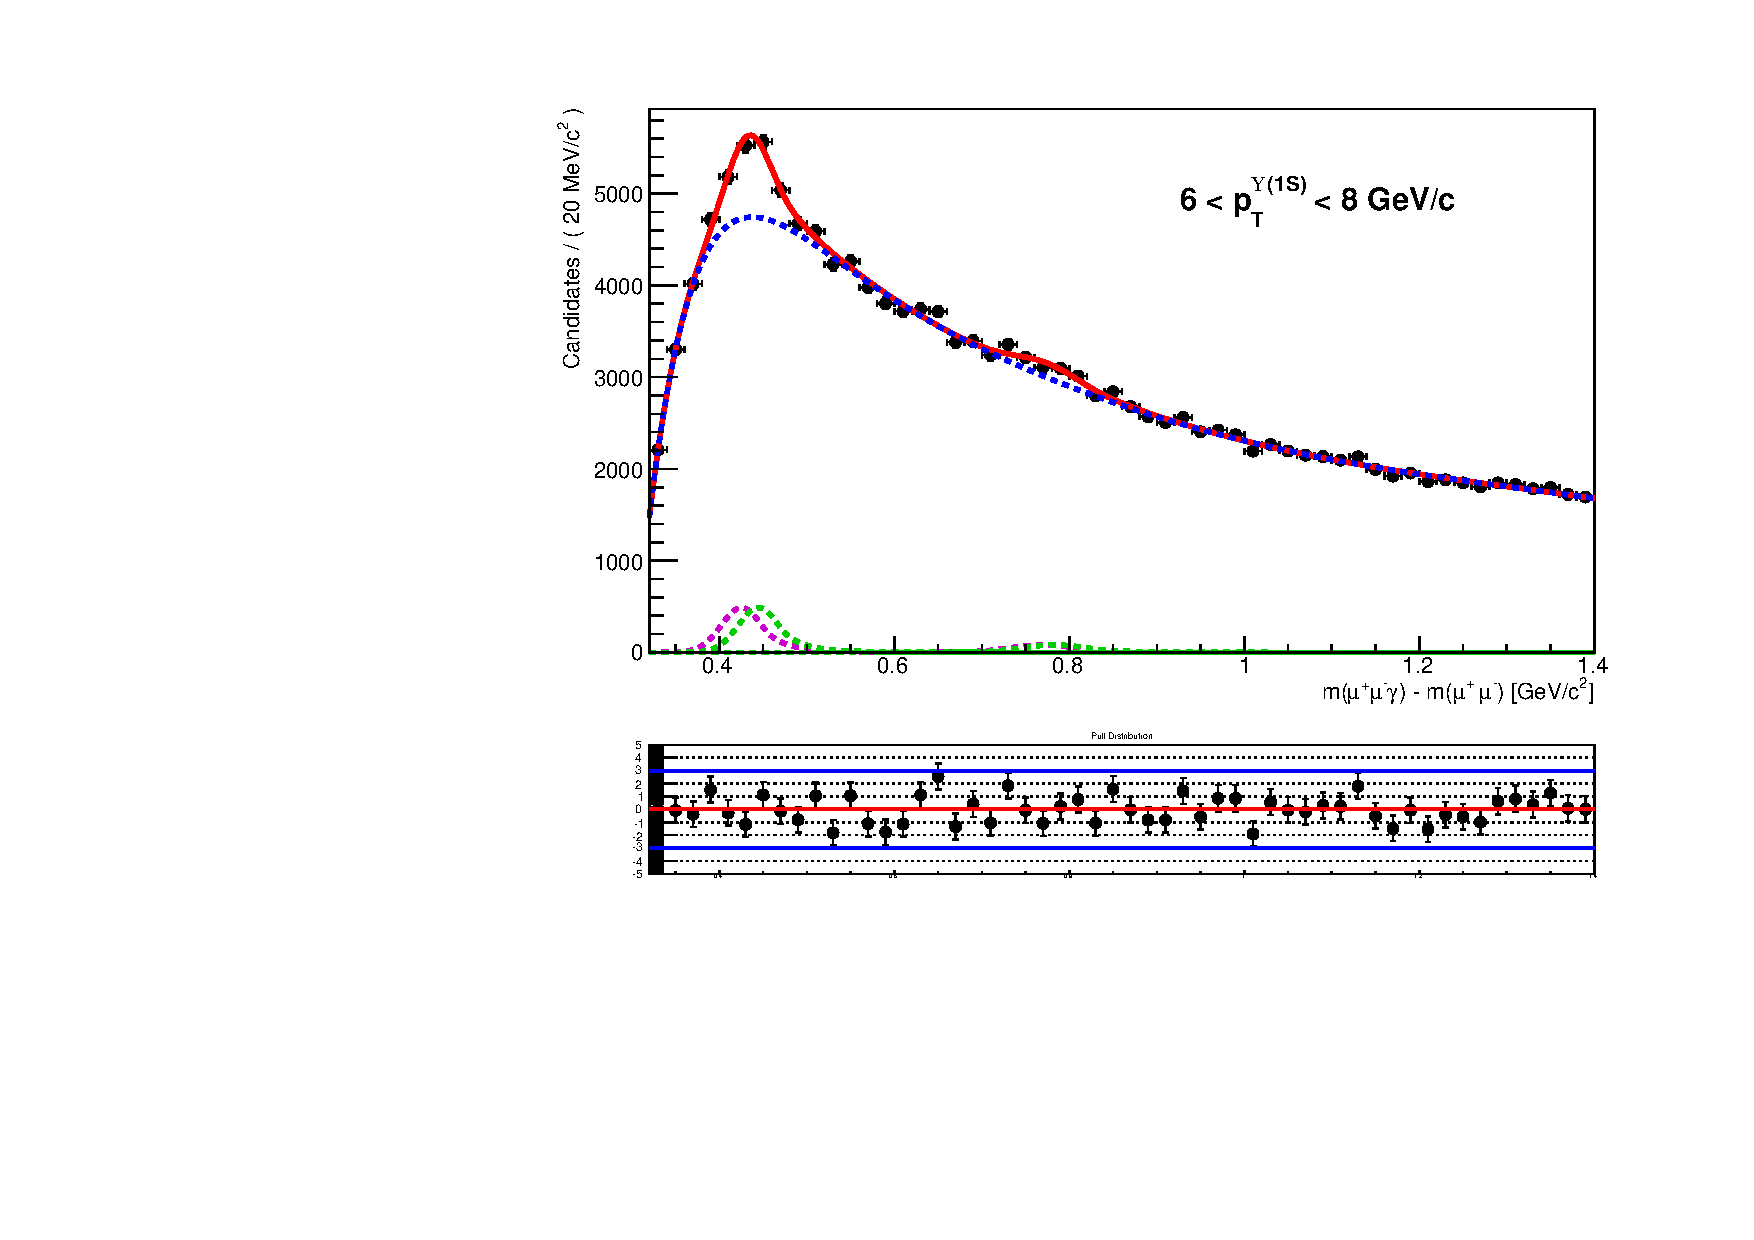
\includegraphics[width=0.31\linewidth]{chib_fits/fit_chib_2011_6_8}
      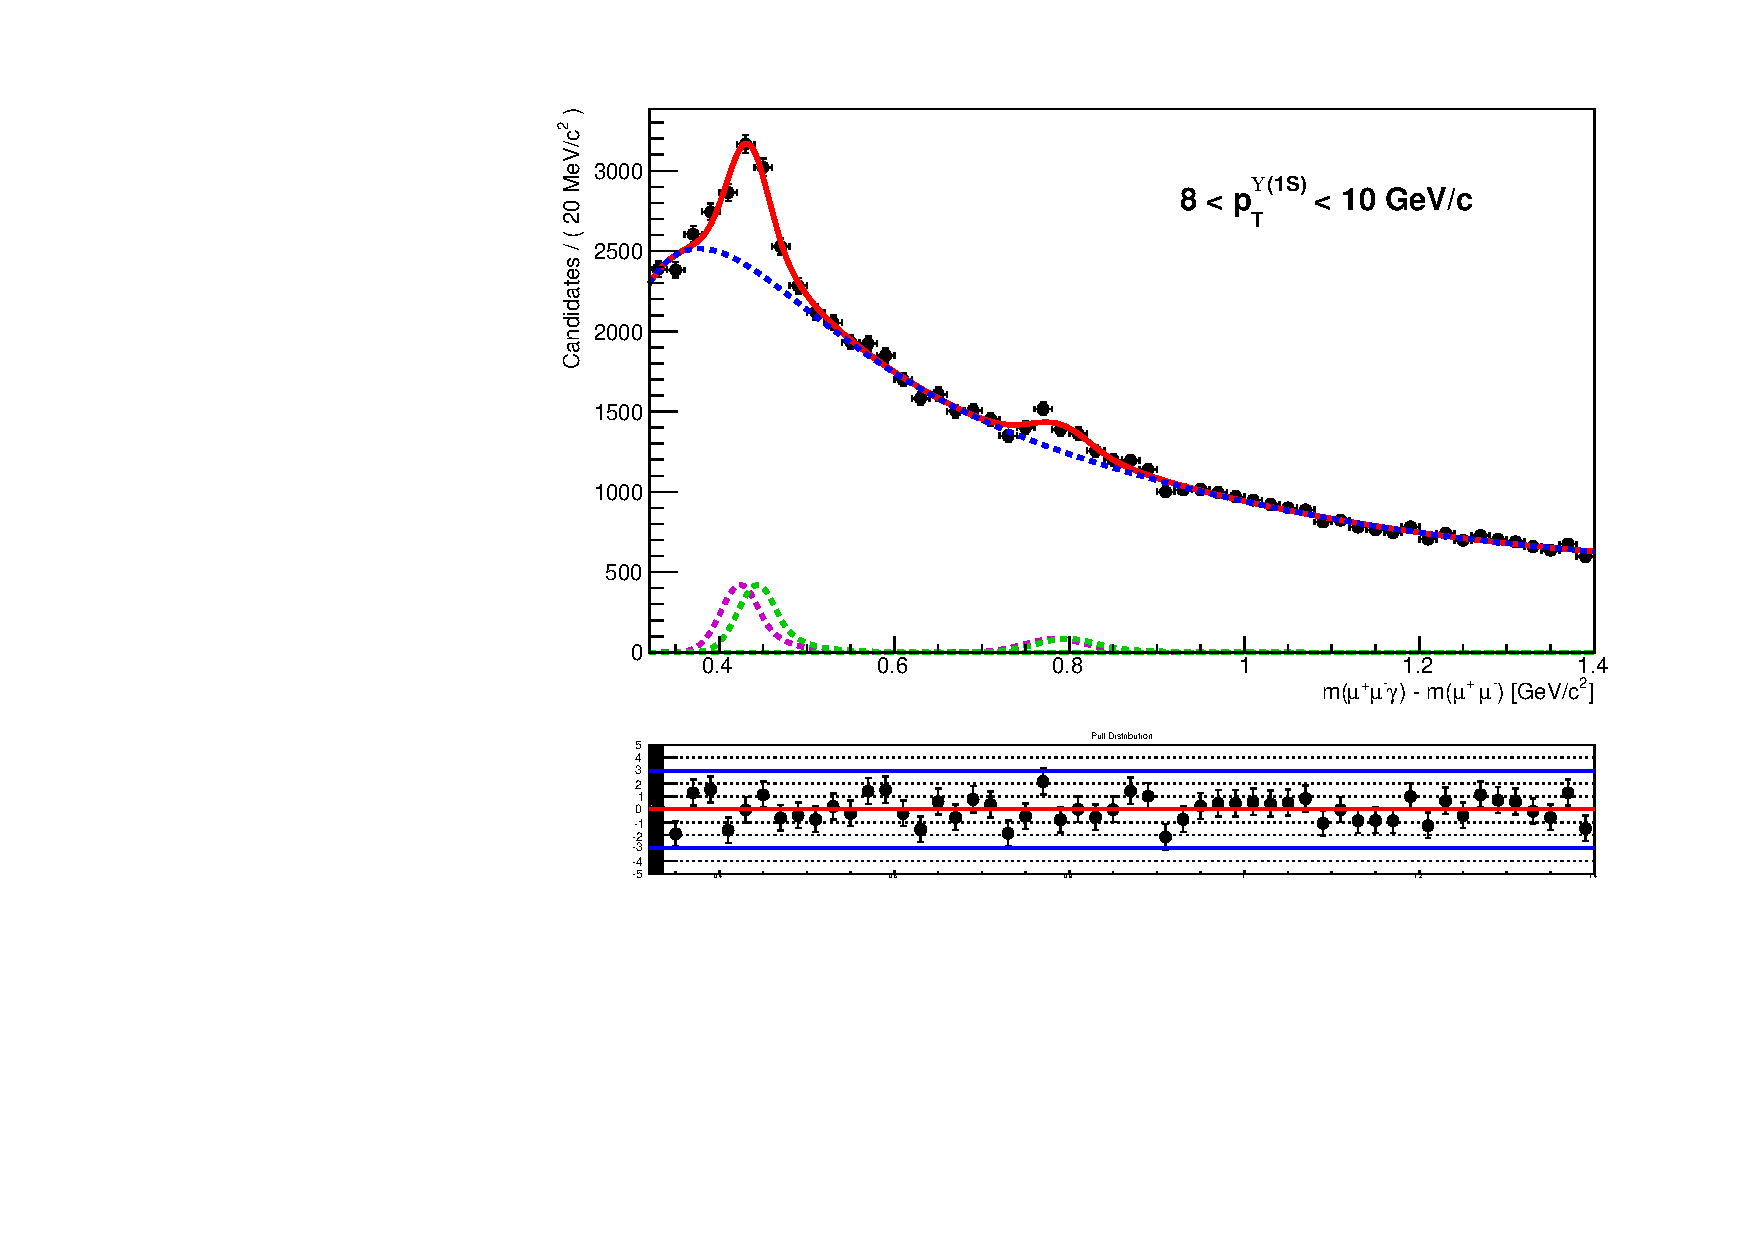
\includegraphics[width=0.31\linewidth]{chib_fits/fit_chib_2011_8_10}
      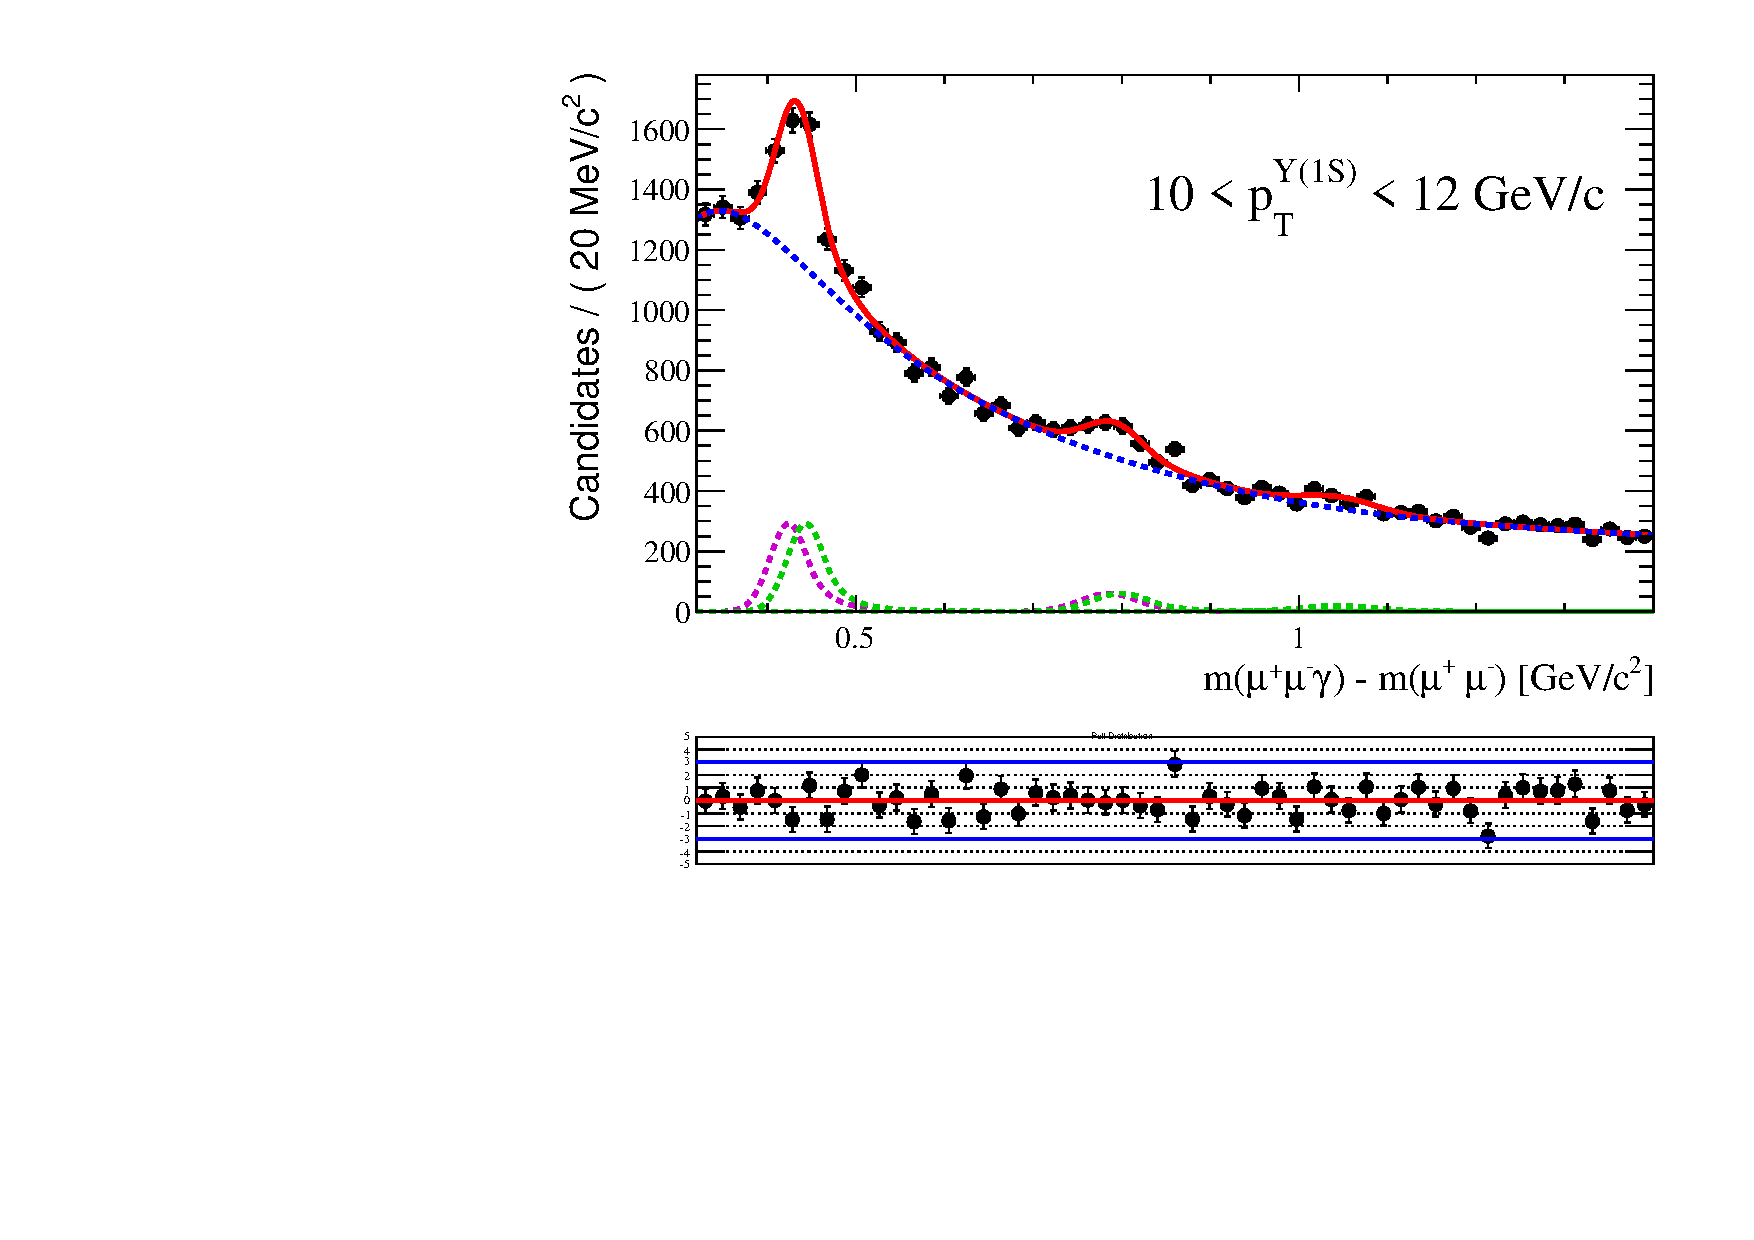
\includegraphics[width=0.31\linewidth]{chib_fits/fit_chib_2011_10_12}
      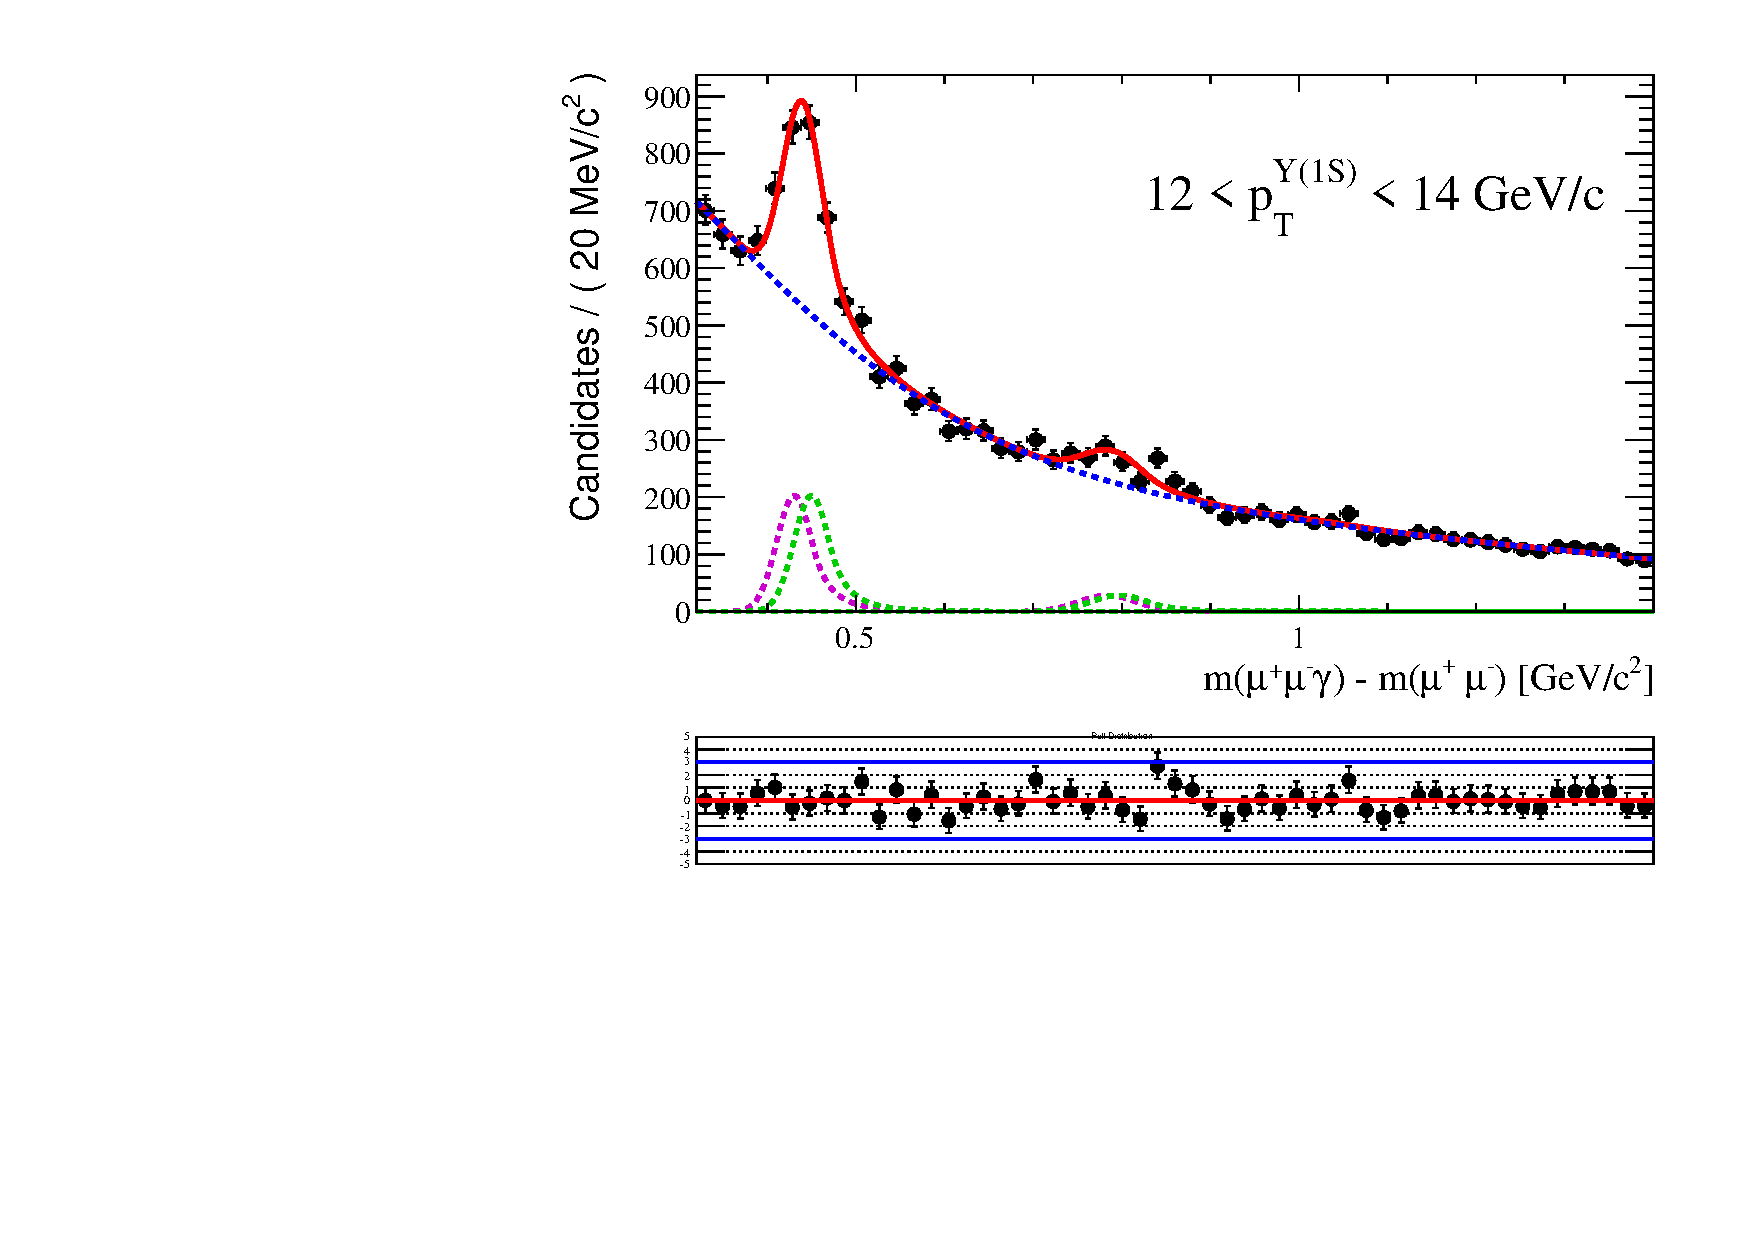
\includegraphics[width=0.31\linewidth]{chib_fits/fit_chib_2011_12_14}
      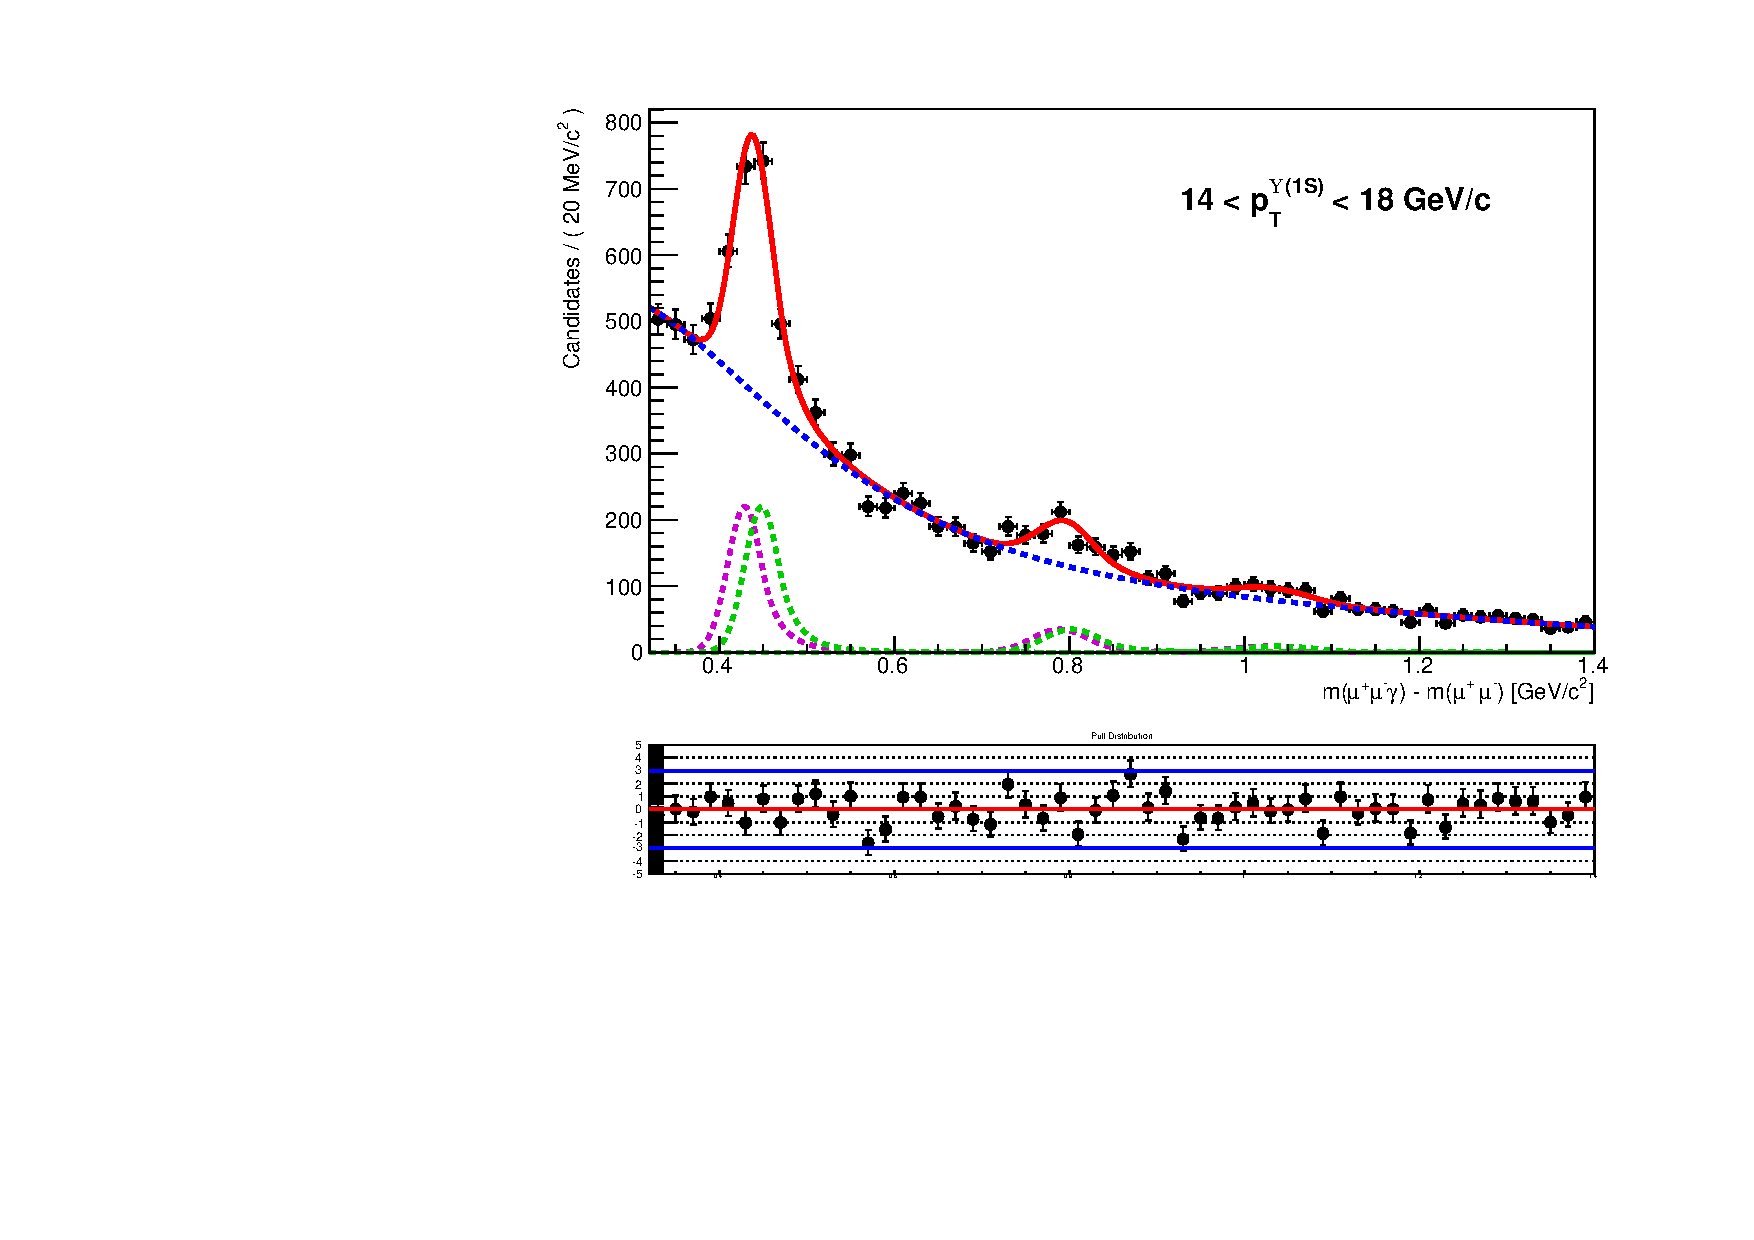
\includegraphics[width=0.31\linewidth]{chib_fits/fit_chib_2011_14_18}
      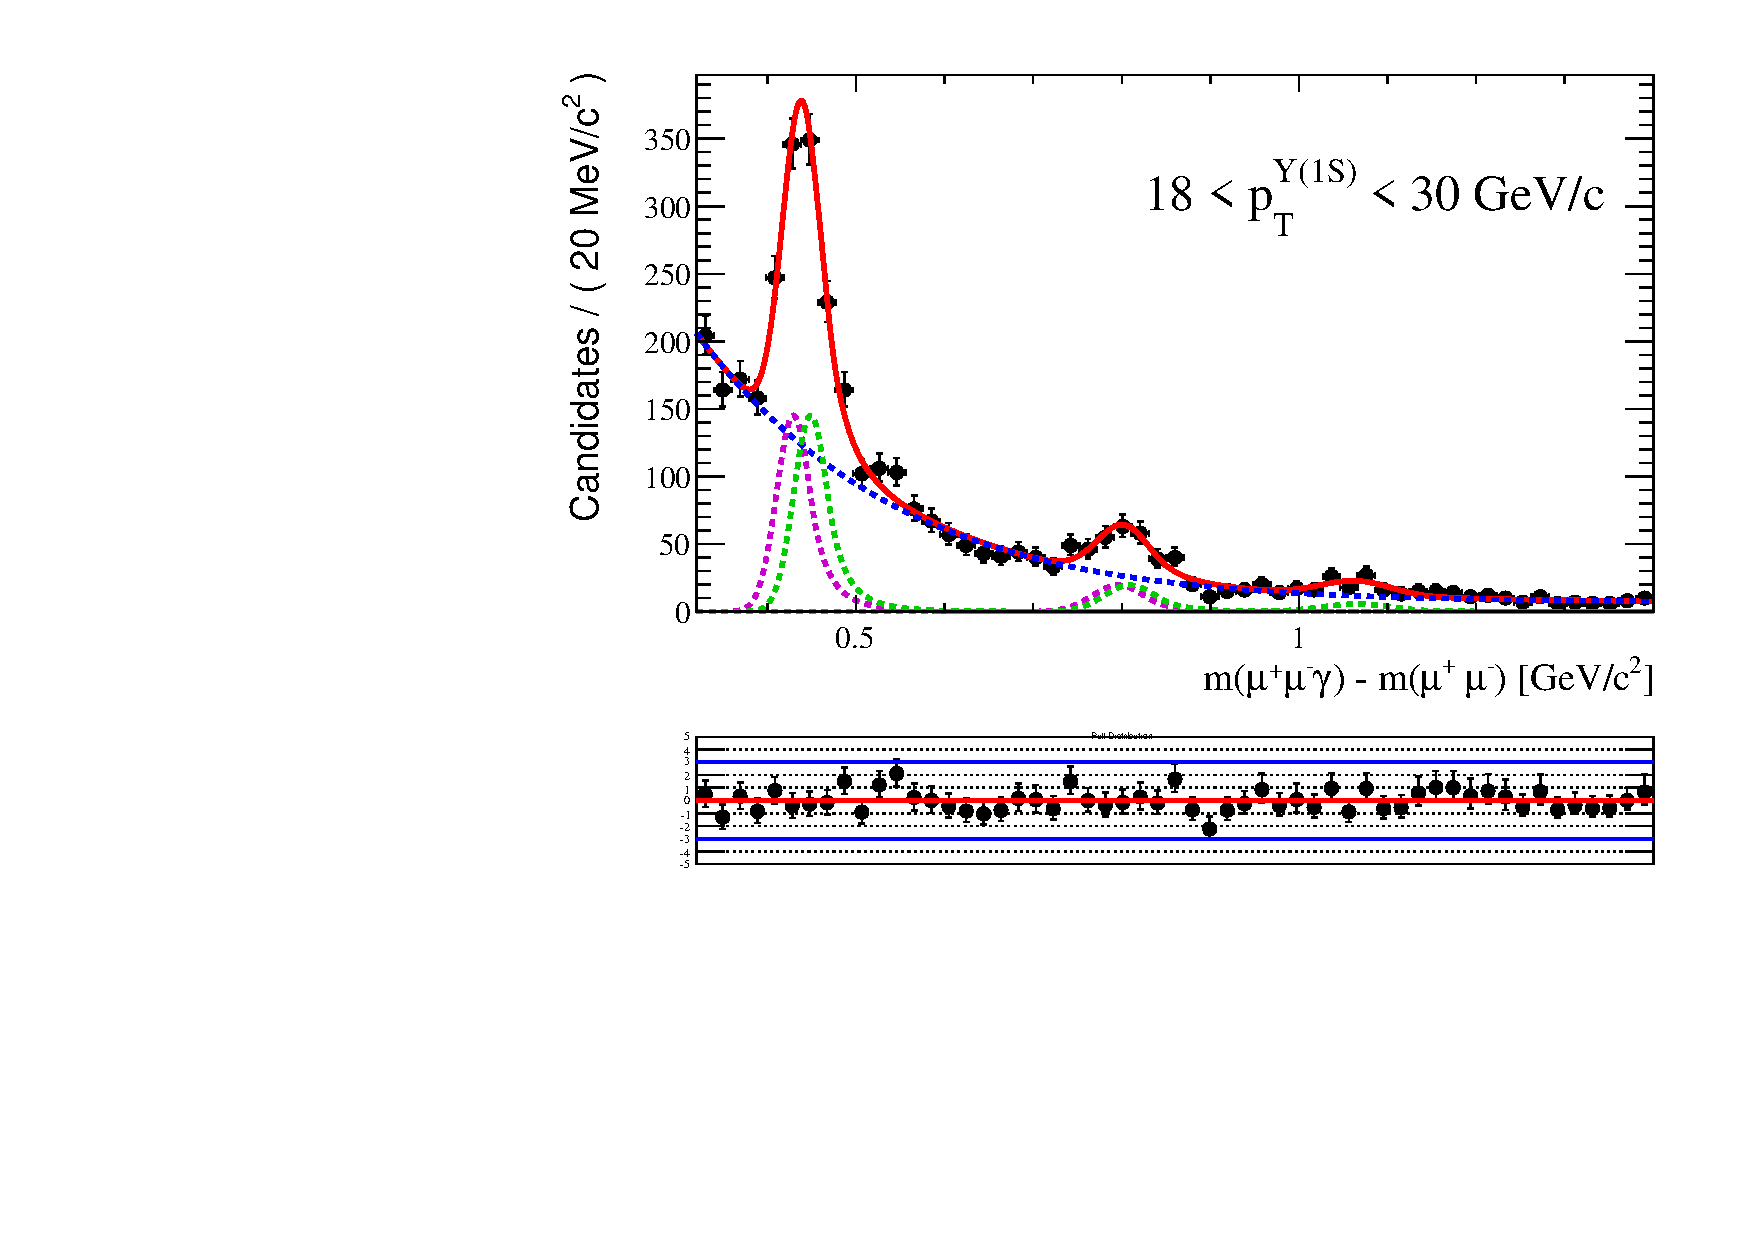
\includegraphics[width=0.31\linewidth]{chib_fits/fit_chib_2011_18_30}
      \caption{\sqs=7\tev (2011)}
      \label{fig:chib_fits_2011}
    \end{subfigure}
    \begin{subfigure}[b]{\textwidth}
      \centering
      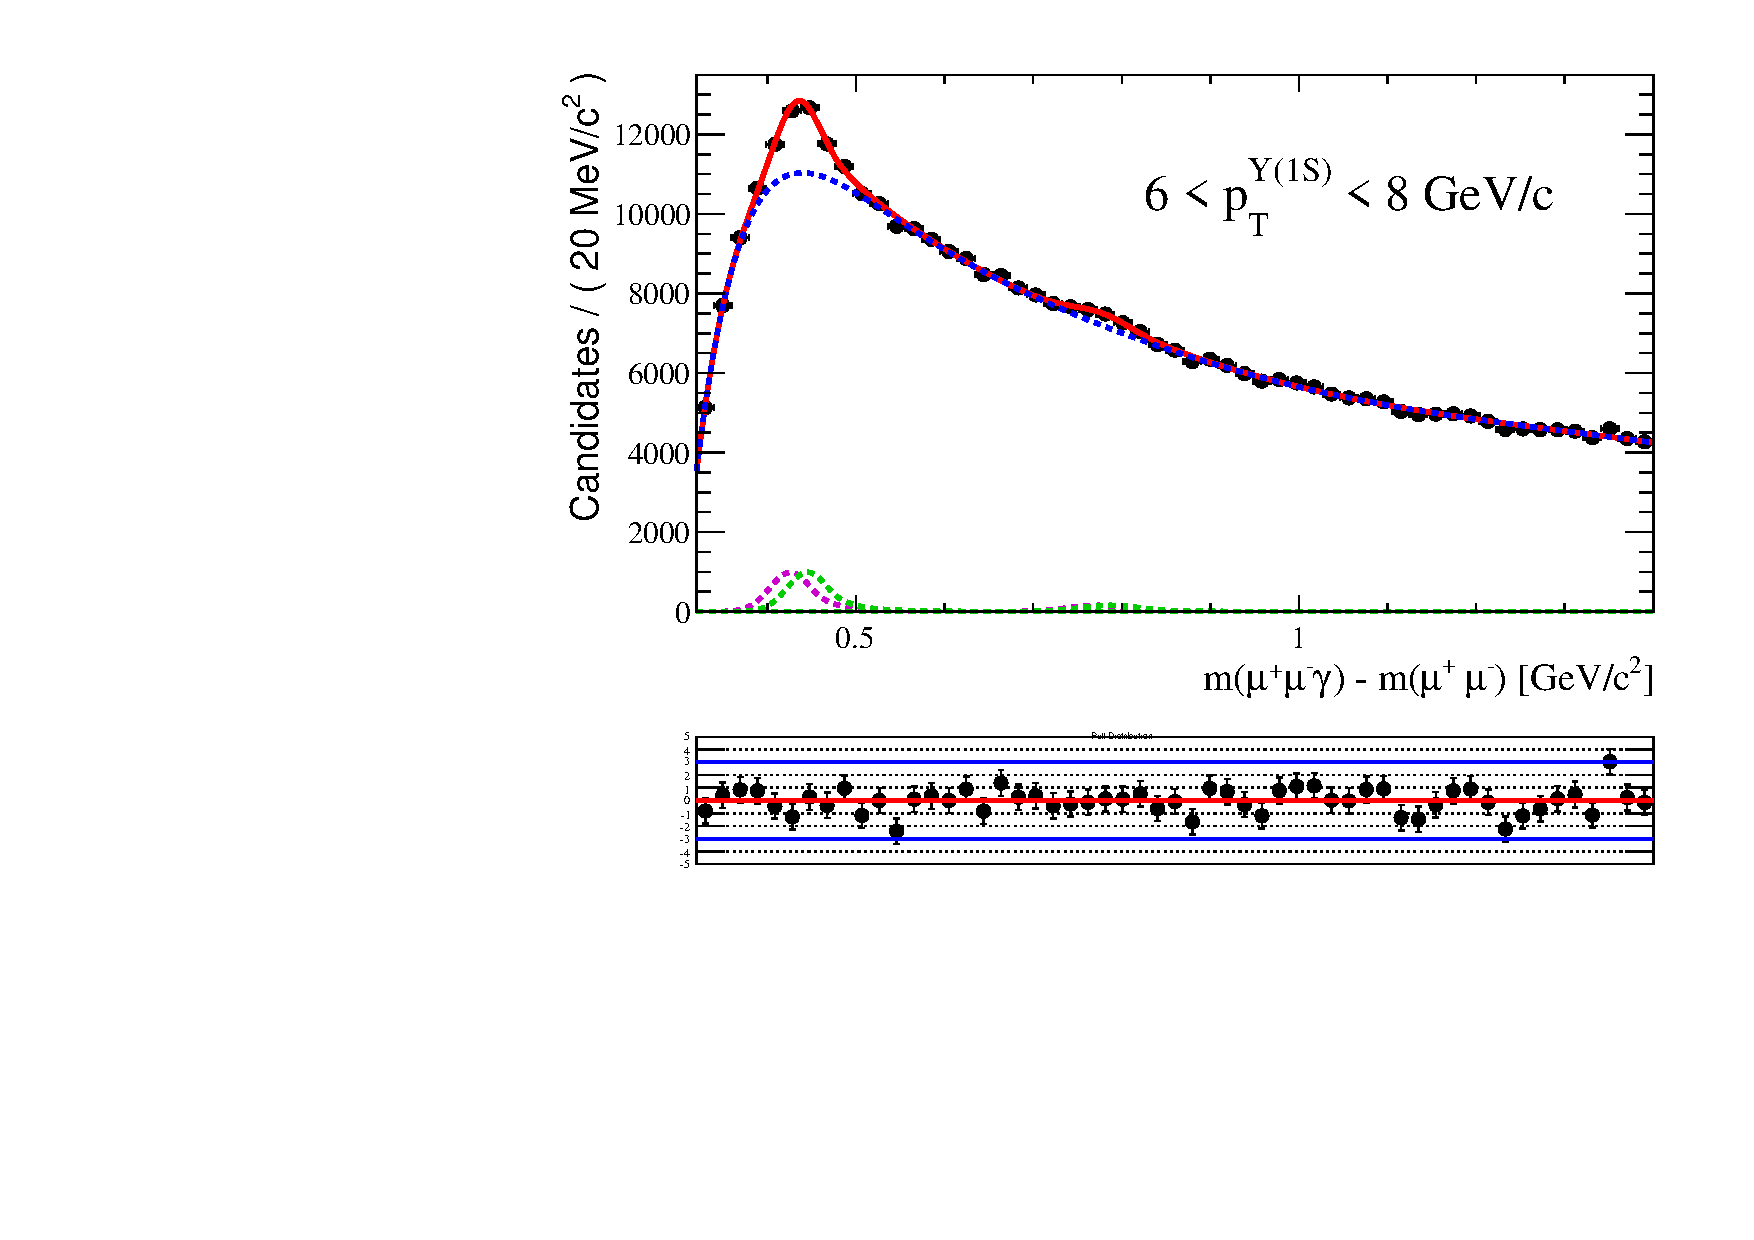
\includegraphics[width=0.31\linewidth]{chib_fits/fit_chib_2012_6_8}
      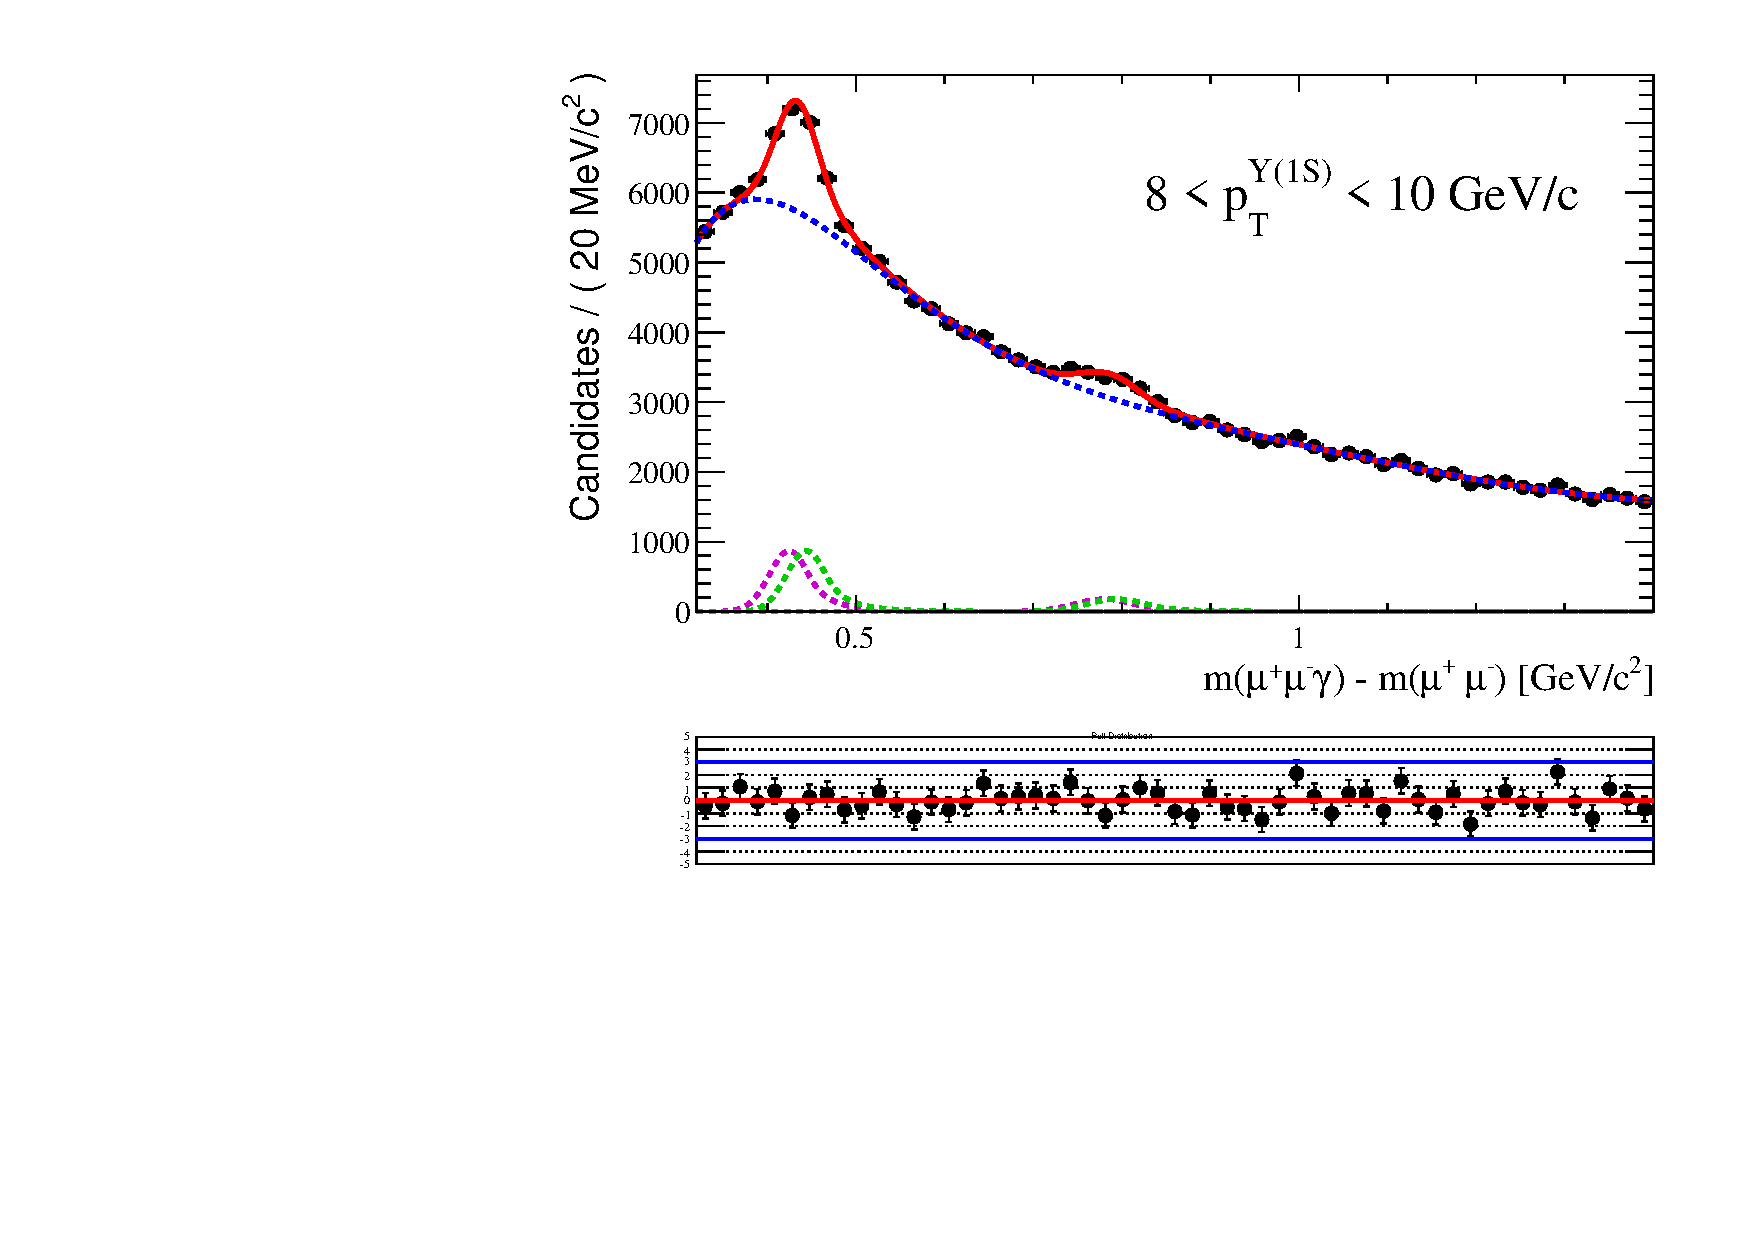
\includegraphics[width=0.31\linewidth]{chib_fits/fit_chib_2012_8_10}
      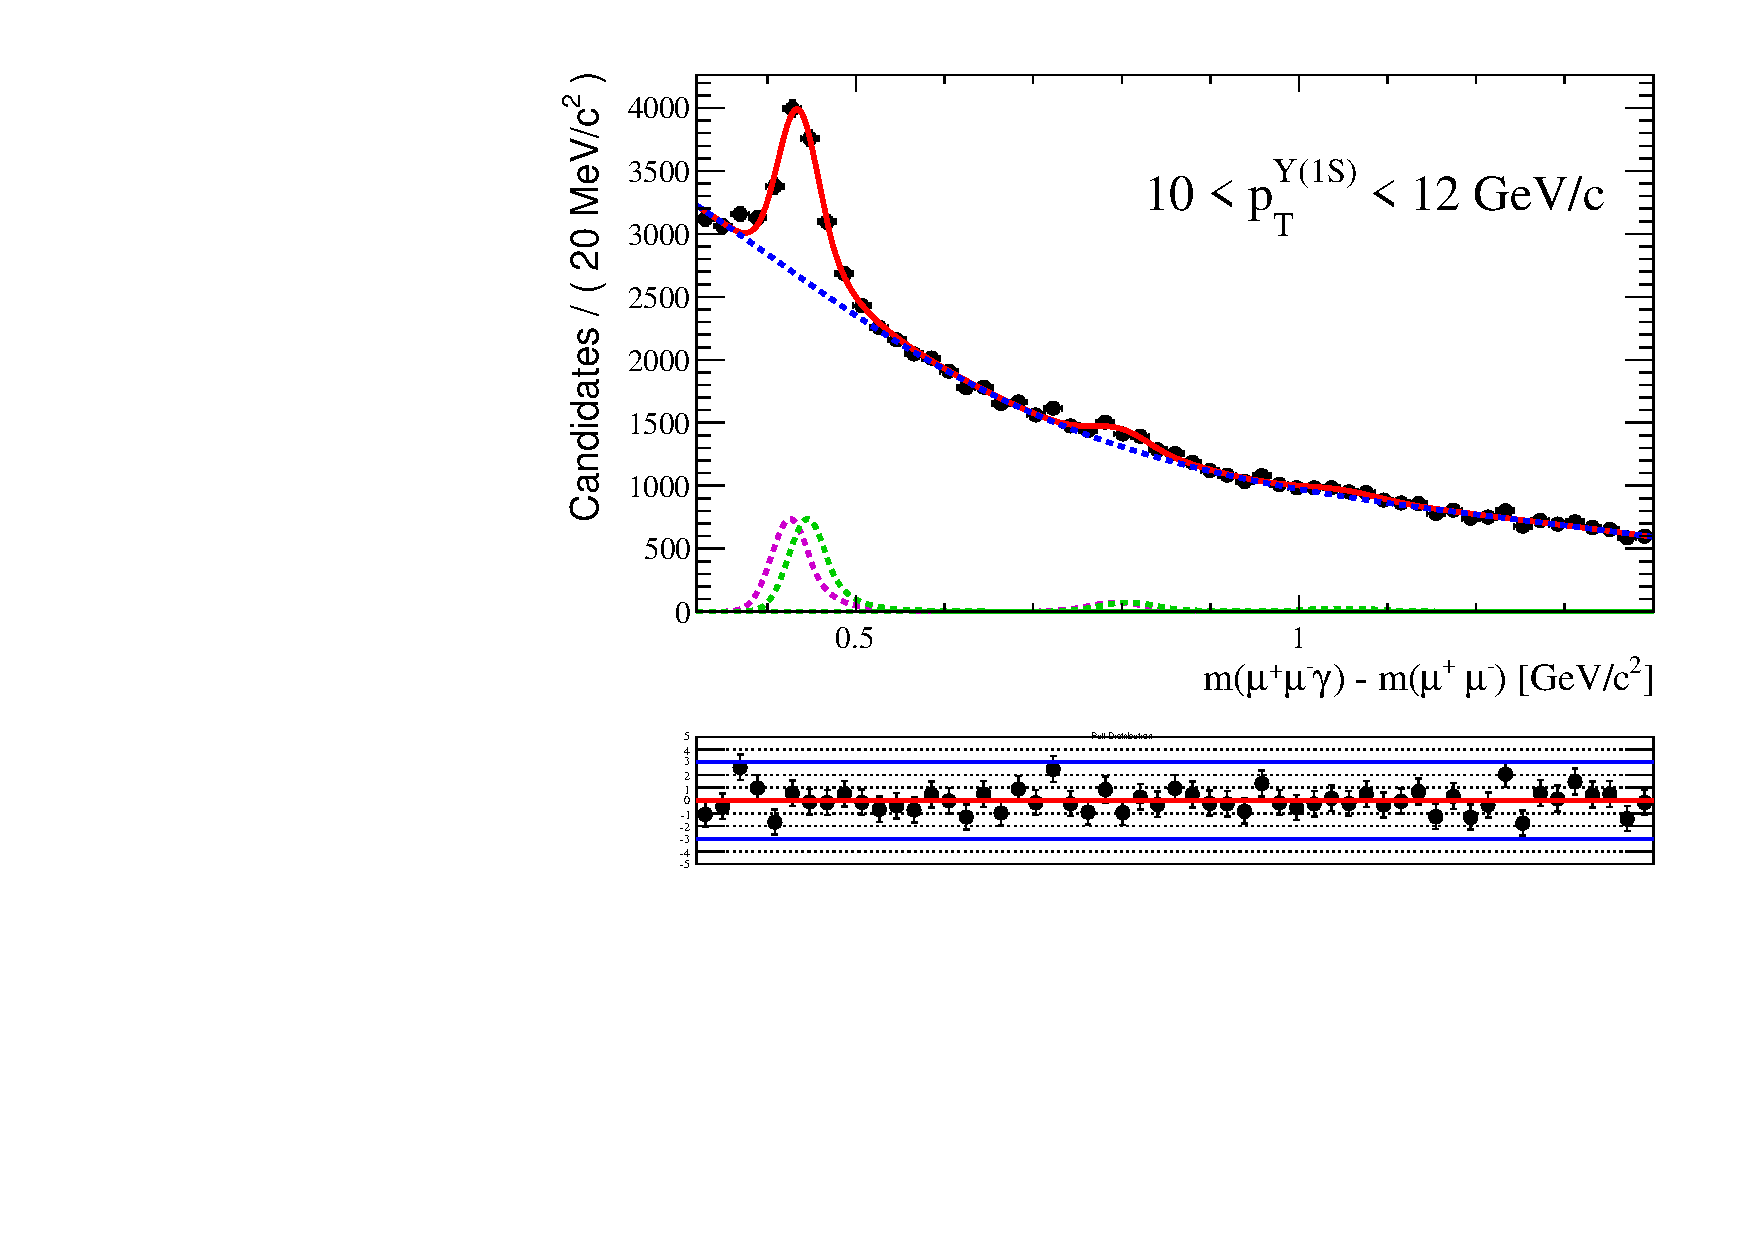
\includegraphics[width=0.31\linewidth]{chib_fits/fit_chib_2012_10_12}
      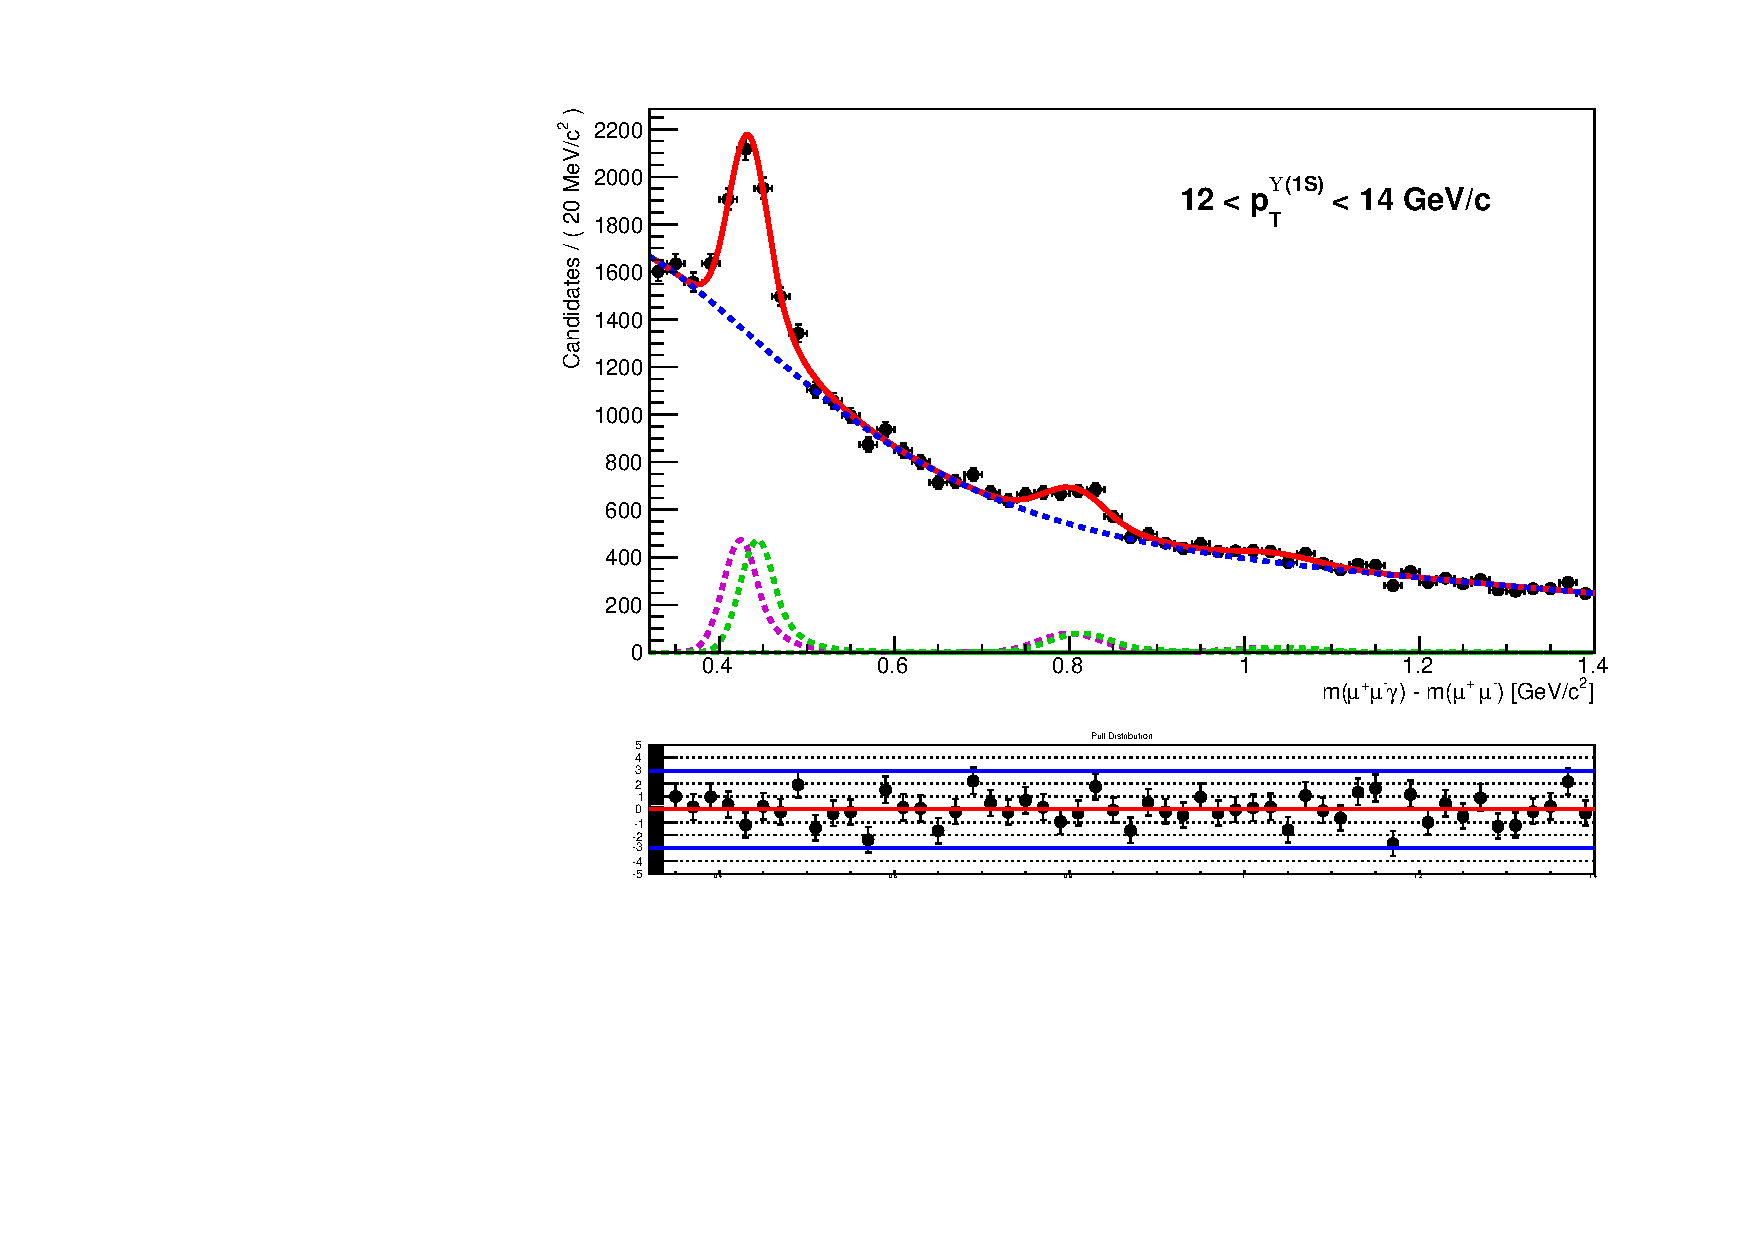
\includegraphics[width=0.31\linewidth]{chib_fits/fit_chib_2012_12_14}
      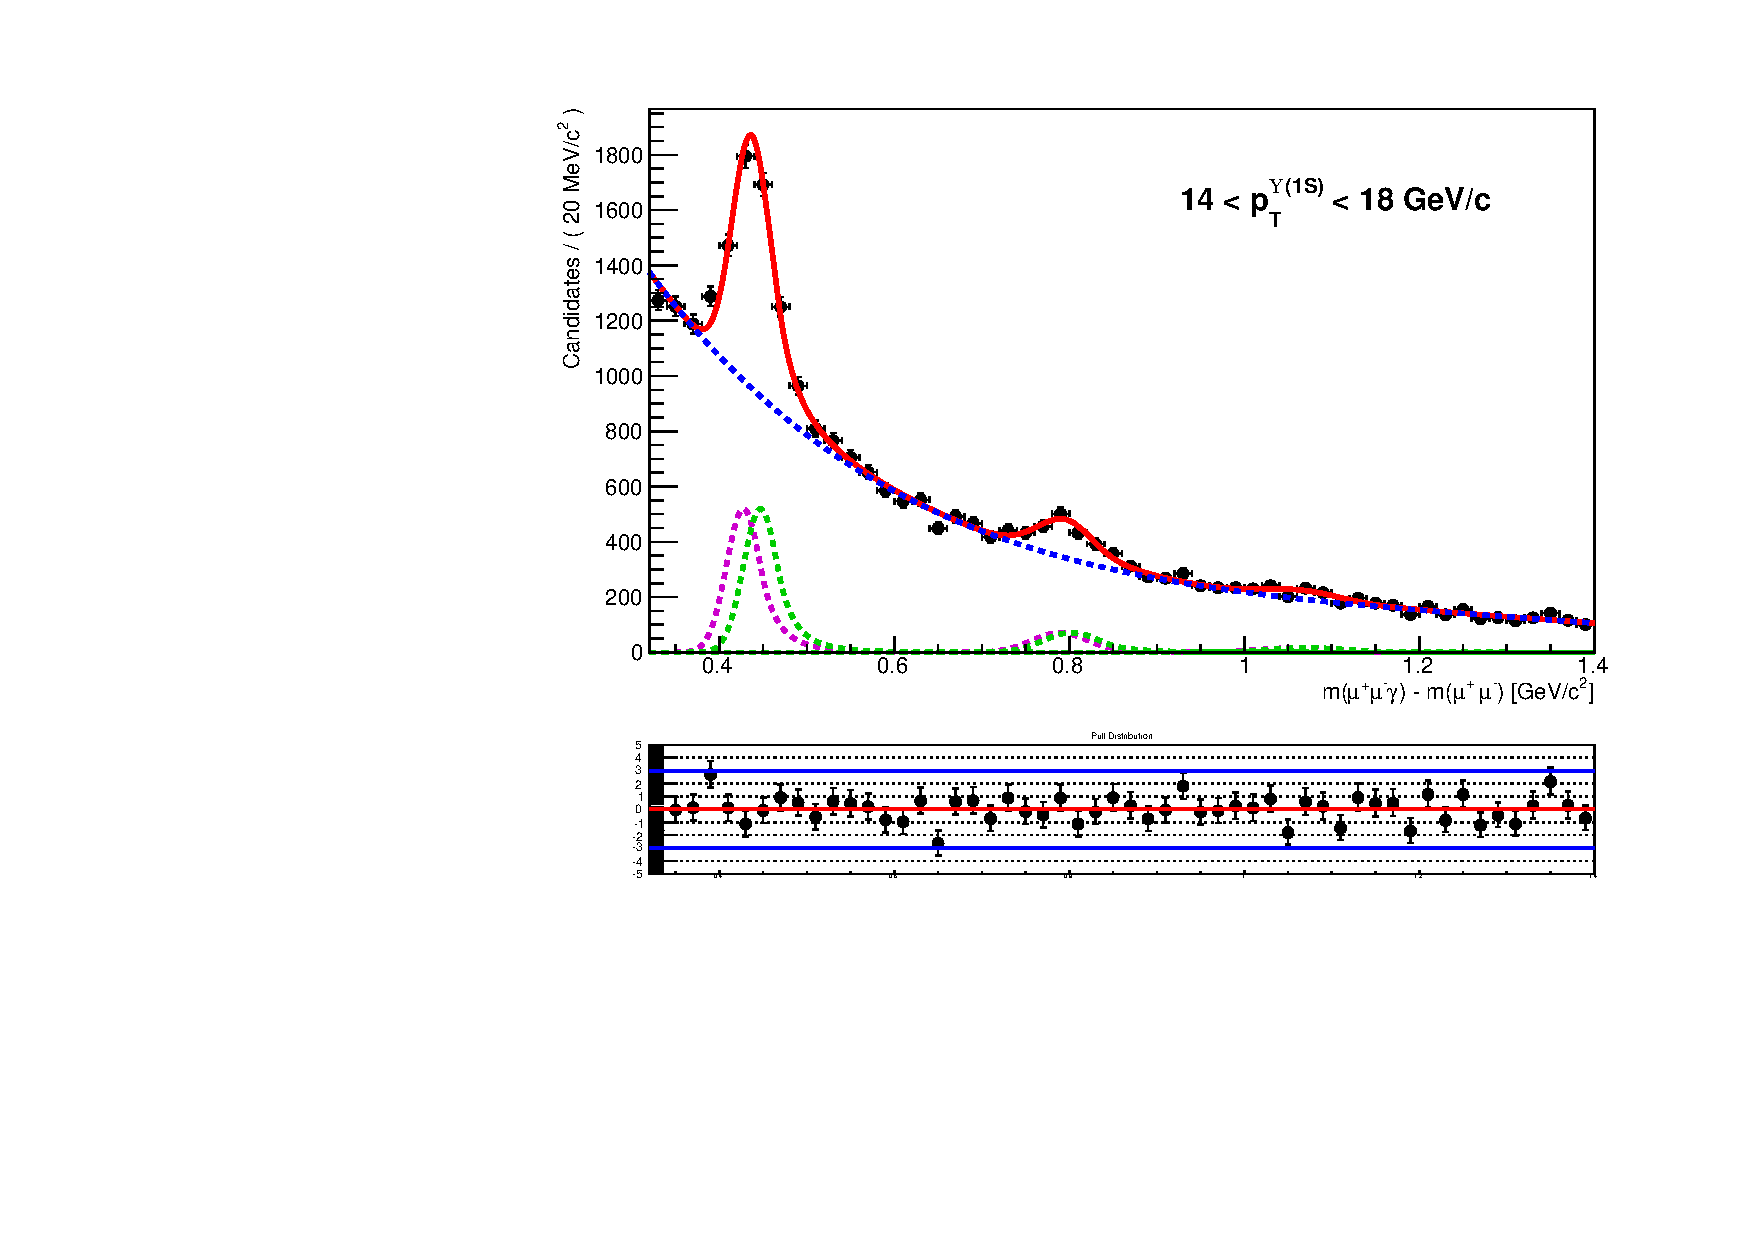
\includegraphics[width=0.31\linewidth]{chib_fits/fit_chib_2012_14_18}
      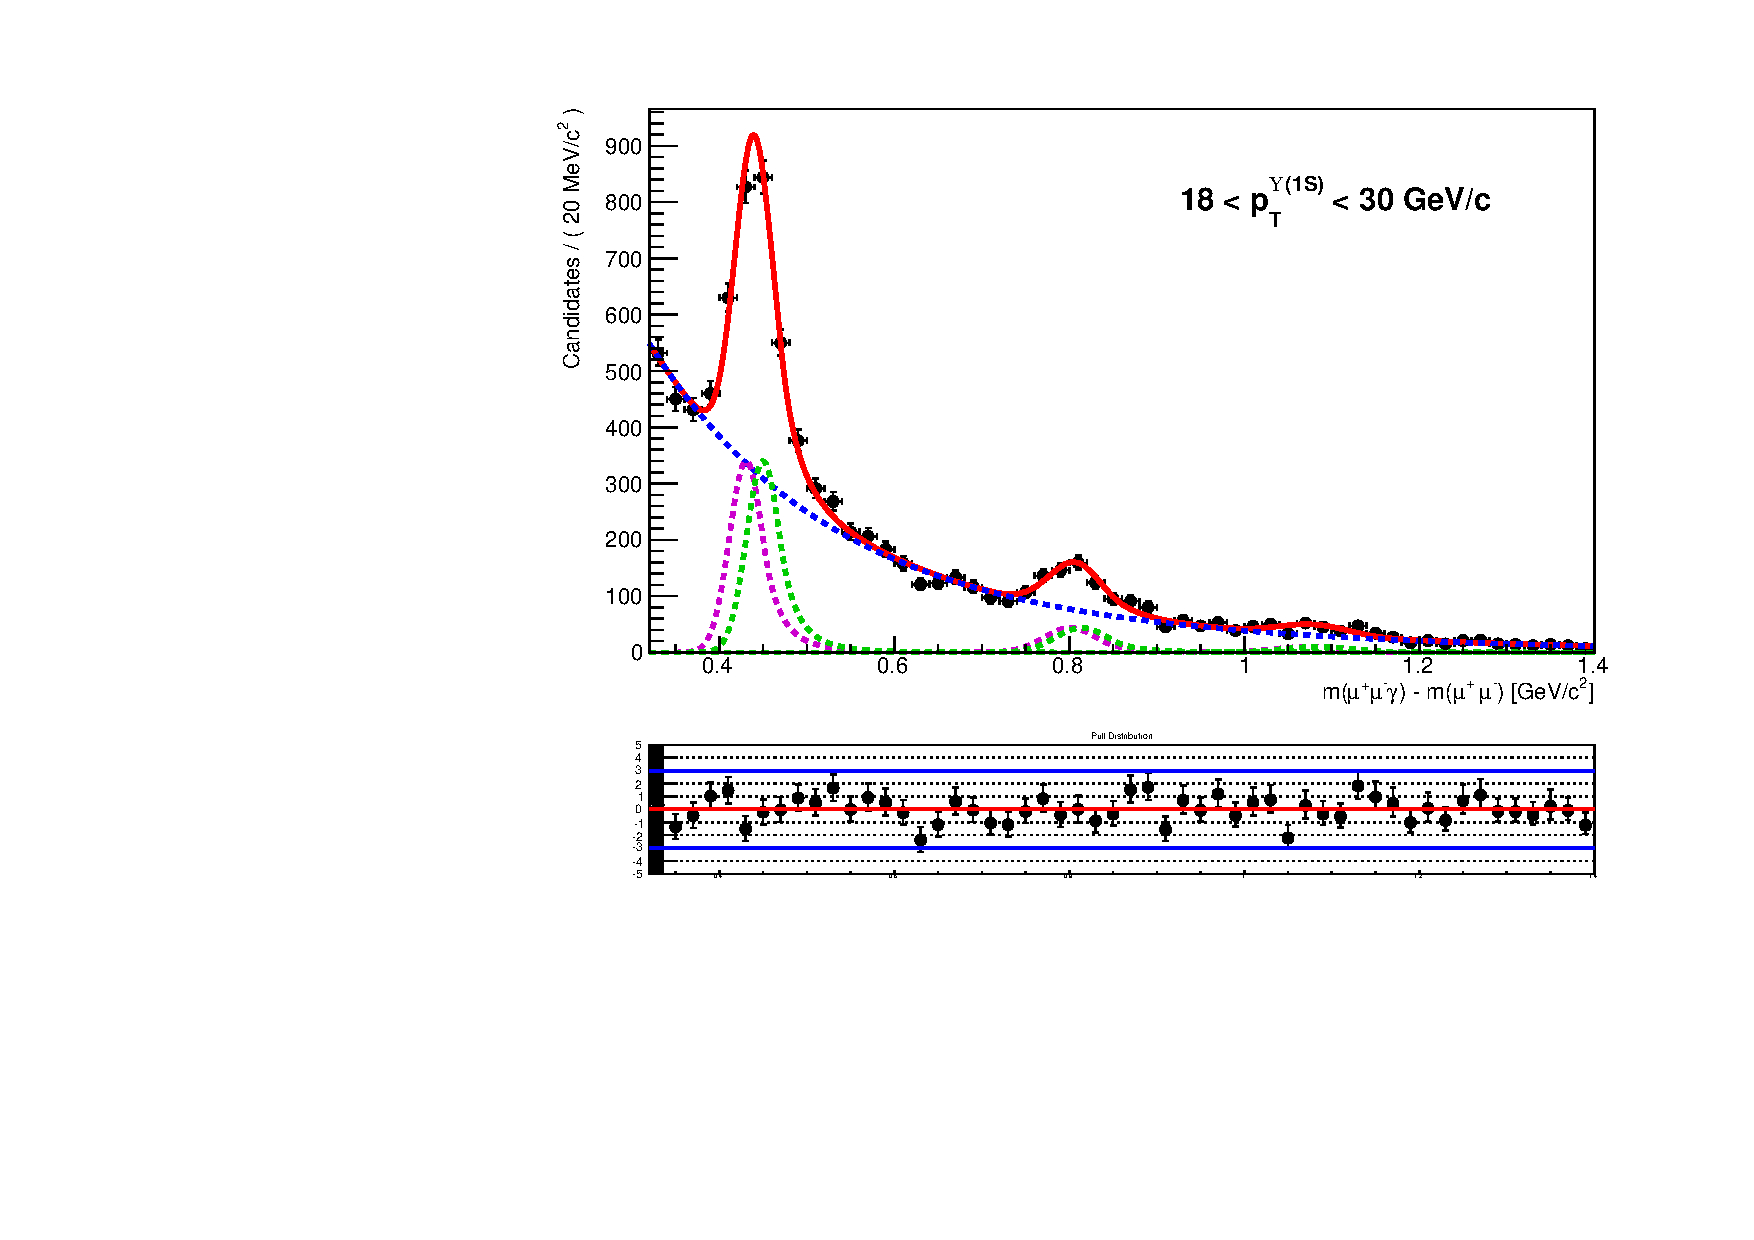
\includegraphics[width=0.31\linewidth]{chib_fits/fit_chib_2012_18_30}
      \caption{\sqs=8\tev (2012)}
      \label{fig:chib_fits_2012}
    \end{subfigure}
  \caption{
    \small  Mass difference of the $\mumu \gamma$ system and $\mumu$ system for the 
    data for specified interval of transverse momentum of the \OneS. The red
    solid line is the result of the fit described in the text. Blue dashed line 
    is the background contribution obtained from the fit. Magenta and green 
    dashed lines are \chibone and \chibtwo signal contribution obtained from the fit.
  }
  \label{fig:chib_fits}
\end{figure}


\begin{figure}[ht]
  \centering
    \begin{subfigure}[b]{\textwidth}
      \centering
      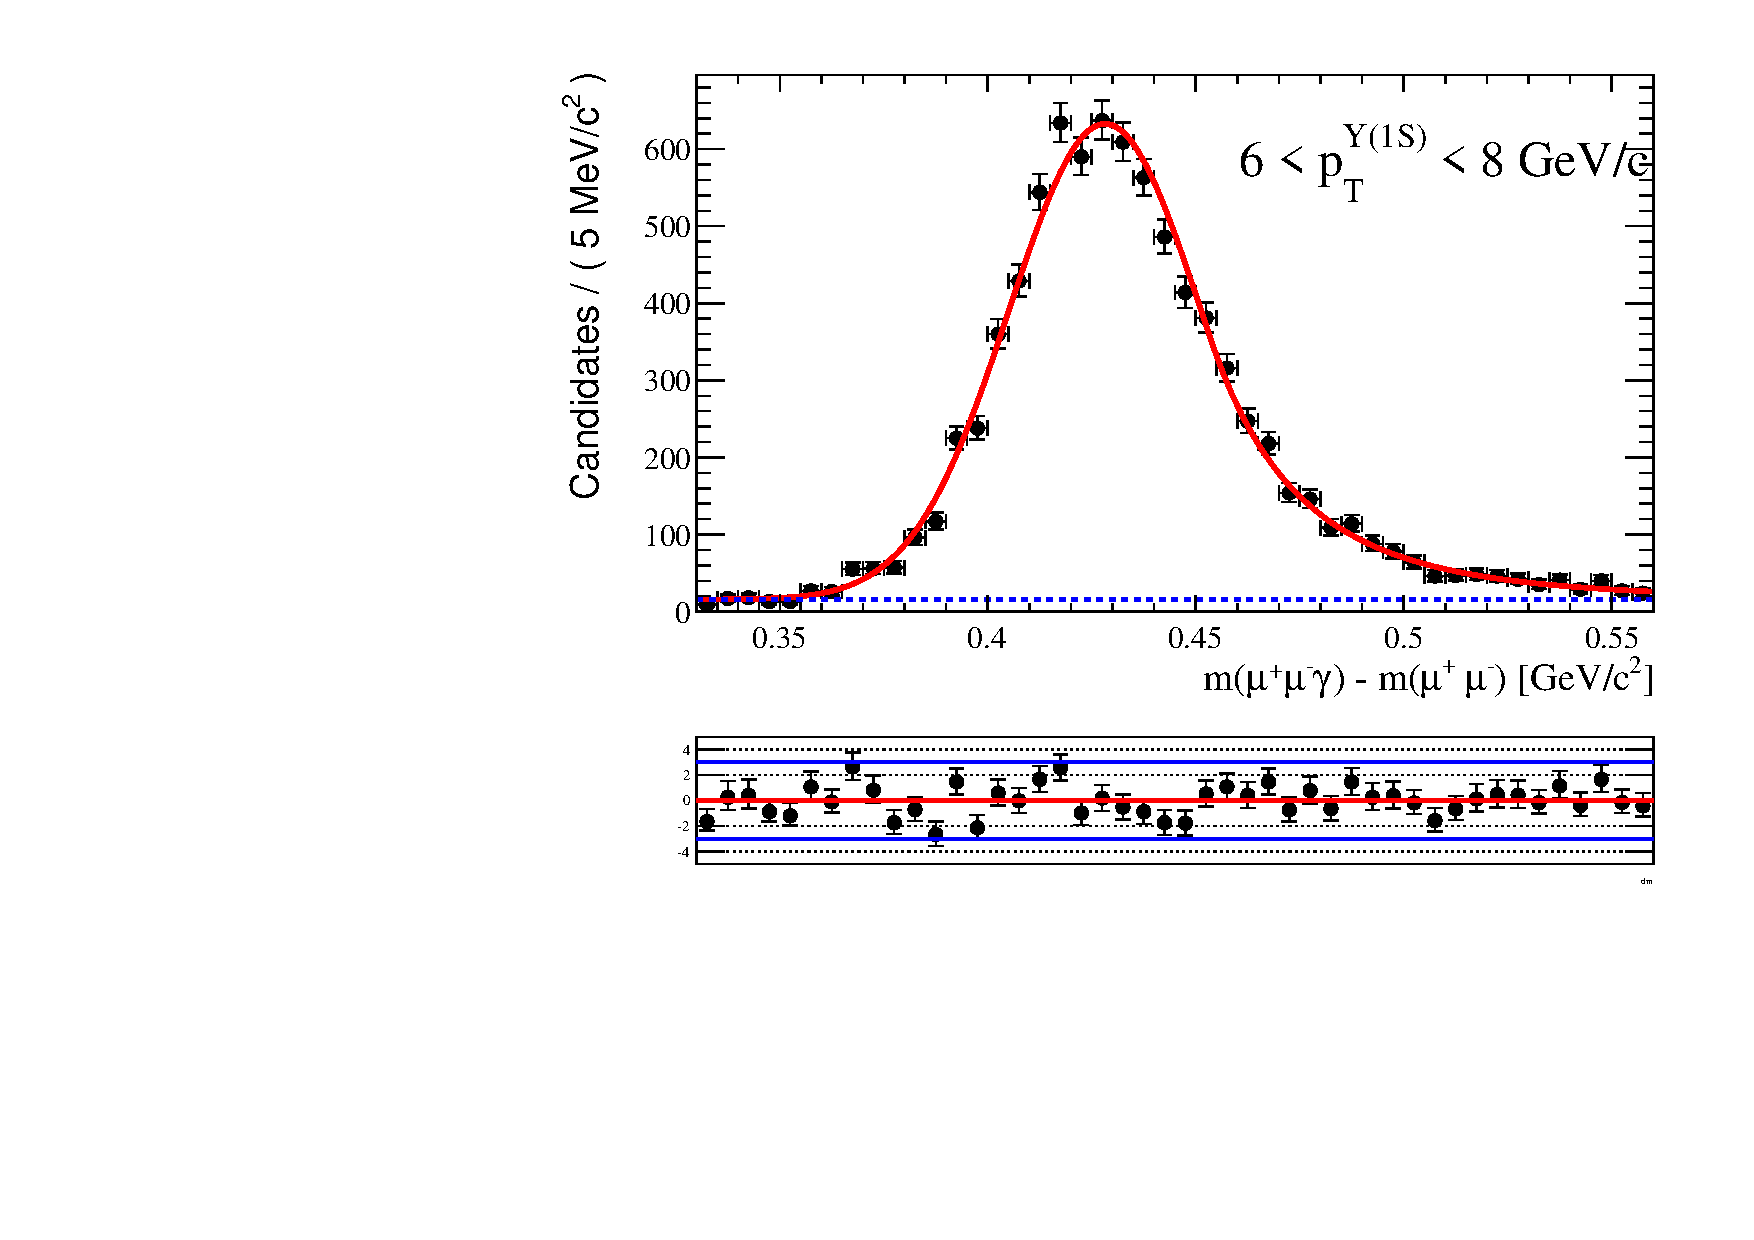
\includegraphics[width=0.16\linewidth]{fit_mc/chib11_6_8}
      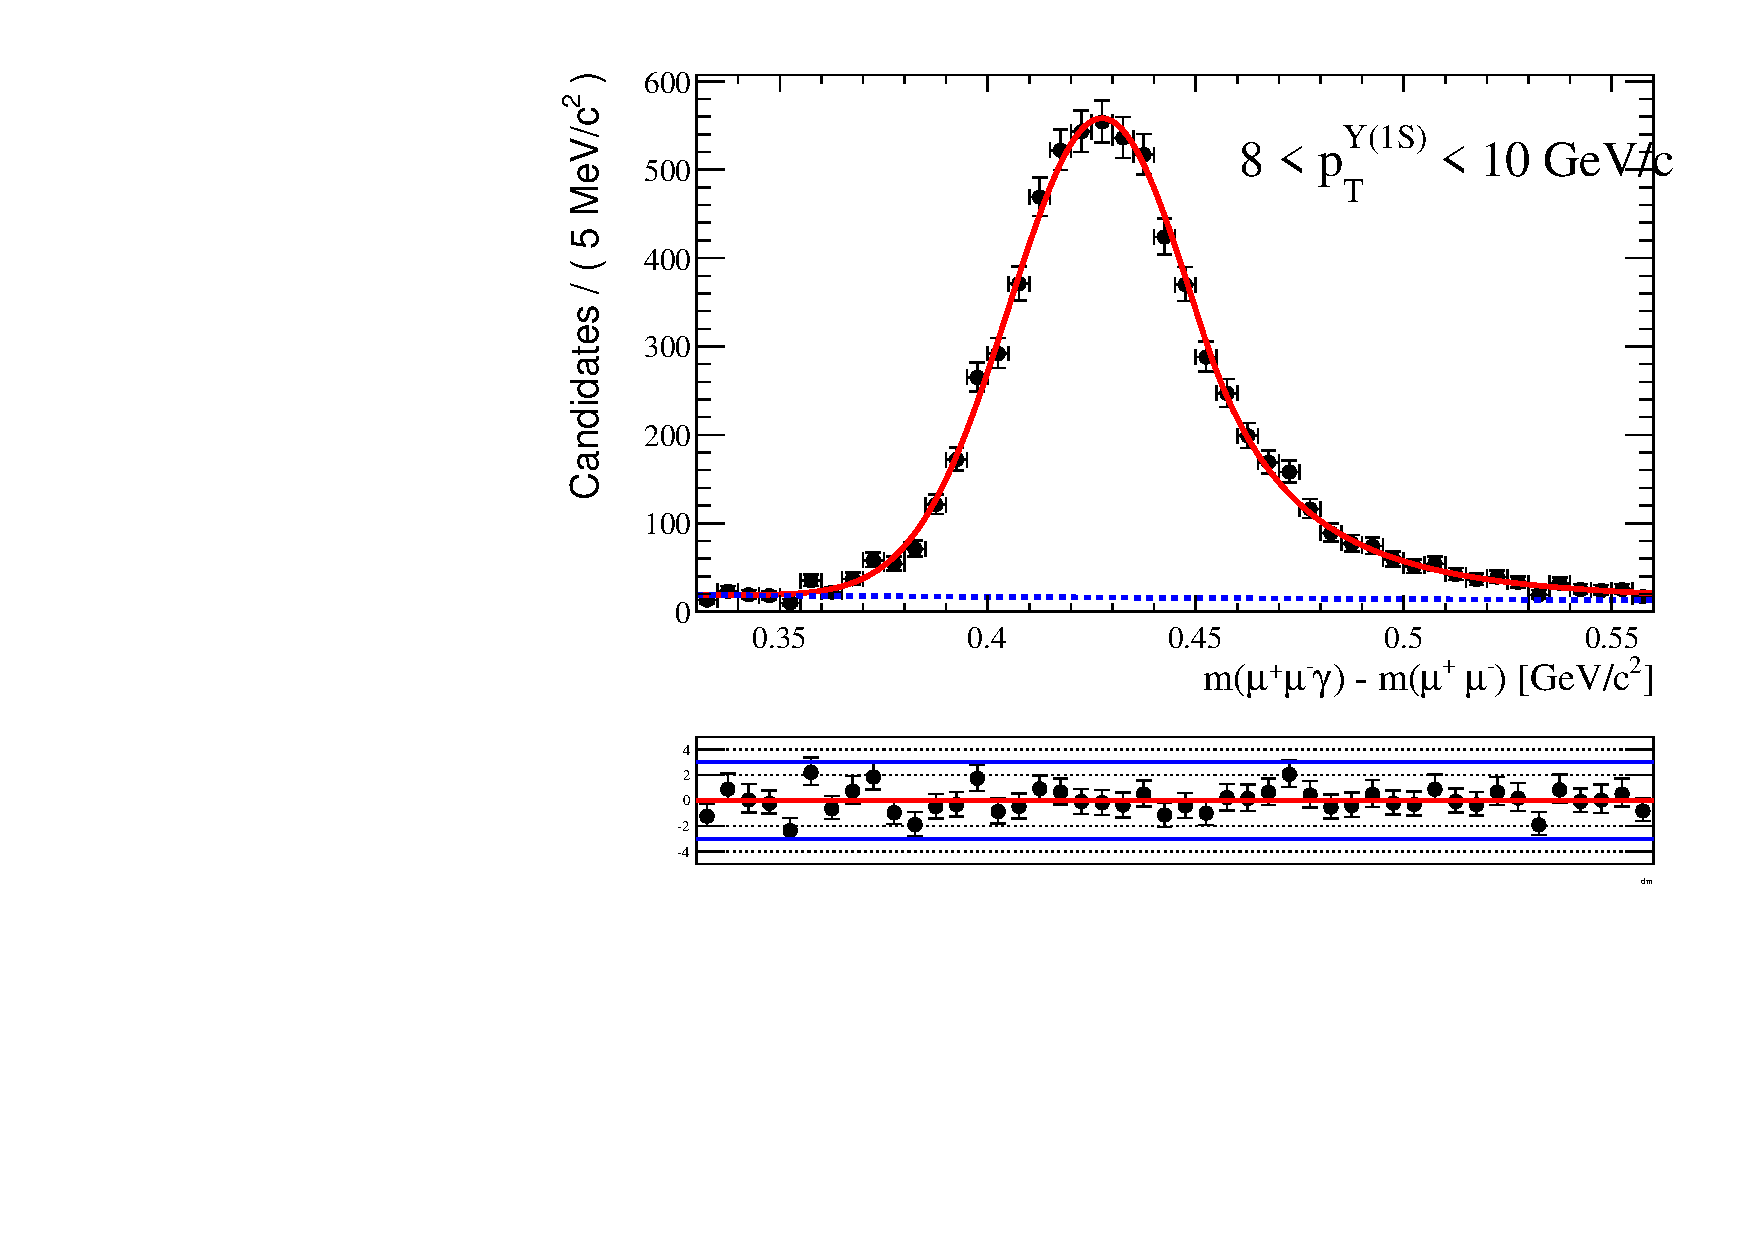
\includegraphics[width=0.16\linewidth]{fit_mc/chib11_8_10}
      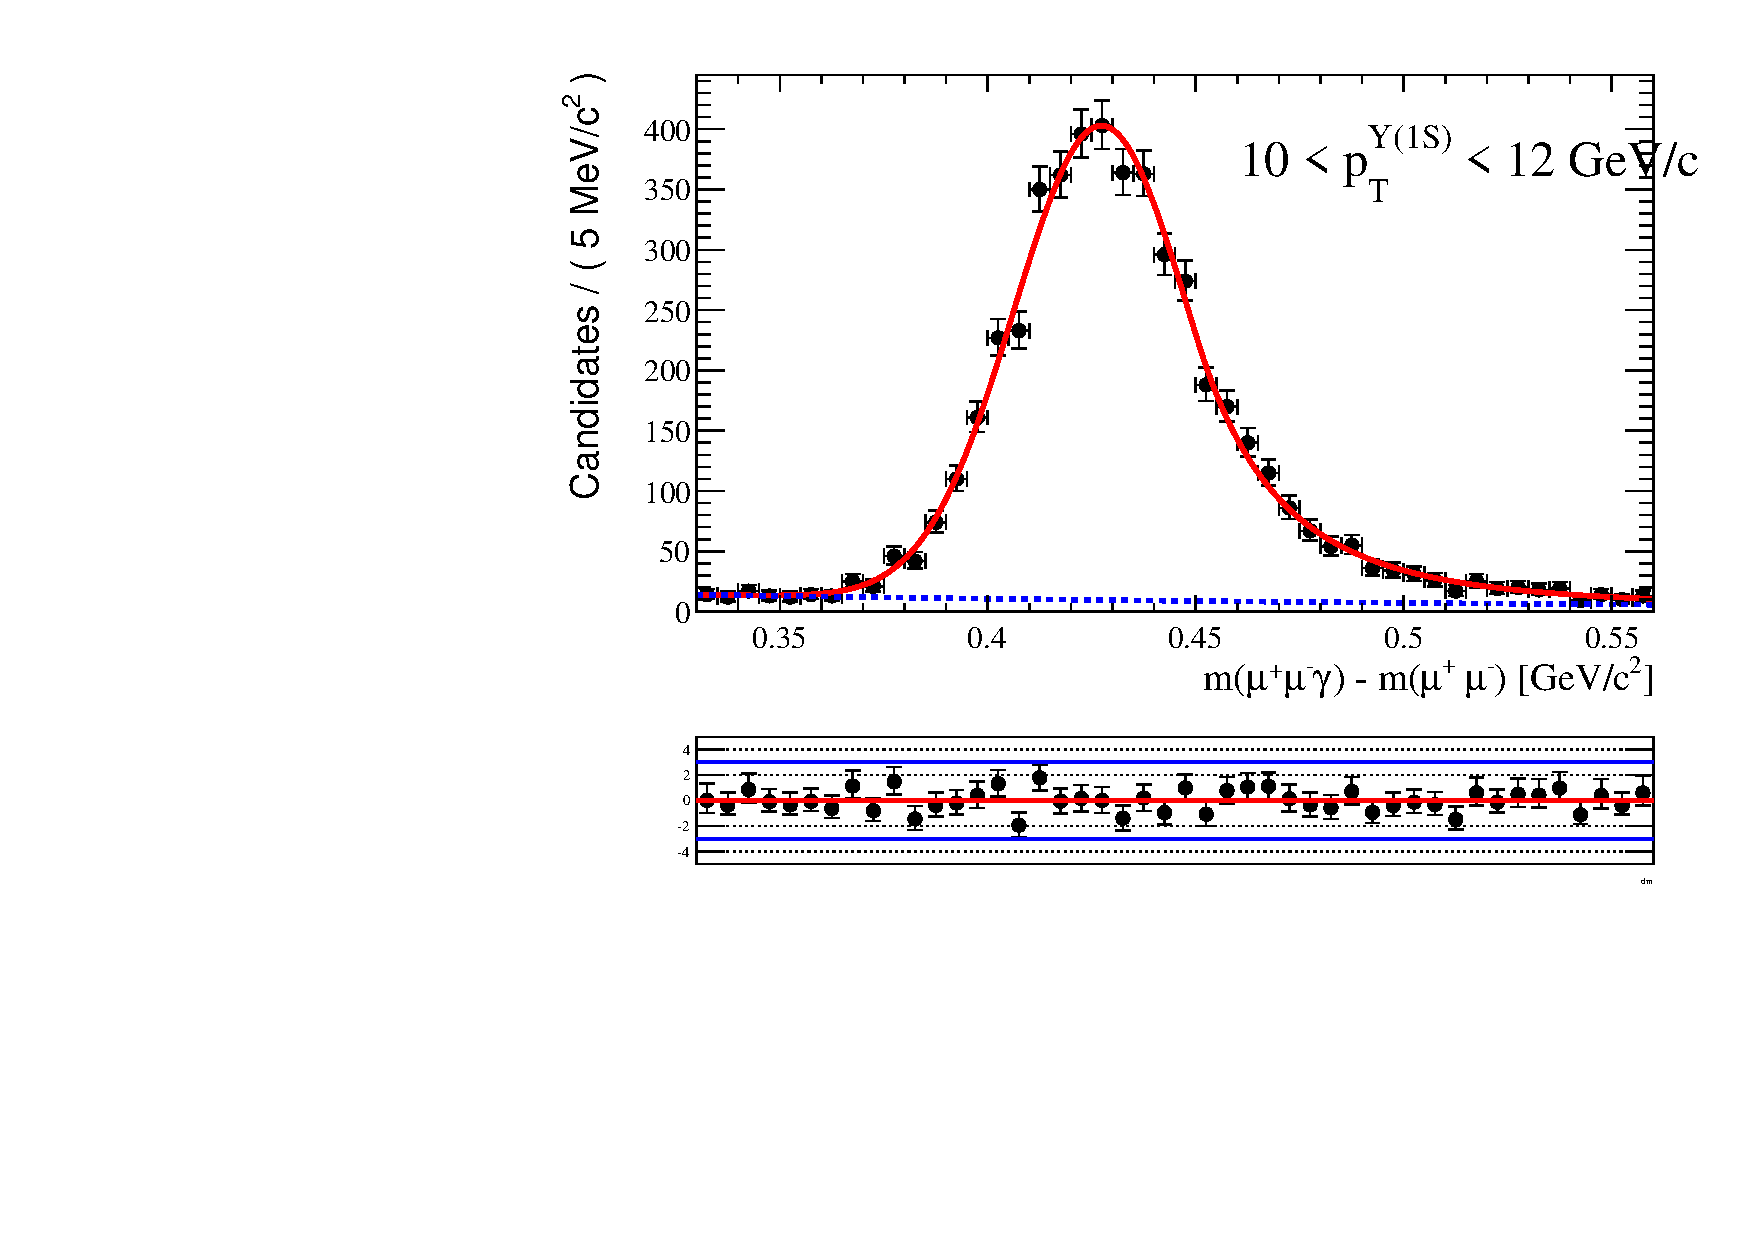
\includegraphics[width=0.16\linewidth]{fit_mc/chib11_10_12}
      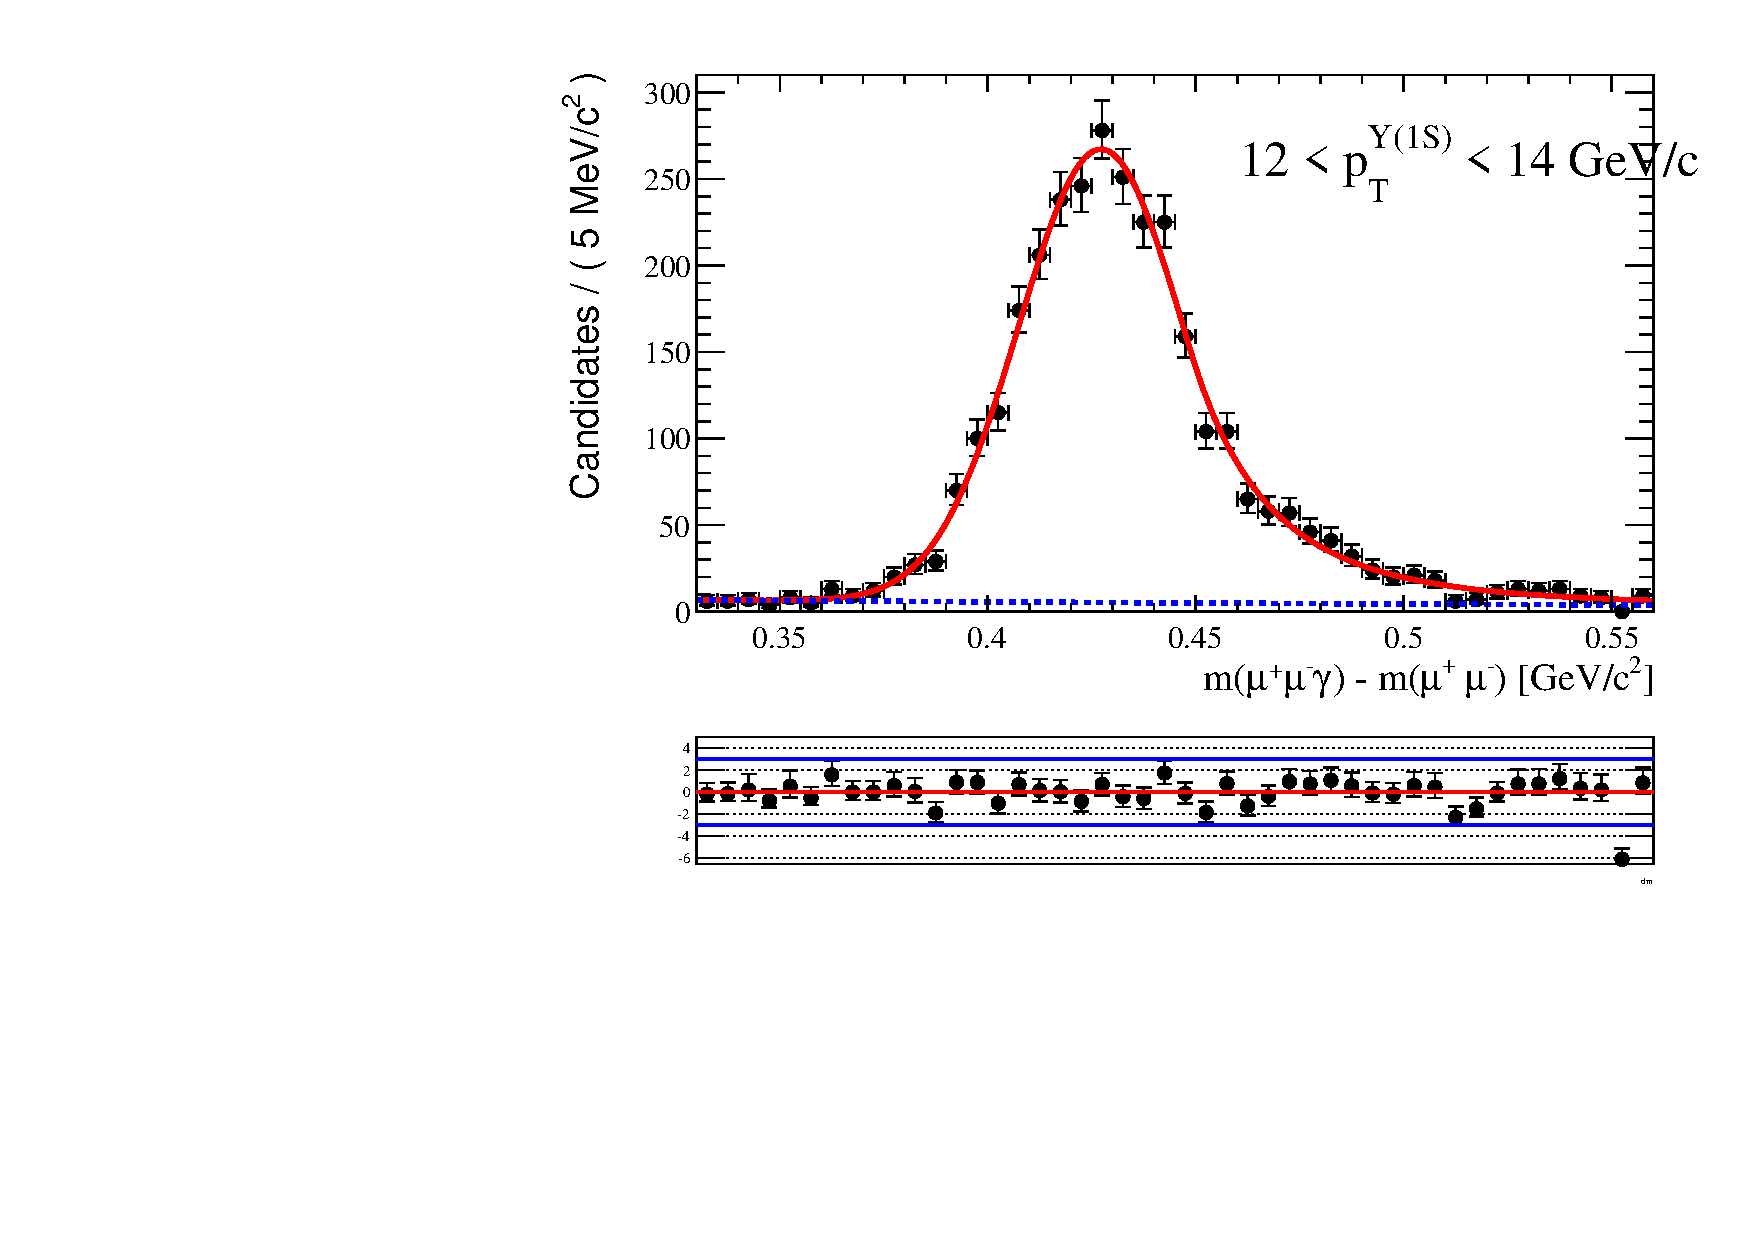
\includegraphics[width=0.16\linewidth]{fit_mc/chib11_12_14}
      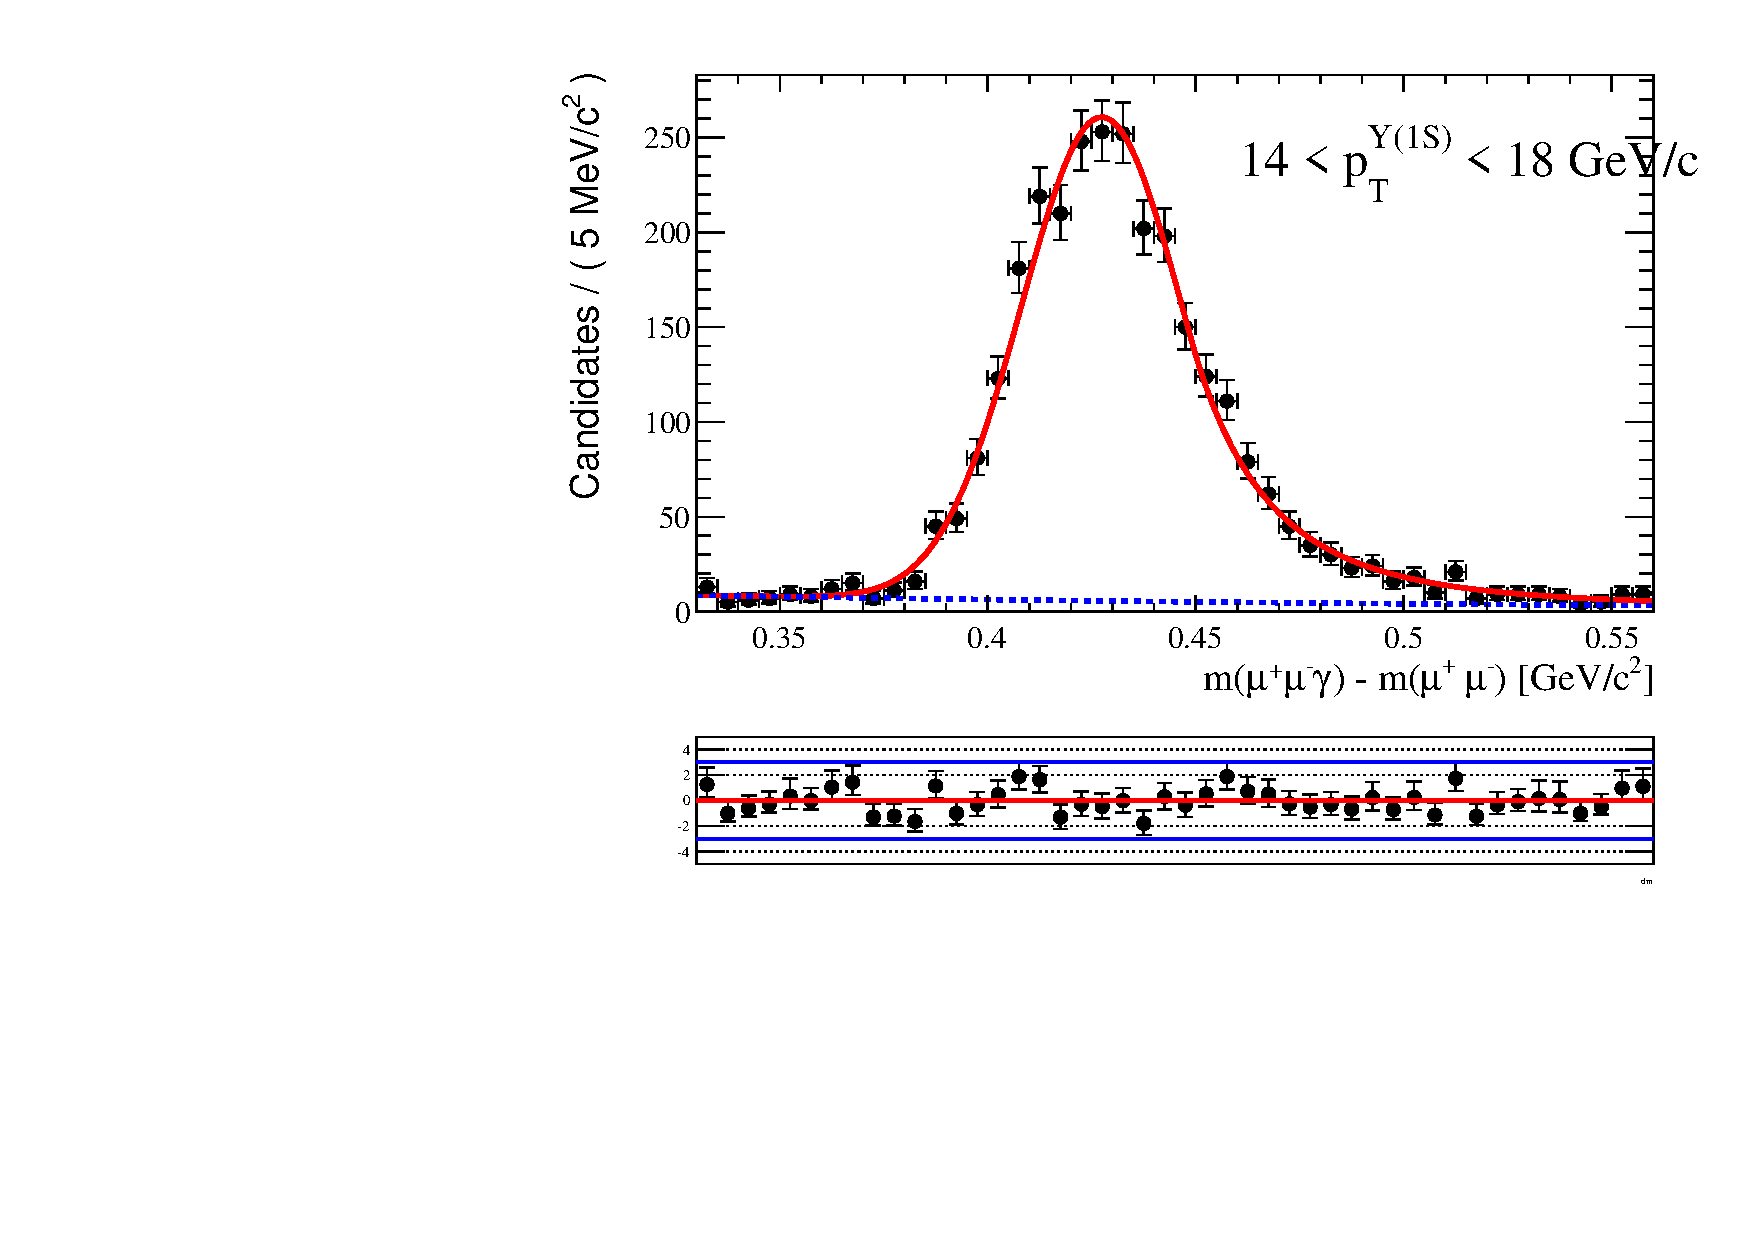
\includegraphics[width=0.16\linewidth]{fit_mc/chib11_14_18}
      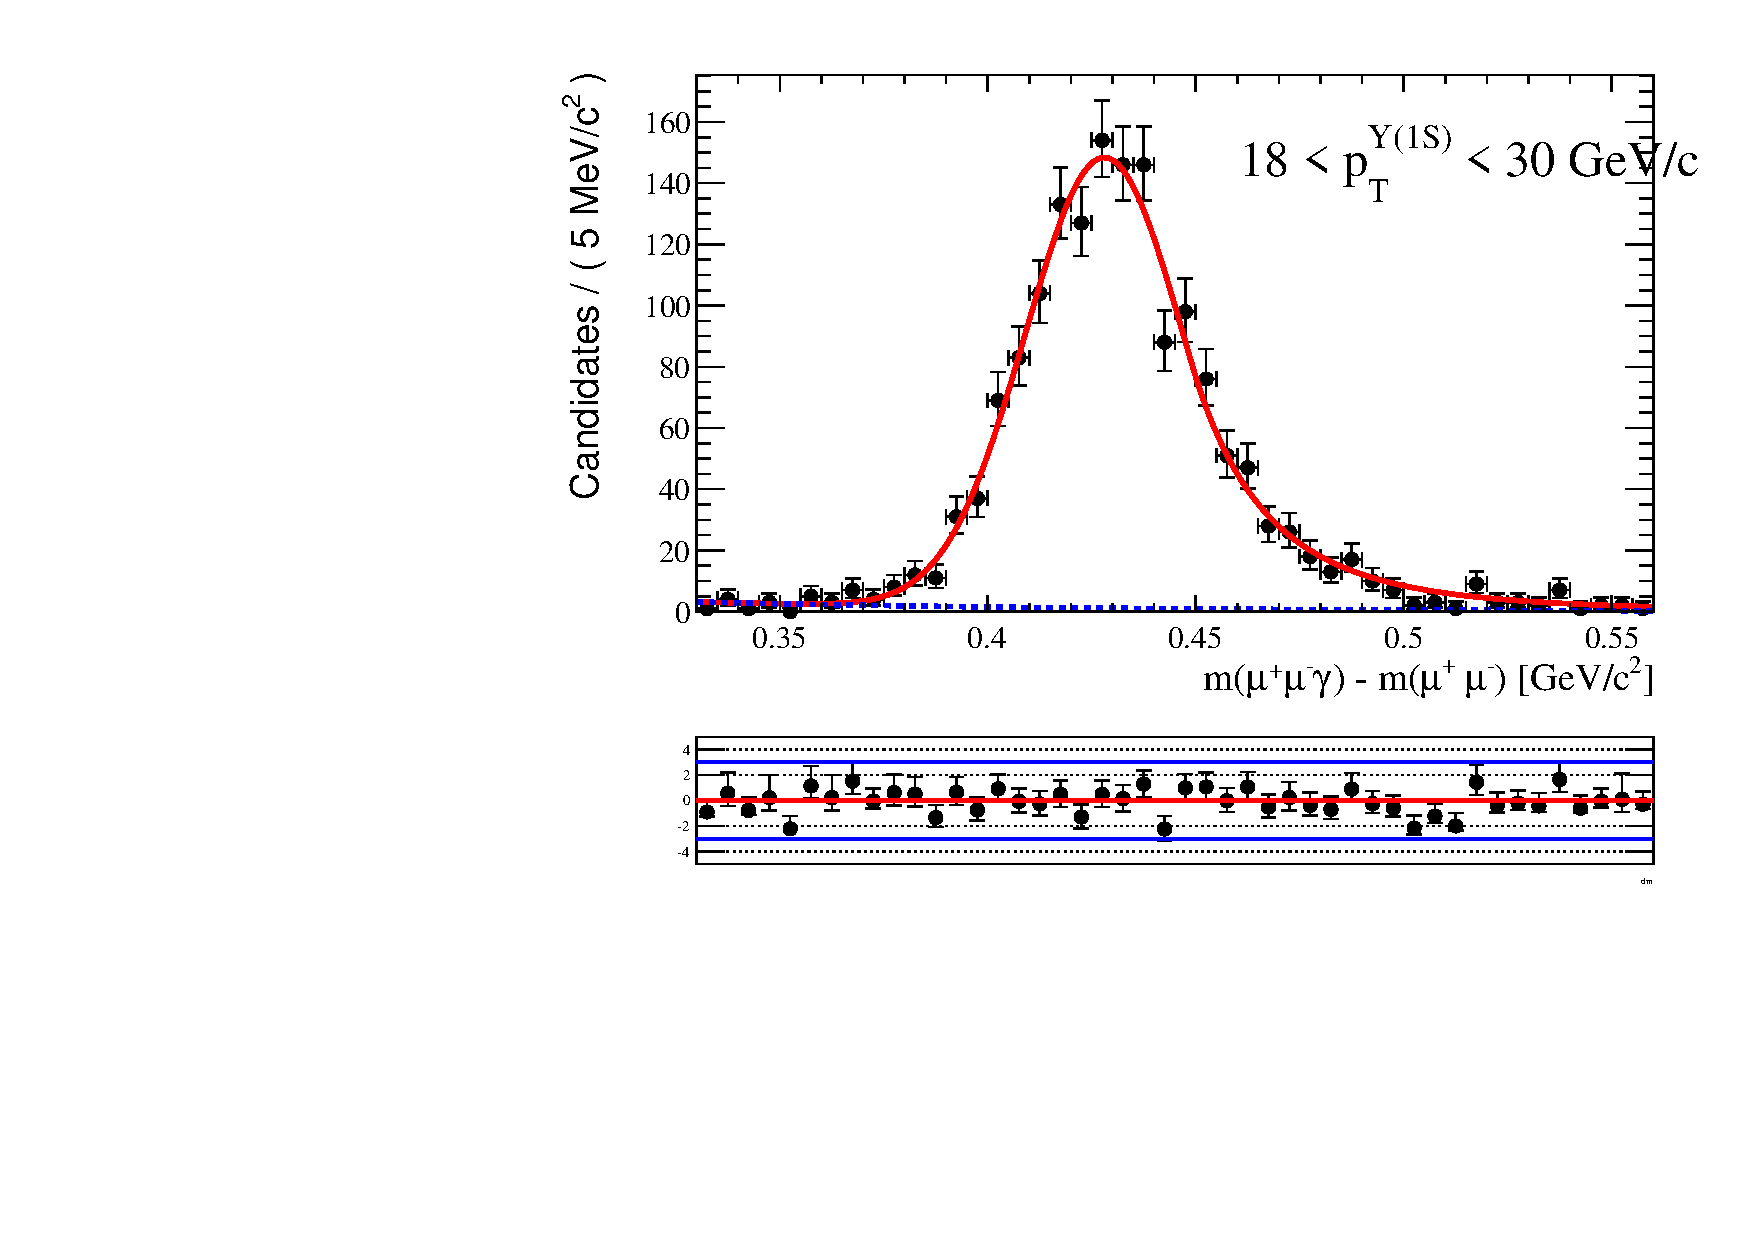
\includegraphics[width=0.16\linewidth]{fit_mc/chib11_18_30}
      \caption{\chiboneOneP}
      \label{fig:fit_mc_chiboneOneP}
    \end{subfigure}
    \begin{subfigure}[b]{\textwidth}
      \centering
      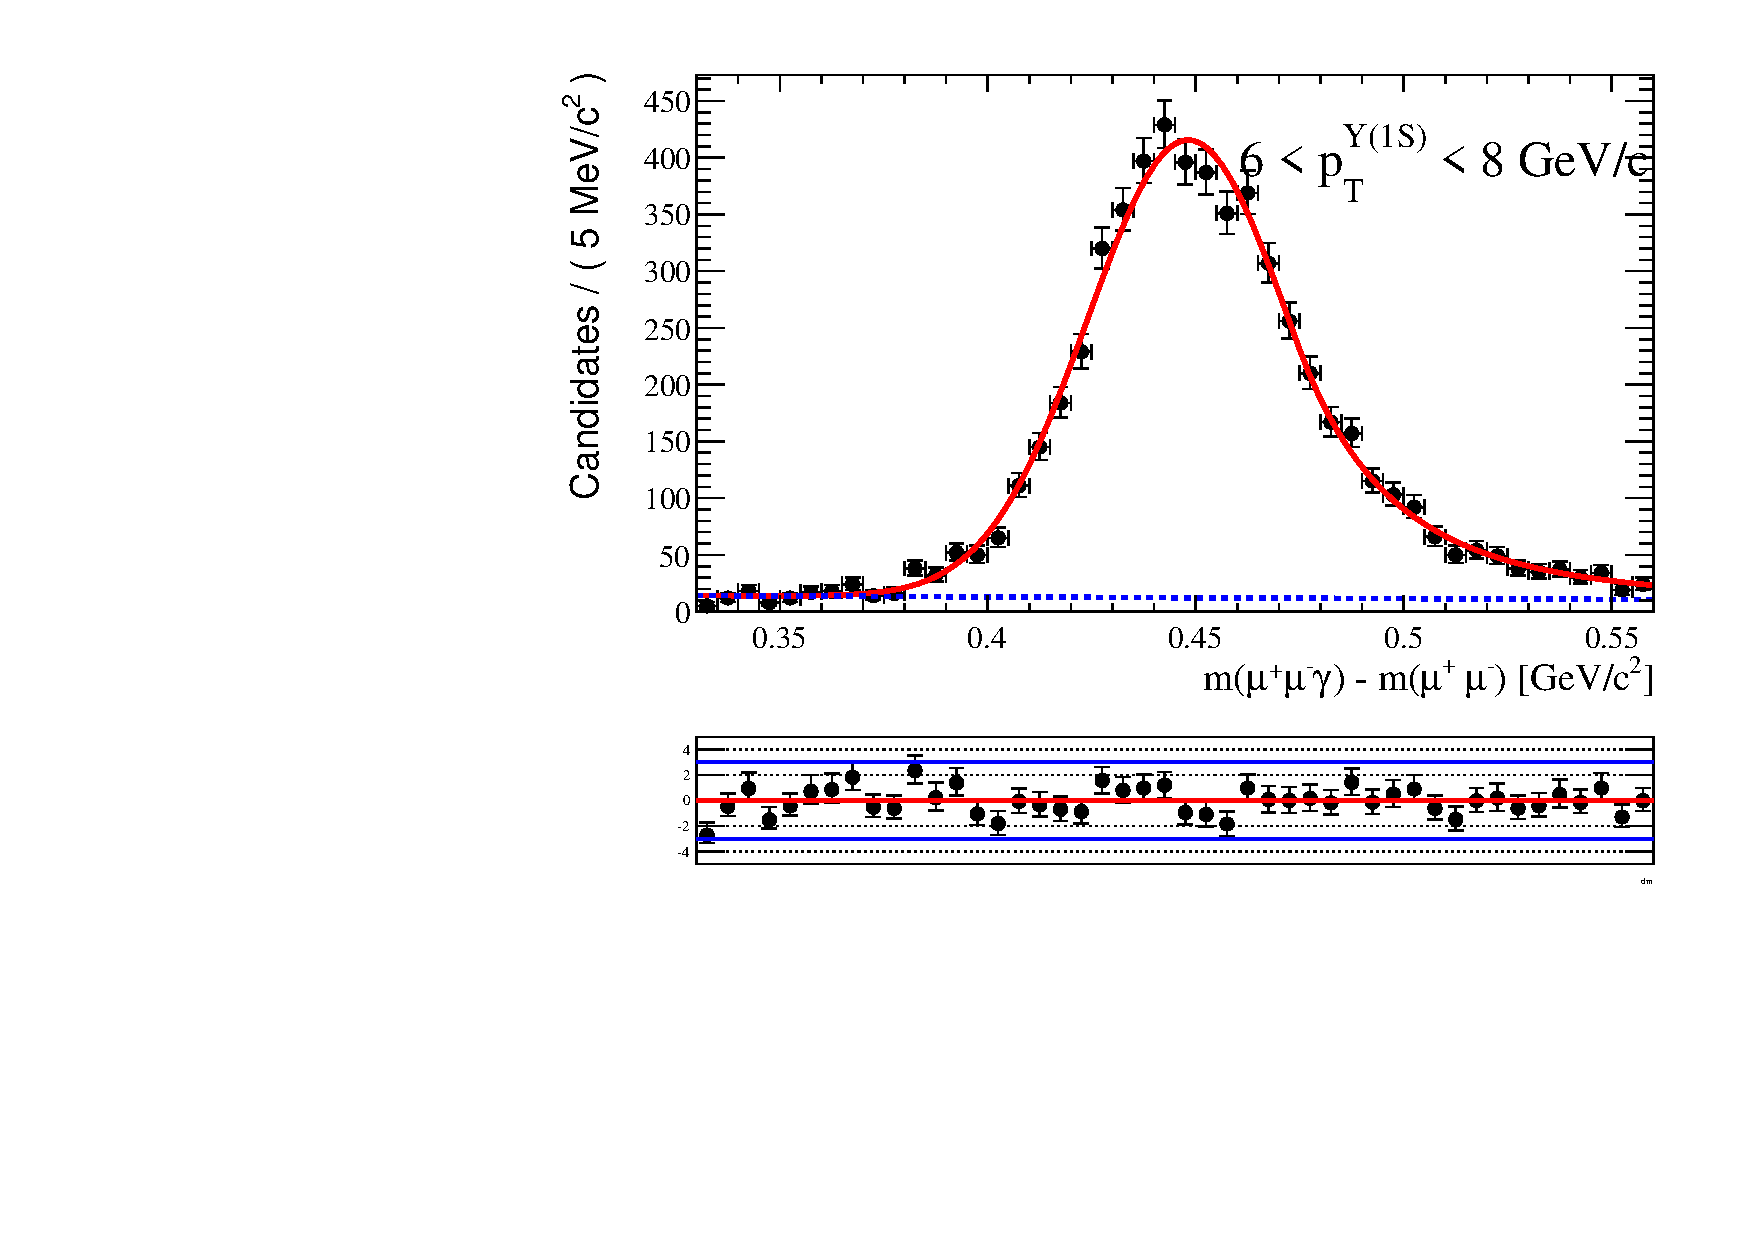
\includegraphics[width=0.16\linewidth]{fit_mc/chib21_6_8}
      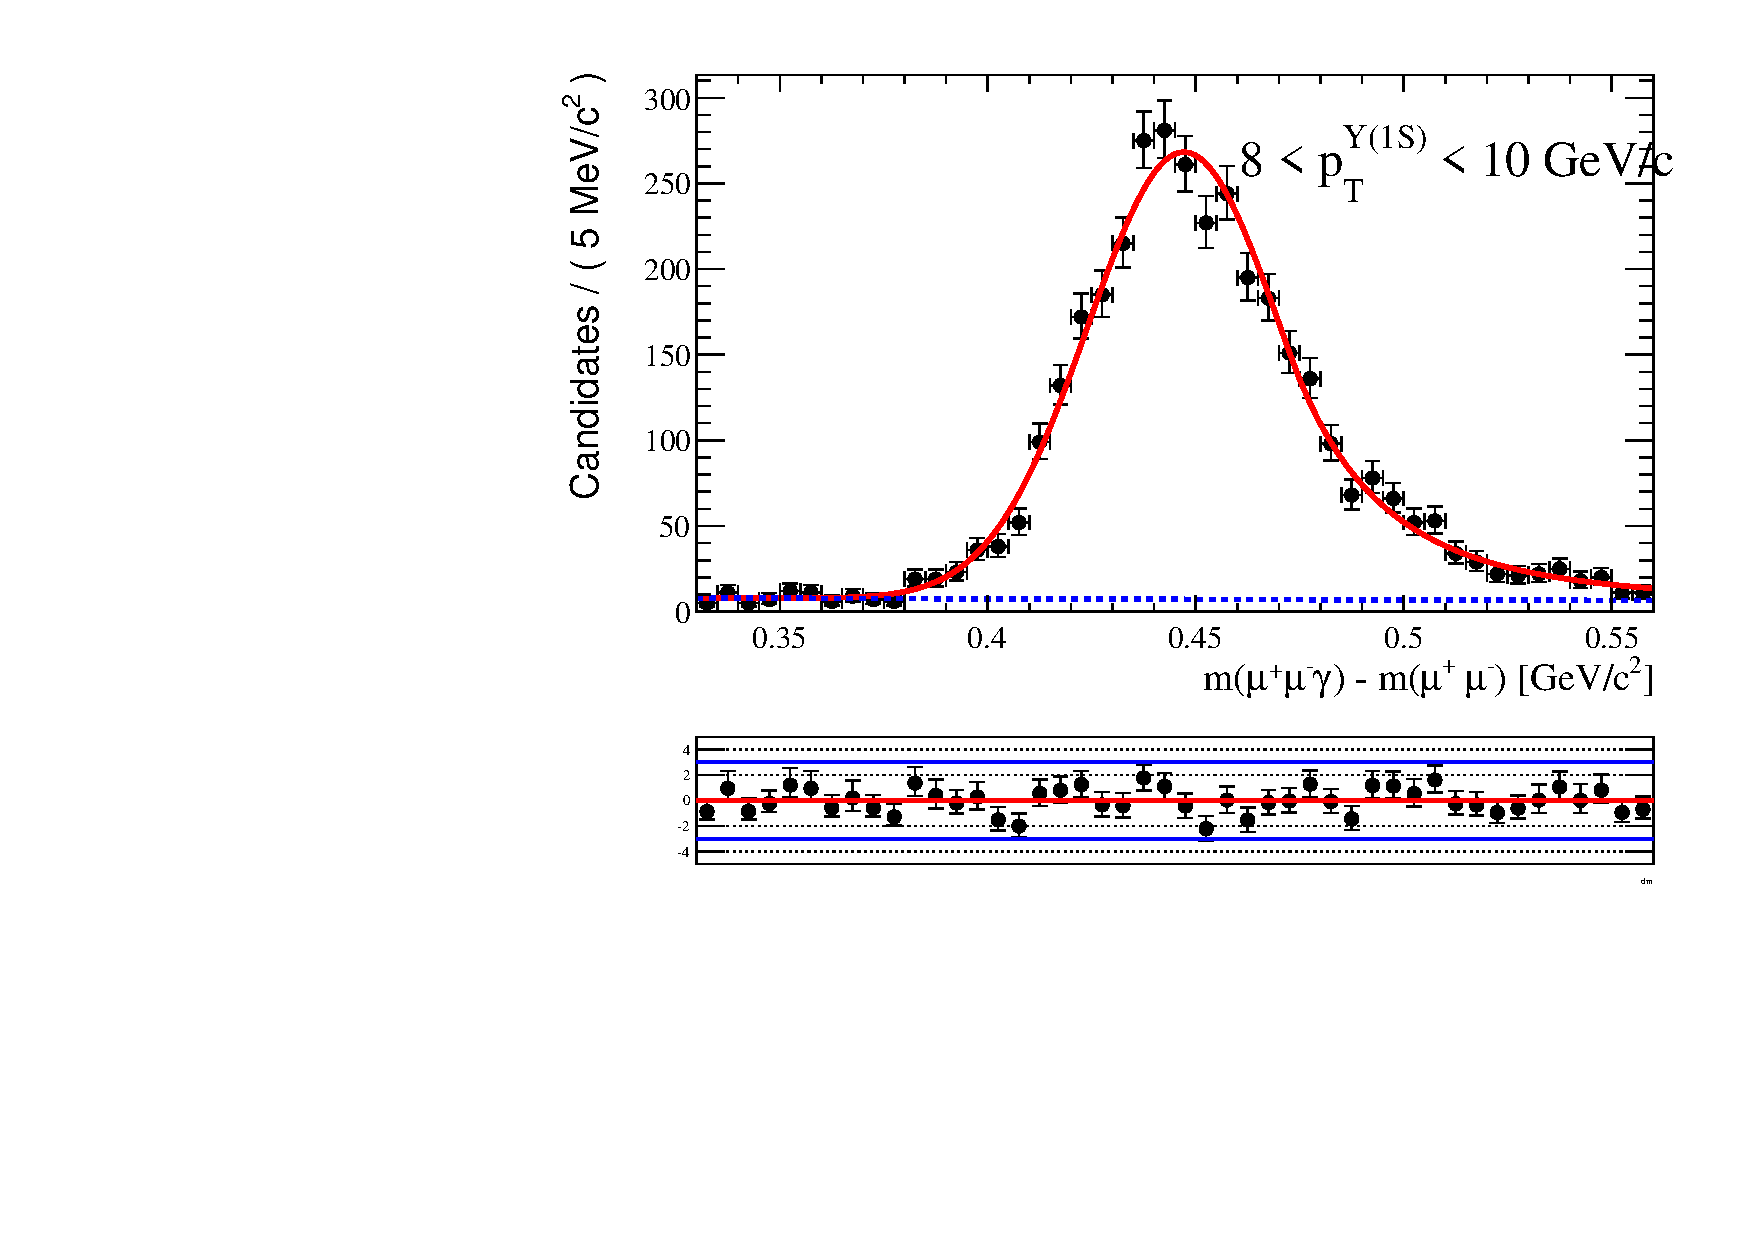
\includegraphics[width=0.16\linewidth]{fit_mc/chib21_8_10}
      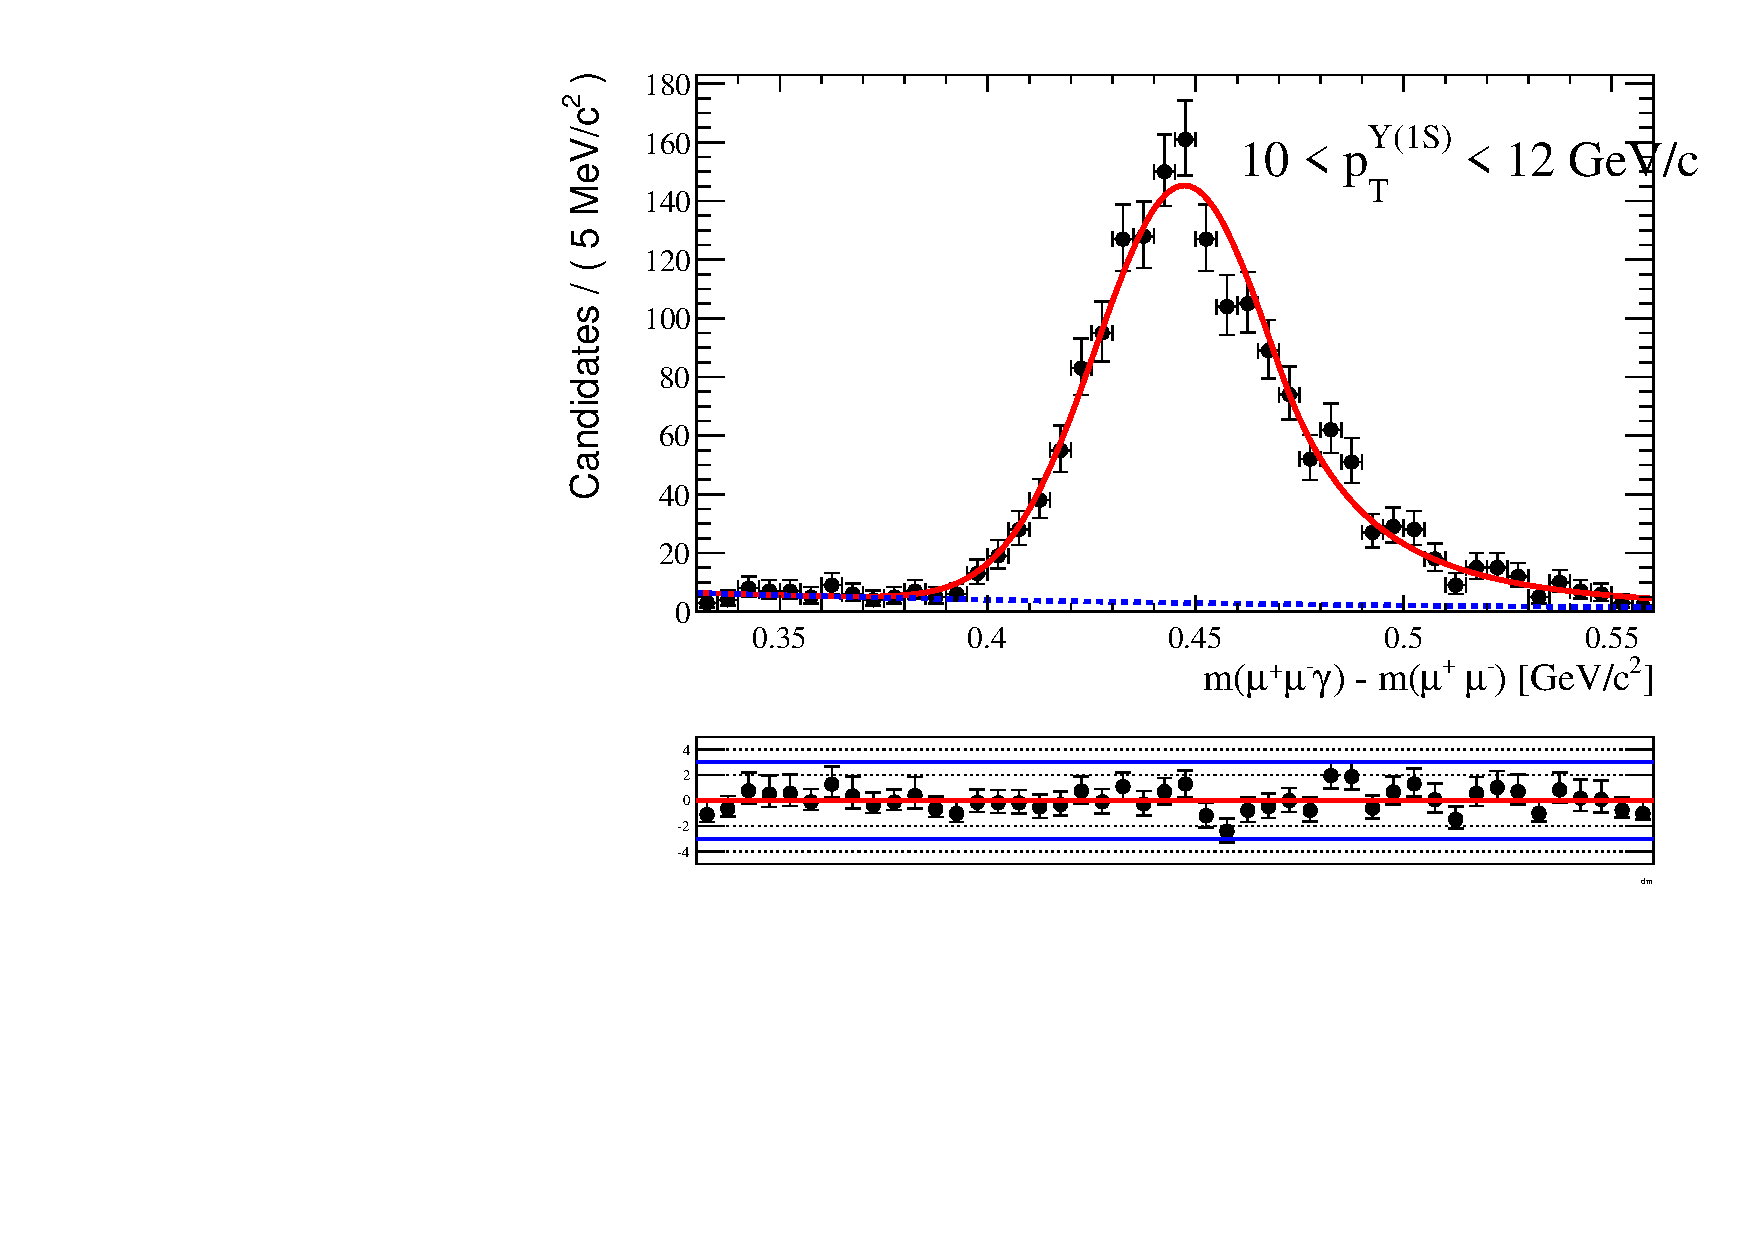
\includegraphics[width=0.16\linewidth]{fit_mc/chib21_10_12}
      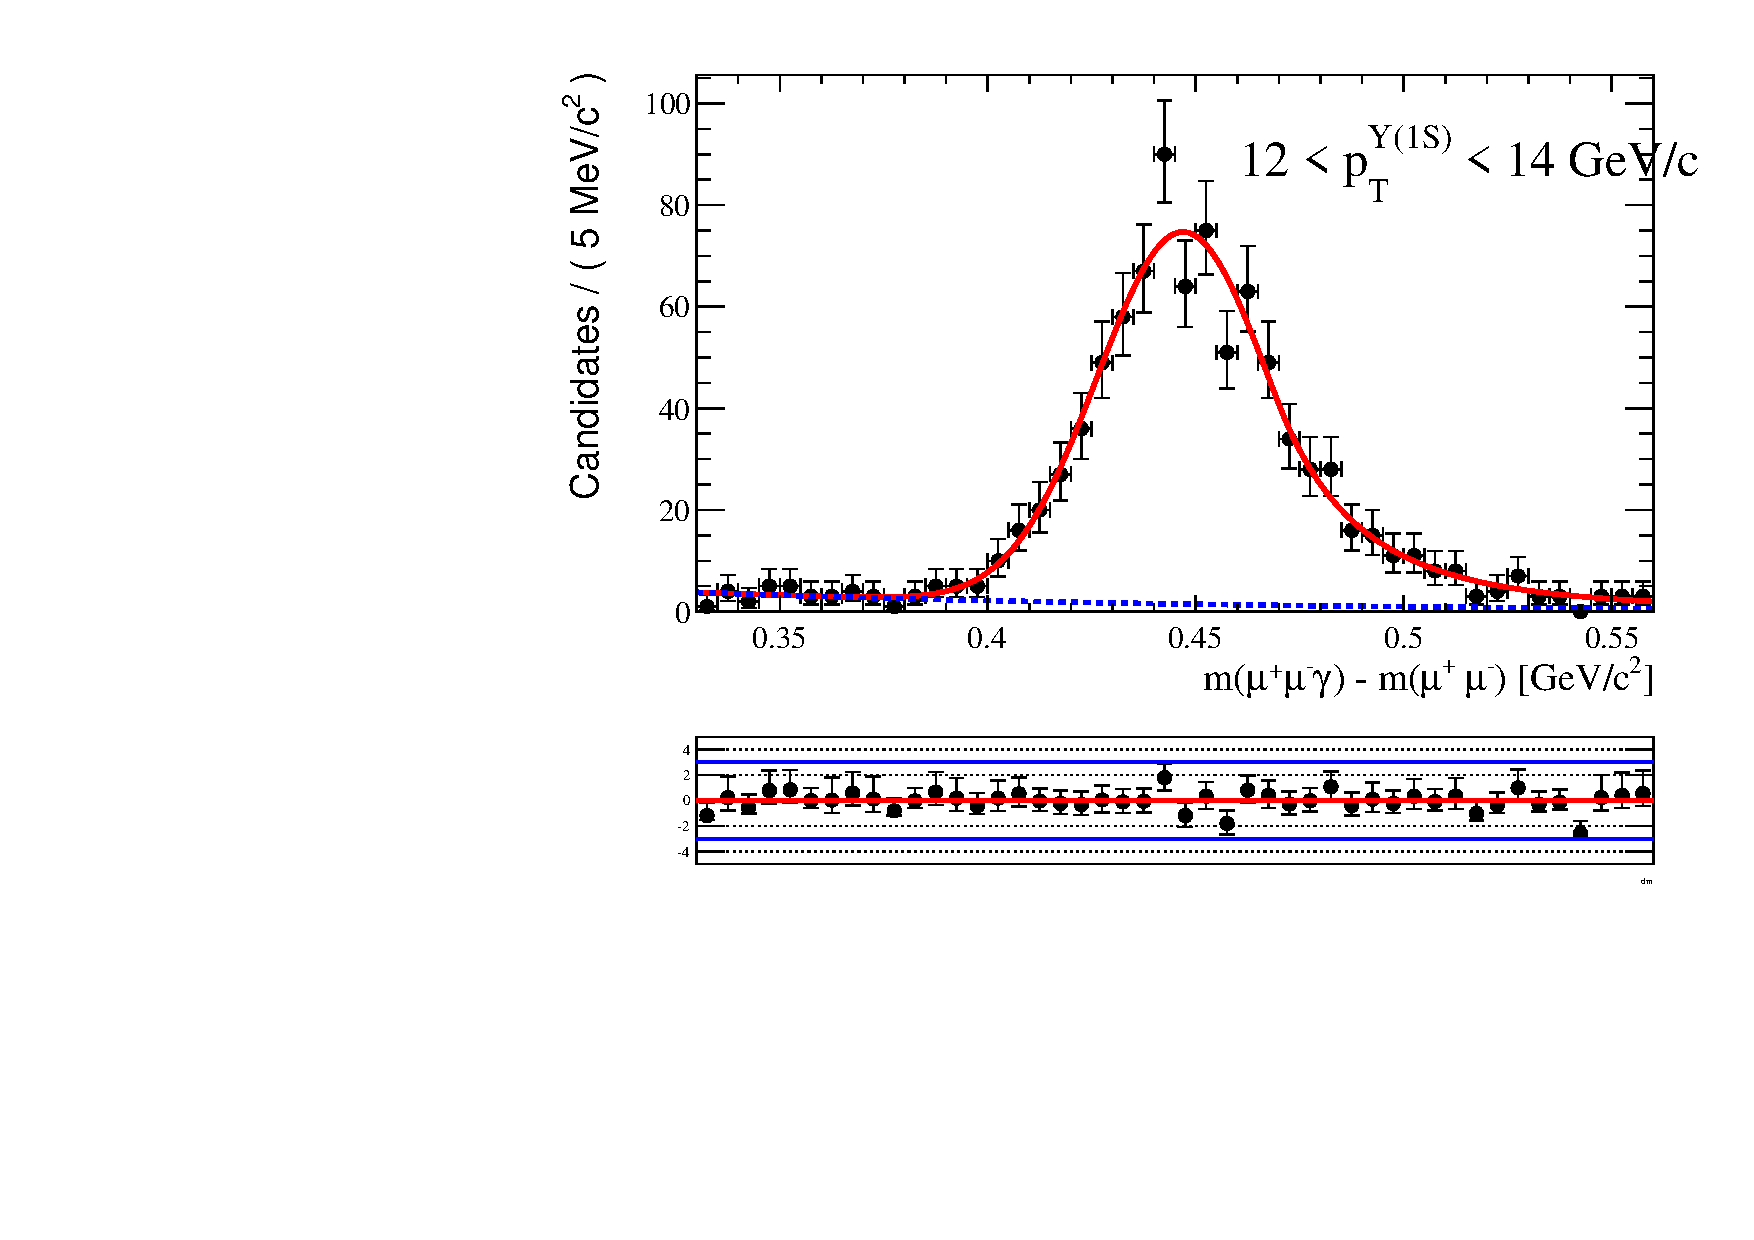
\includegraphics[width=0.16\linewidth]{fit_mc/chib21_12_14}
      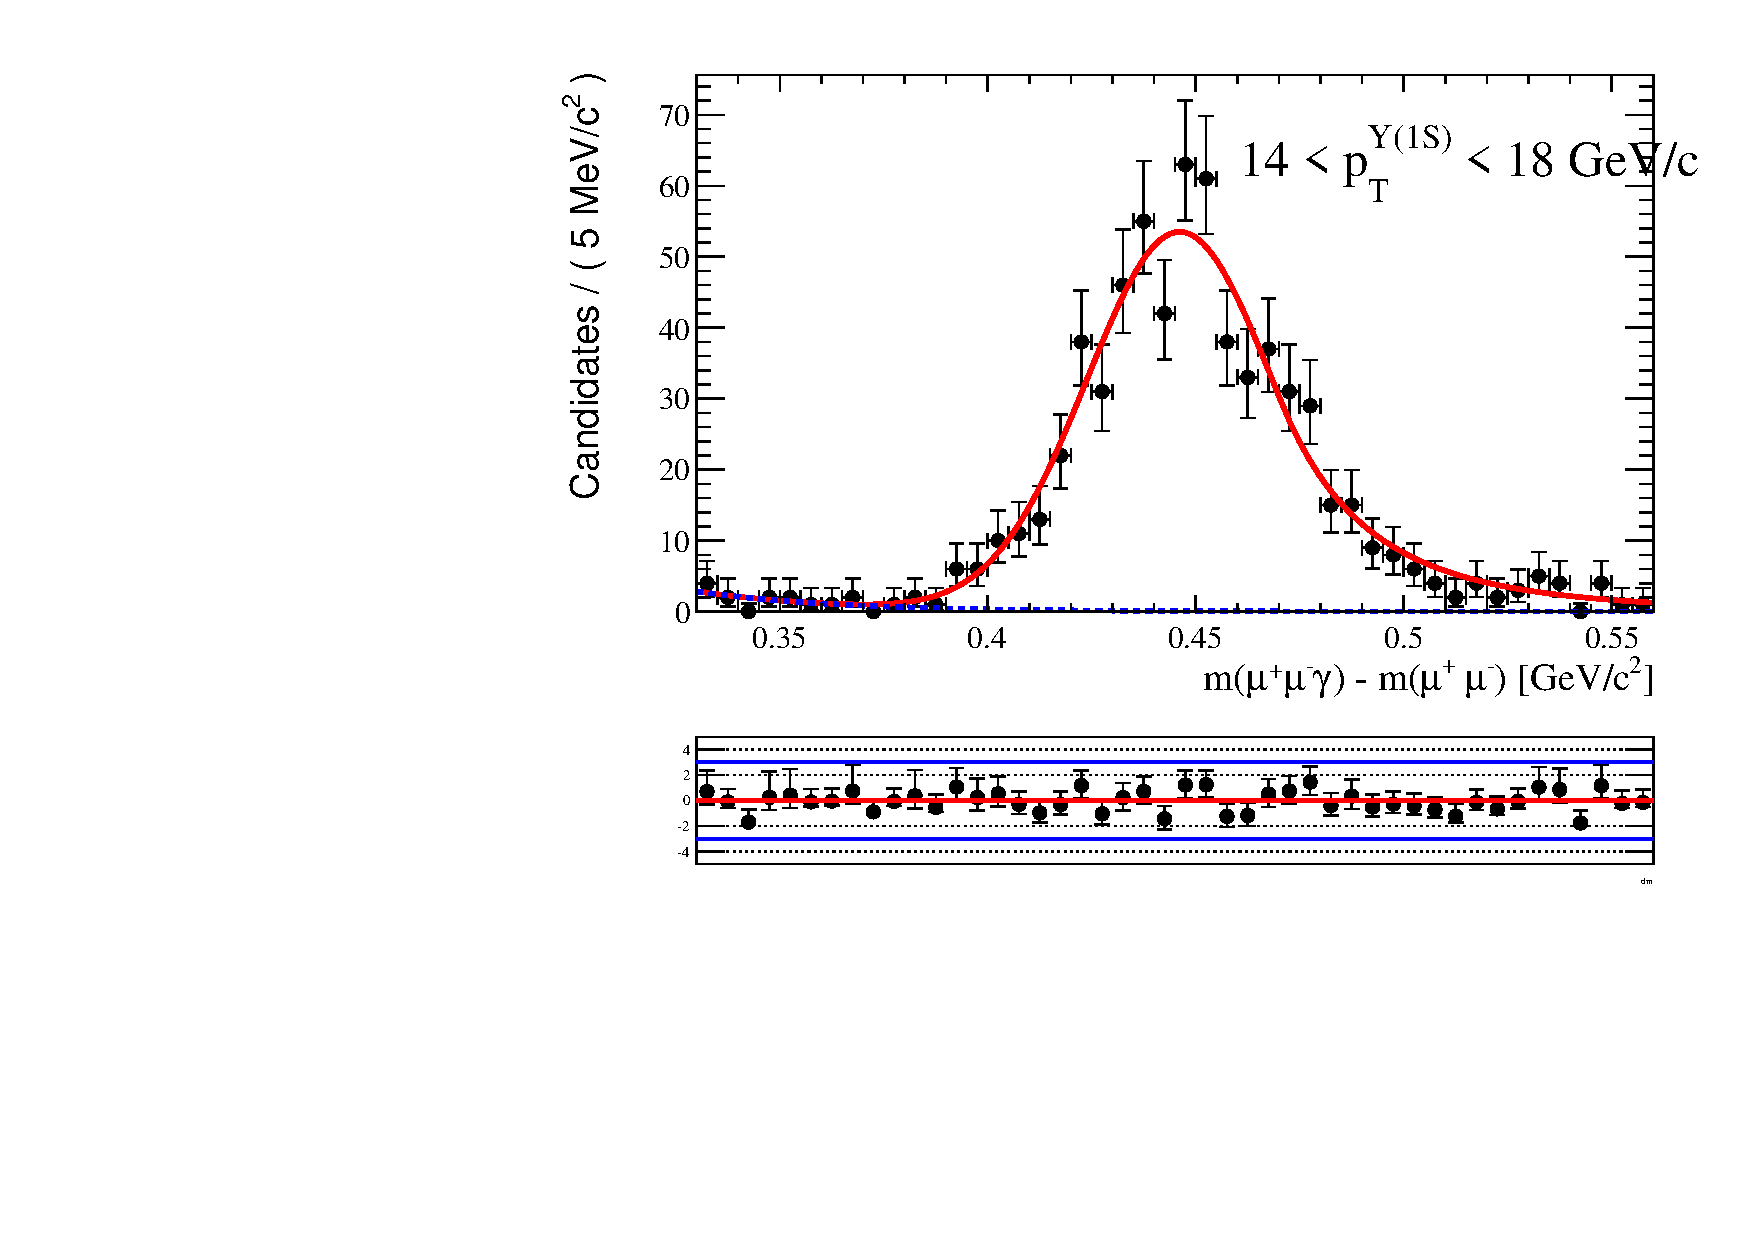
\includegraphics[width=0.16\linewidth]{fit_mc/chib21_14_18}
      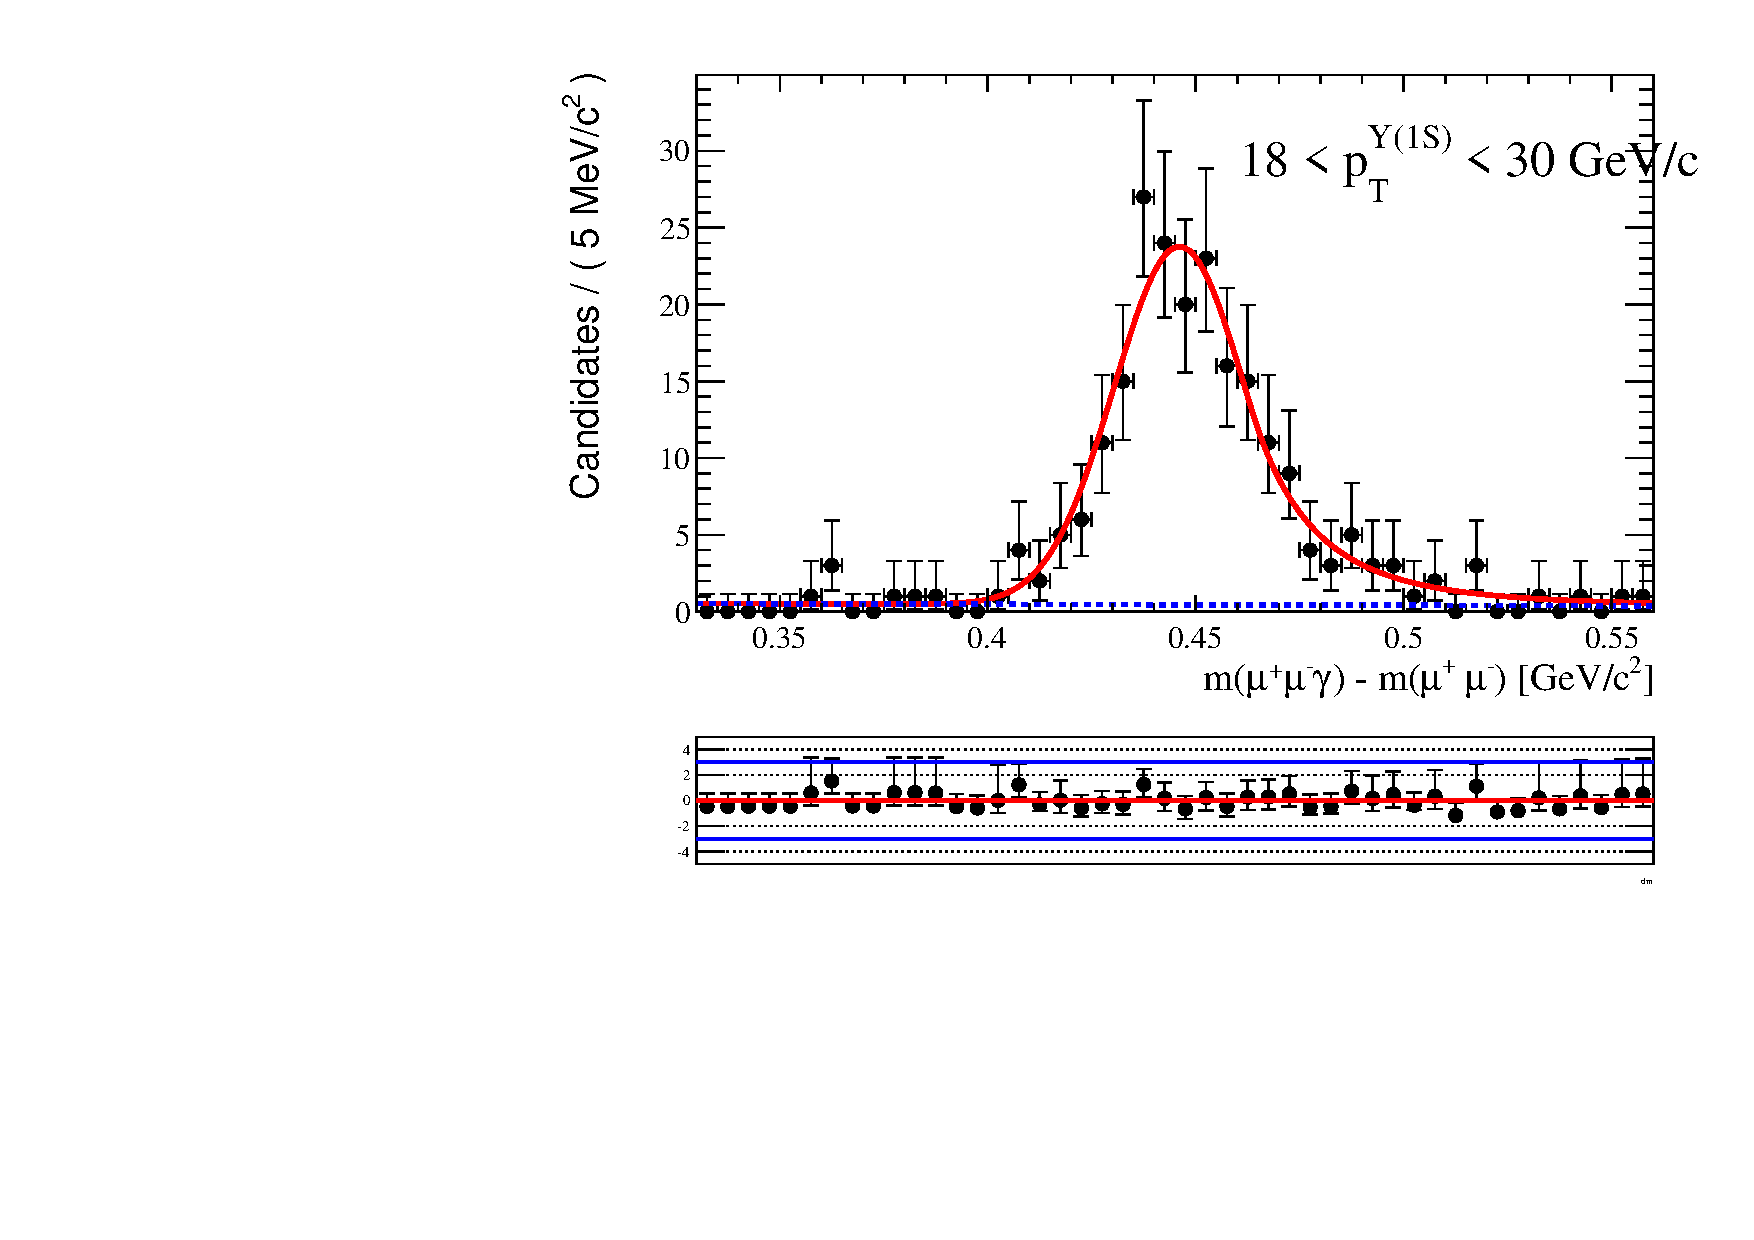
\includegraphics[width=0.16\linewidth]{fit_mc/chib21_18_30}
      \caption{\chibtwoOneP}
      \label{fig:fit_mc_chibtwoOneP}
    \end{subfigure}
    \begin{subfigure}[b]{\textwidth}
      \centering
      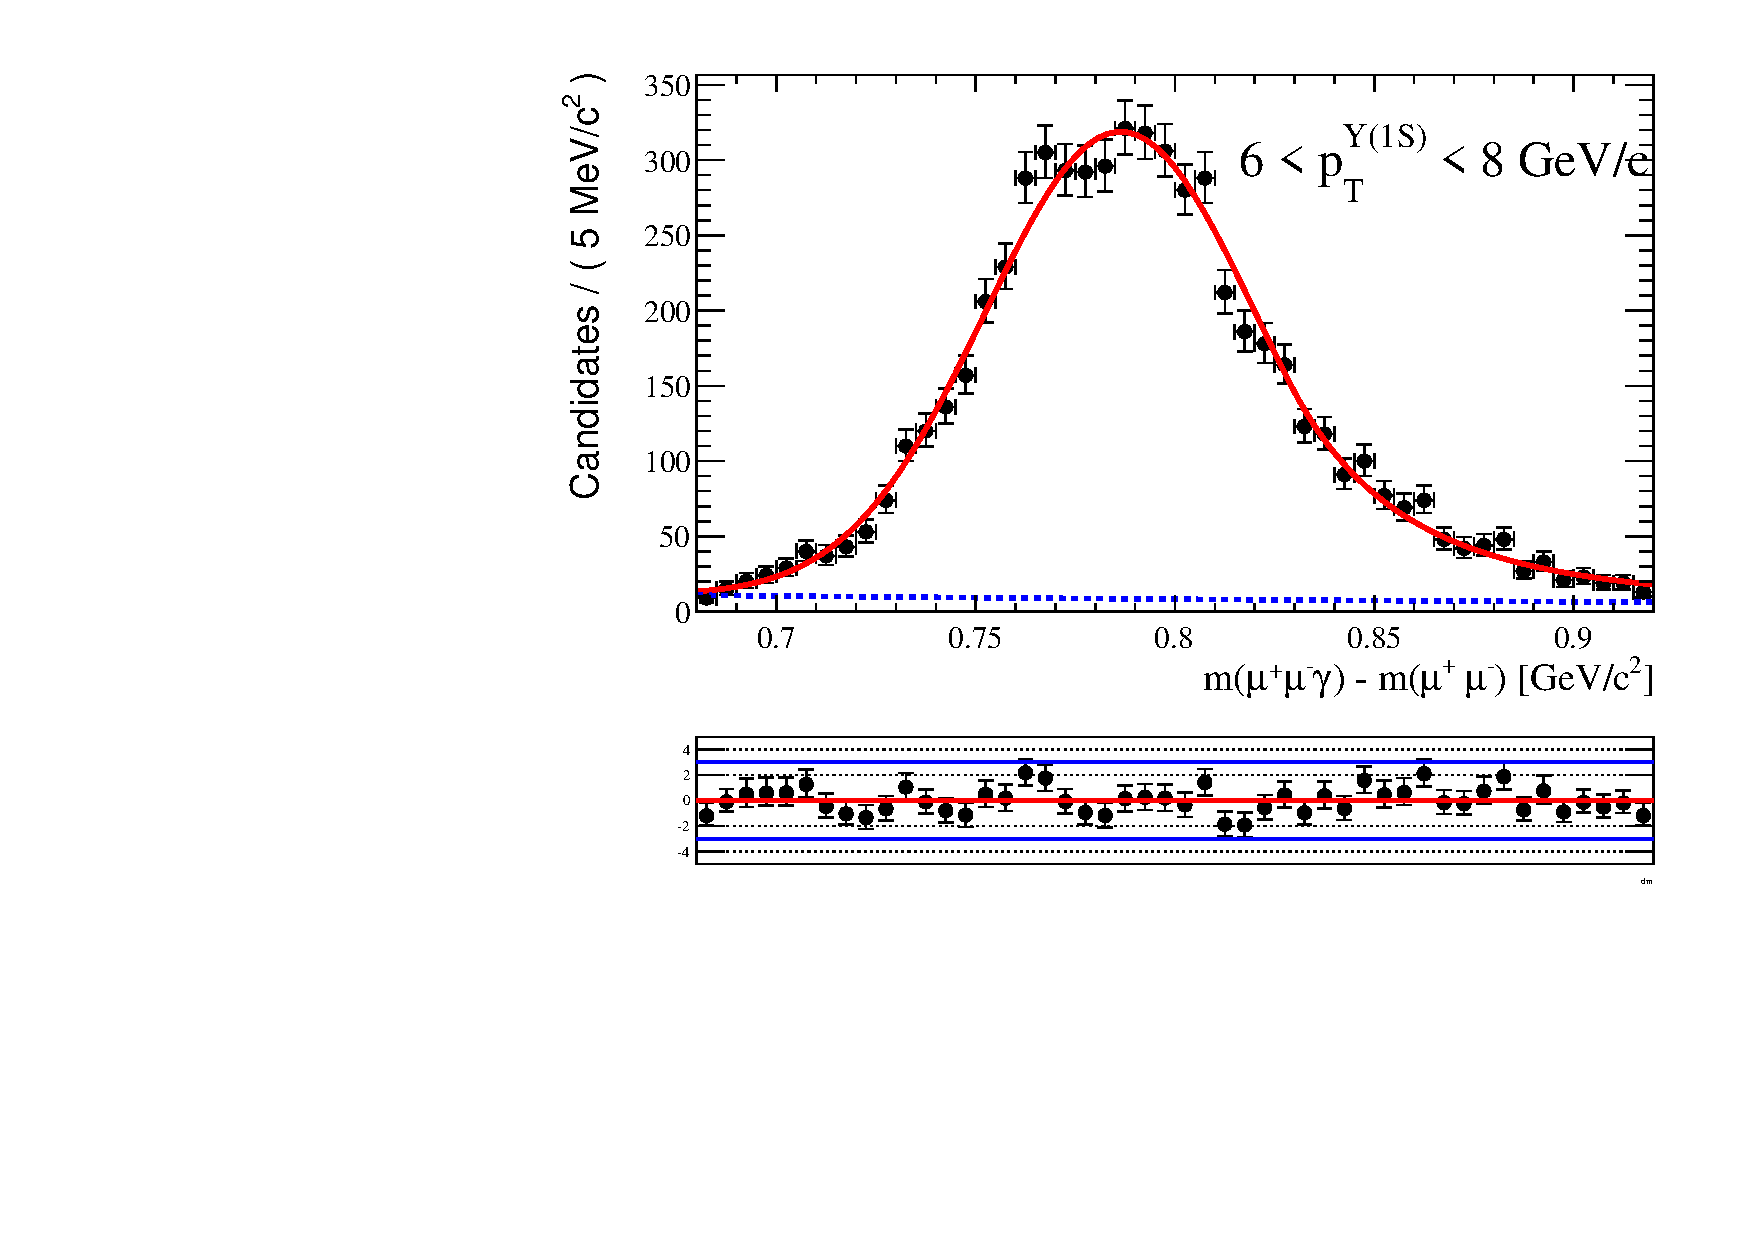
\includegraphics[width=0.16\linewidth]{fit_mc/chib12_6_8}
      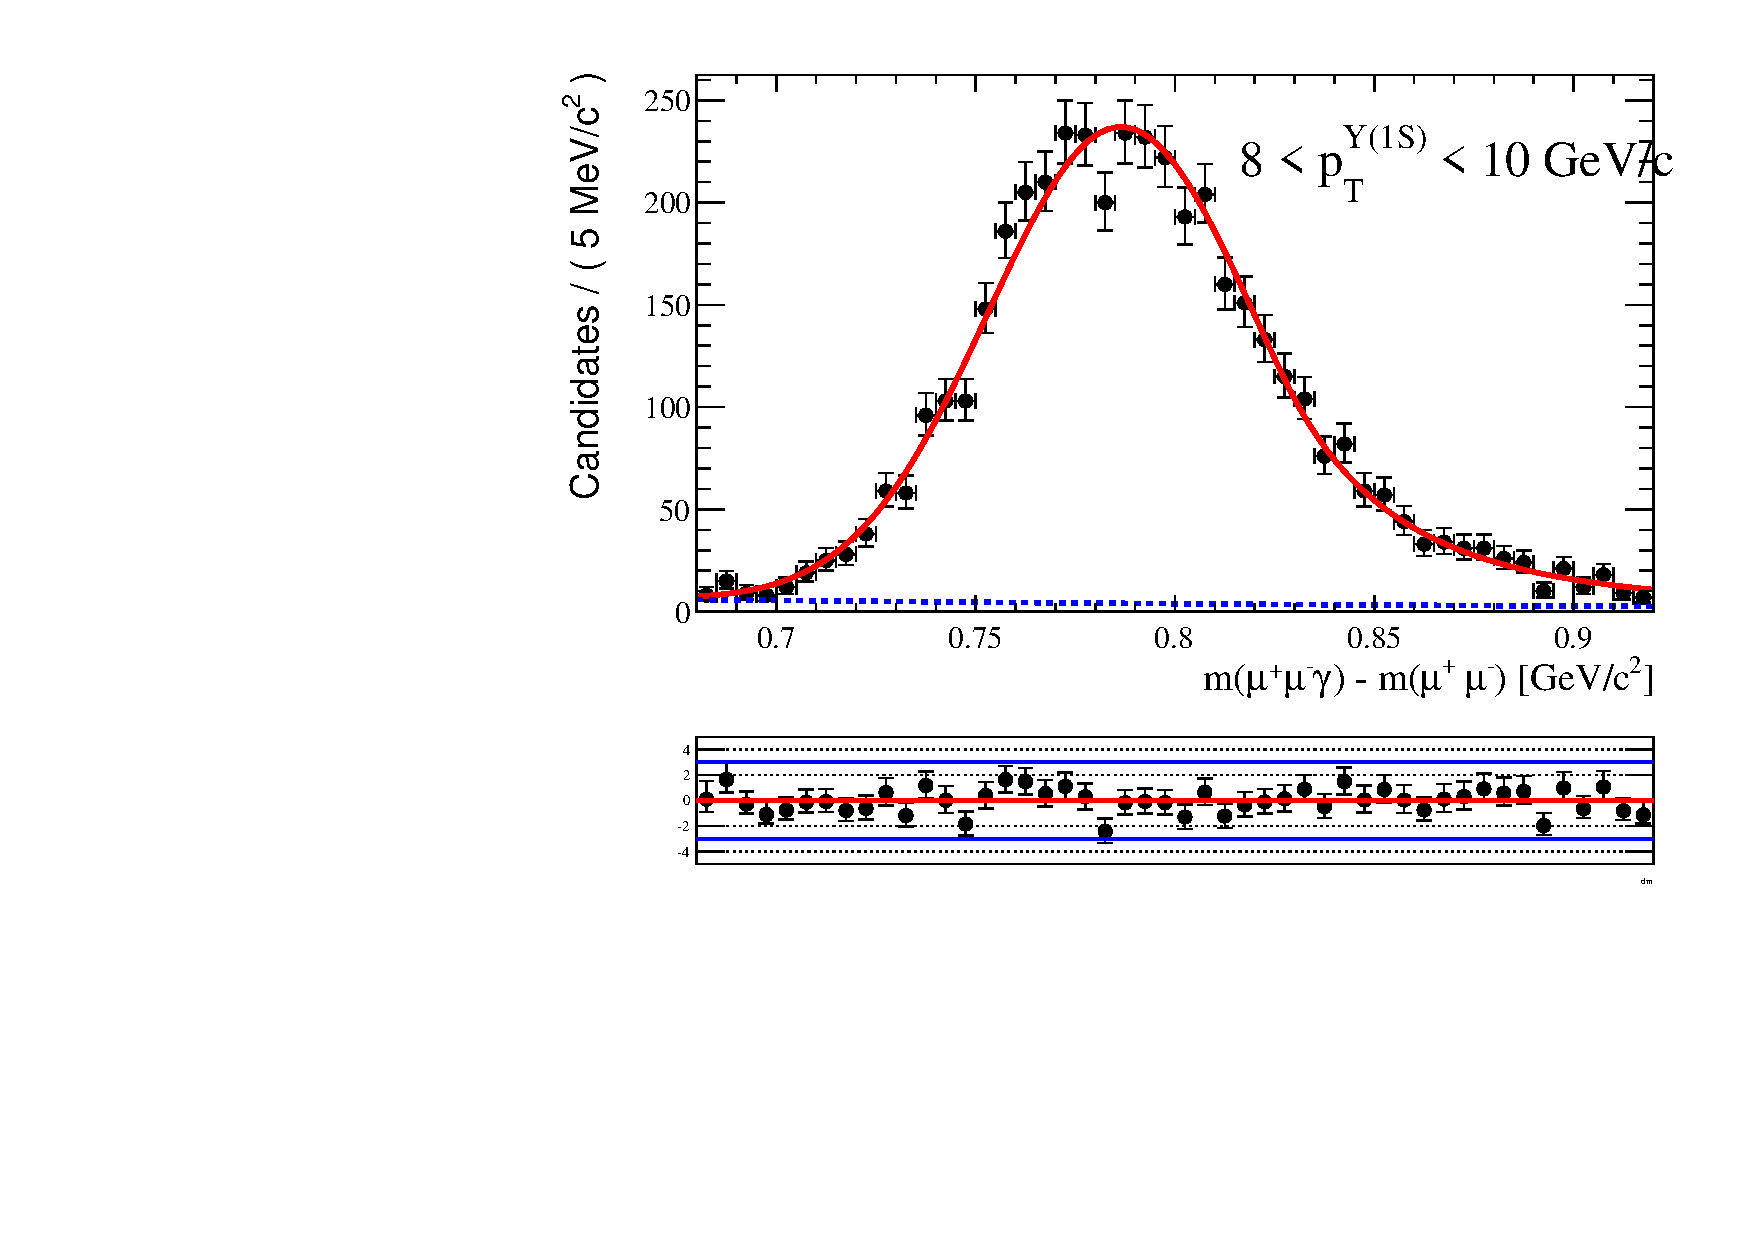
\includegraphics[width=0.16\linewidth]{fit_mc/chib12_8_10}
      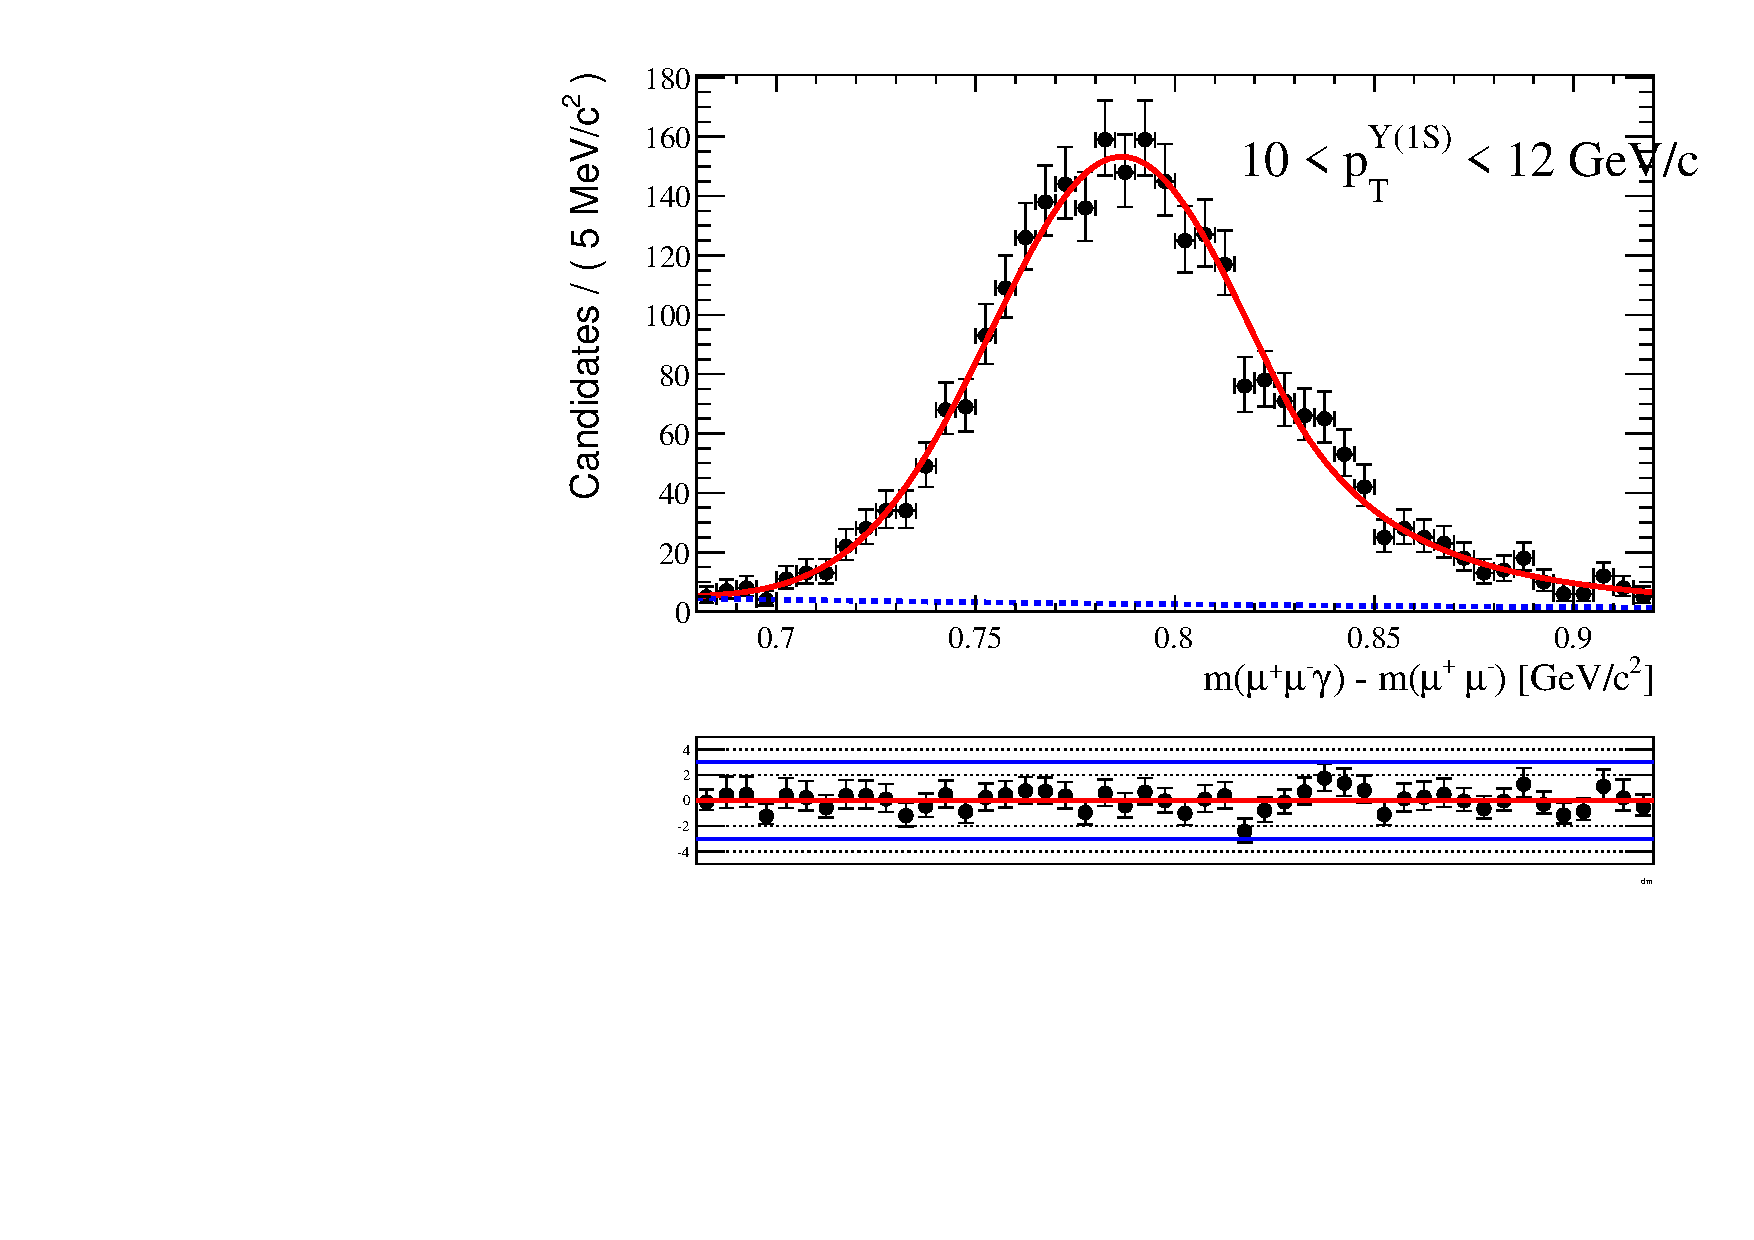
\includegraphics[width=0.16\linewidth]{fit_mc/chib12_10_12}
      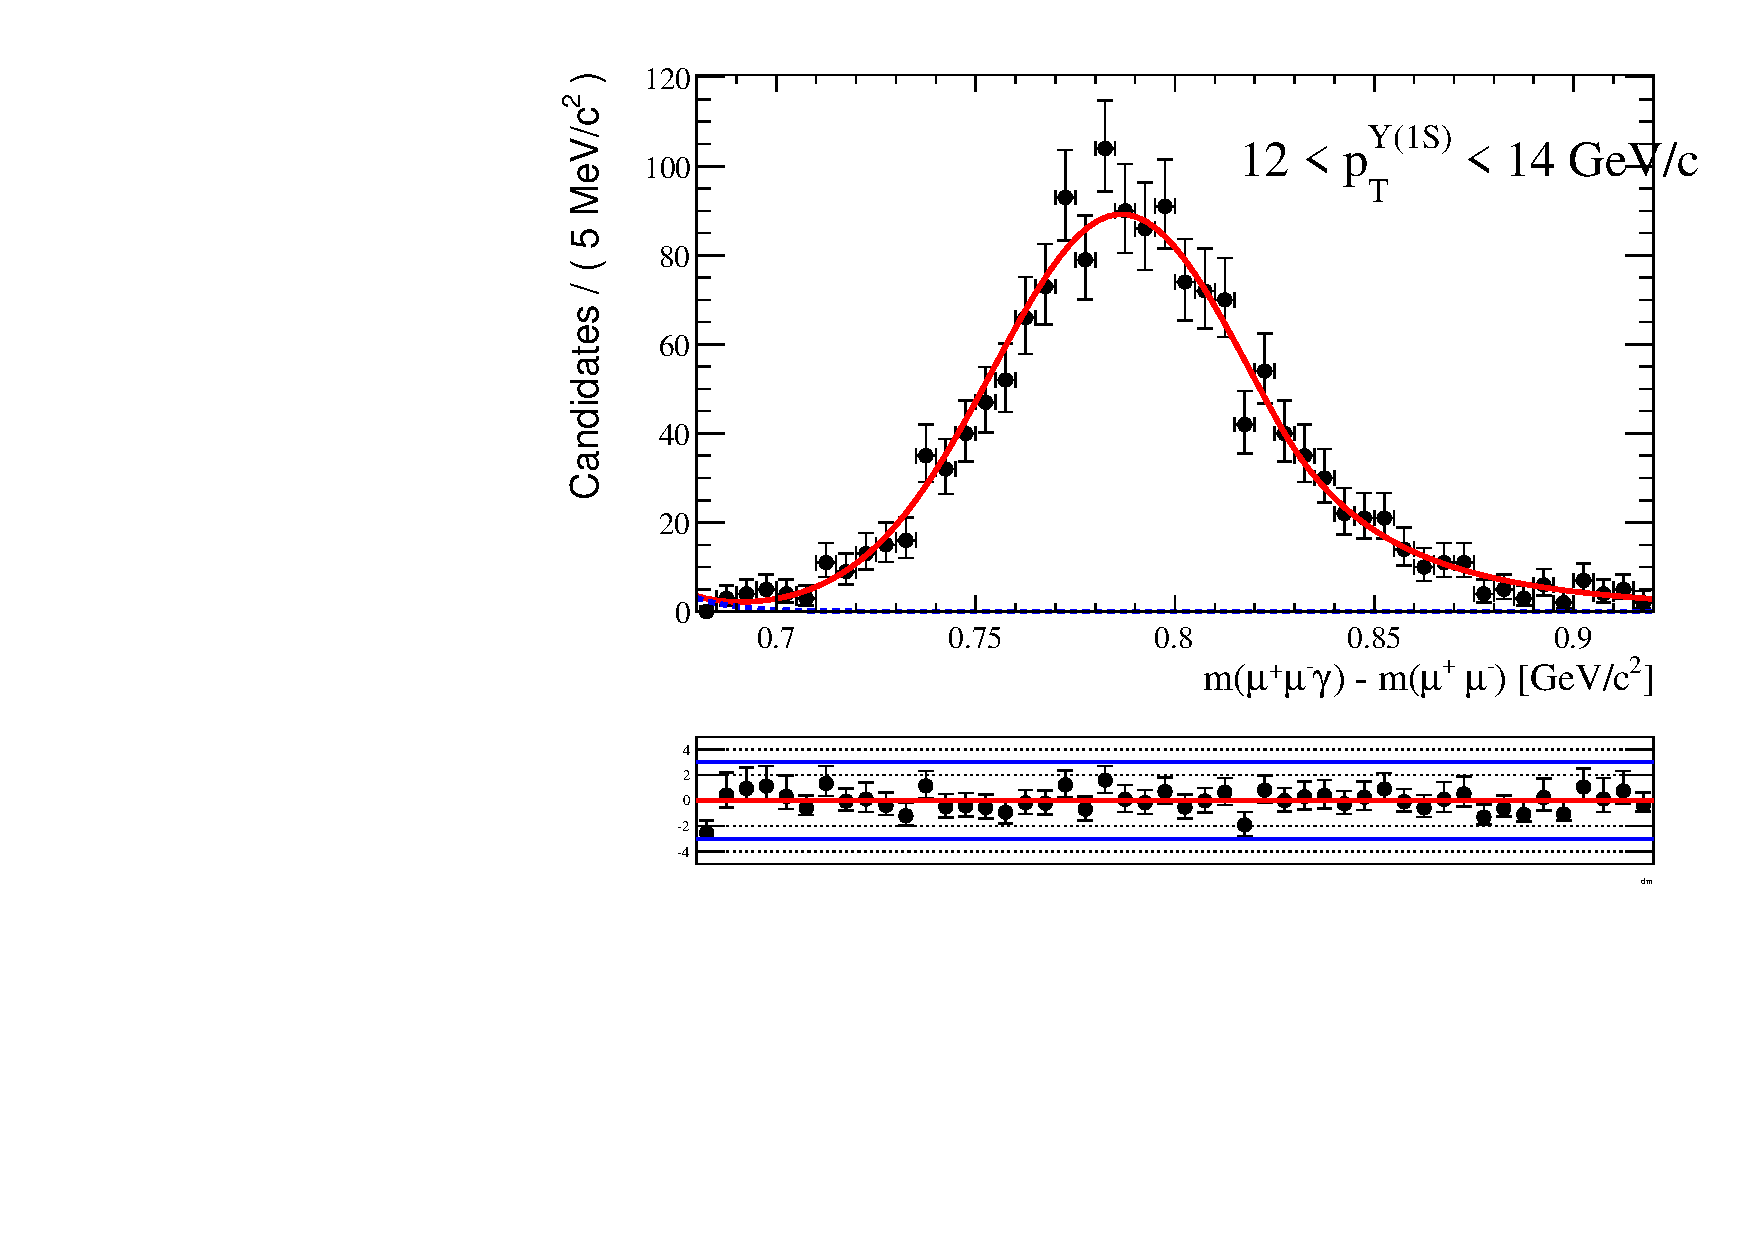
\includegraphics[width=0.16\linewidth]{fit_mc/chib12_12_14}
      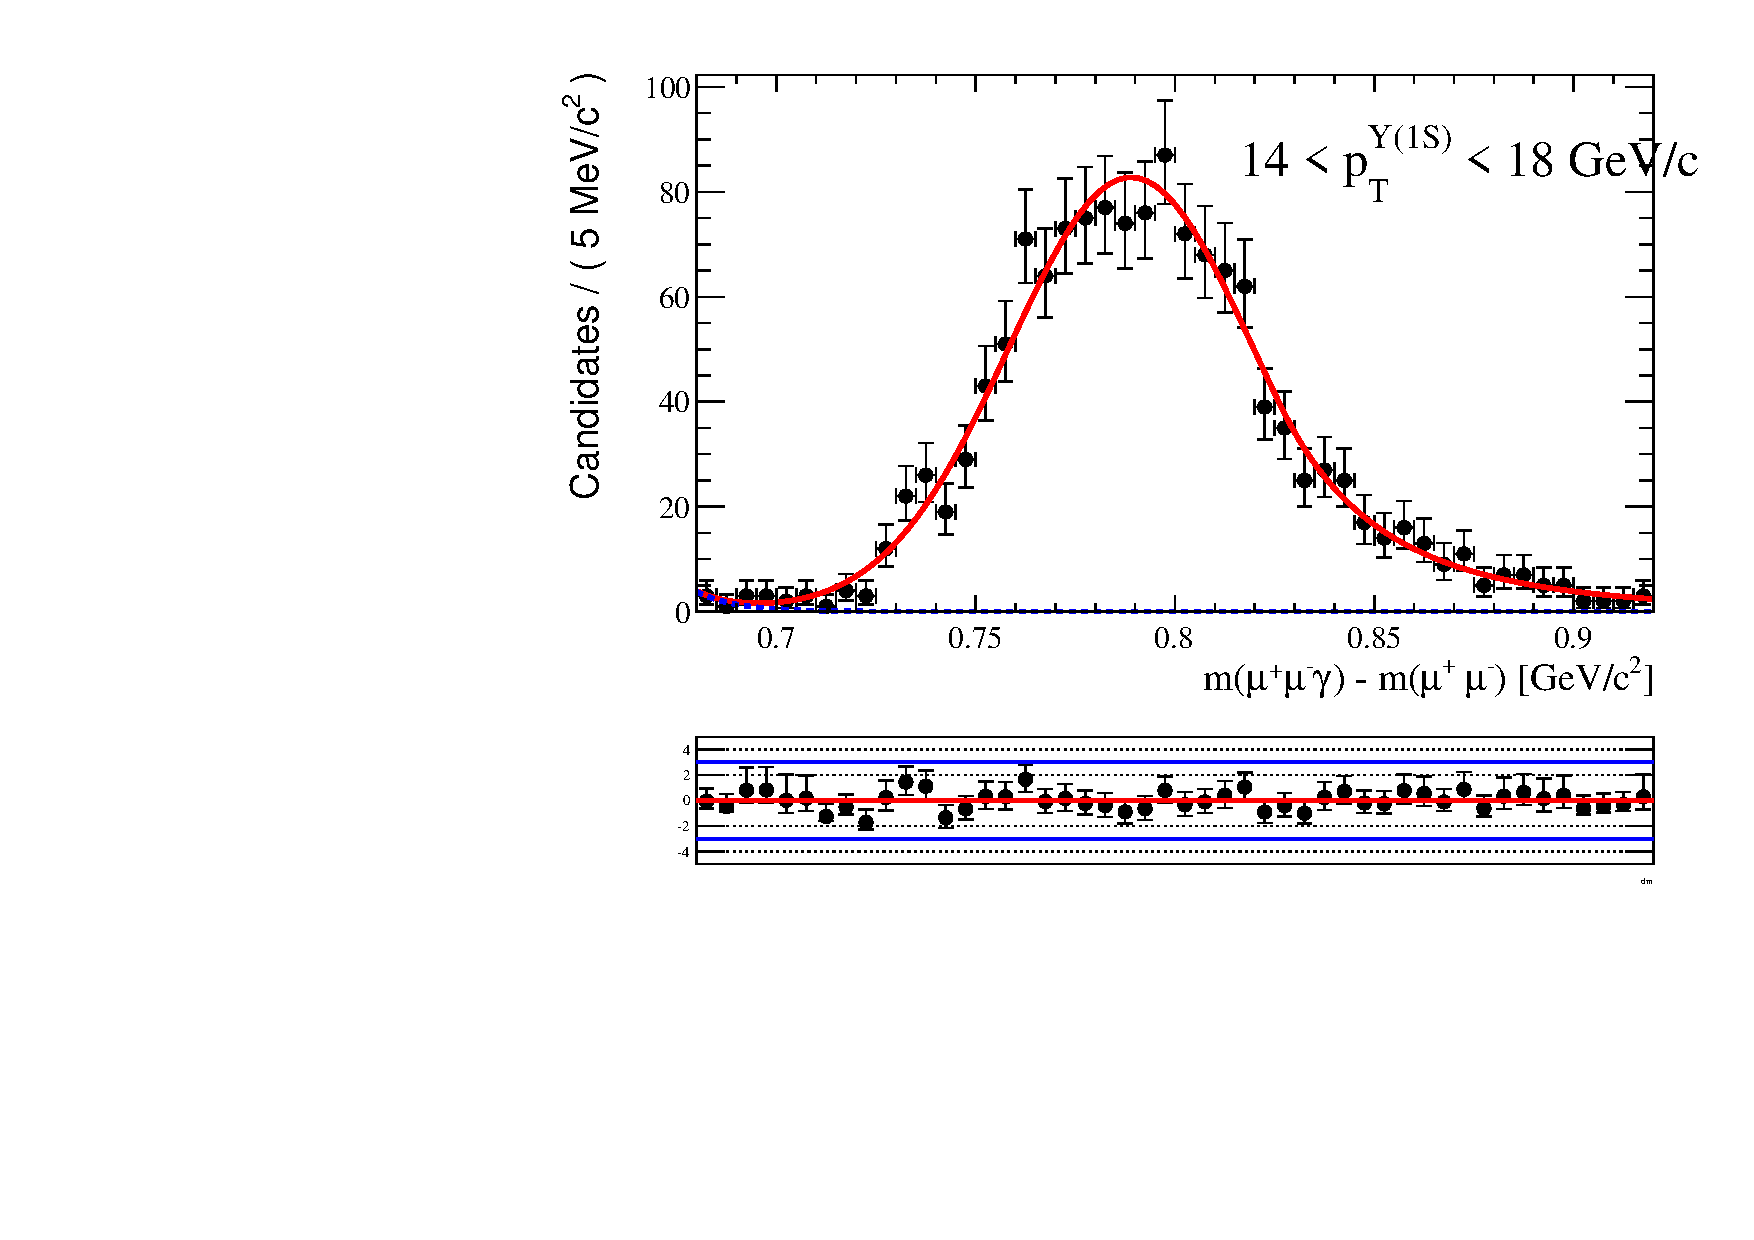
\includegraphics[width=0.16\linewidth]{fit_mc/chib12_14_18}
      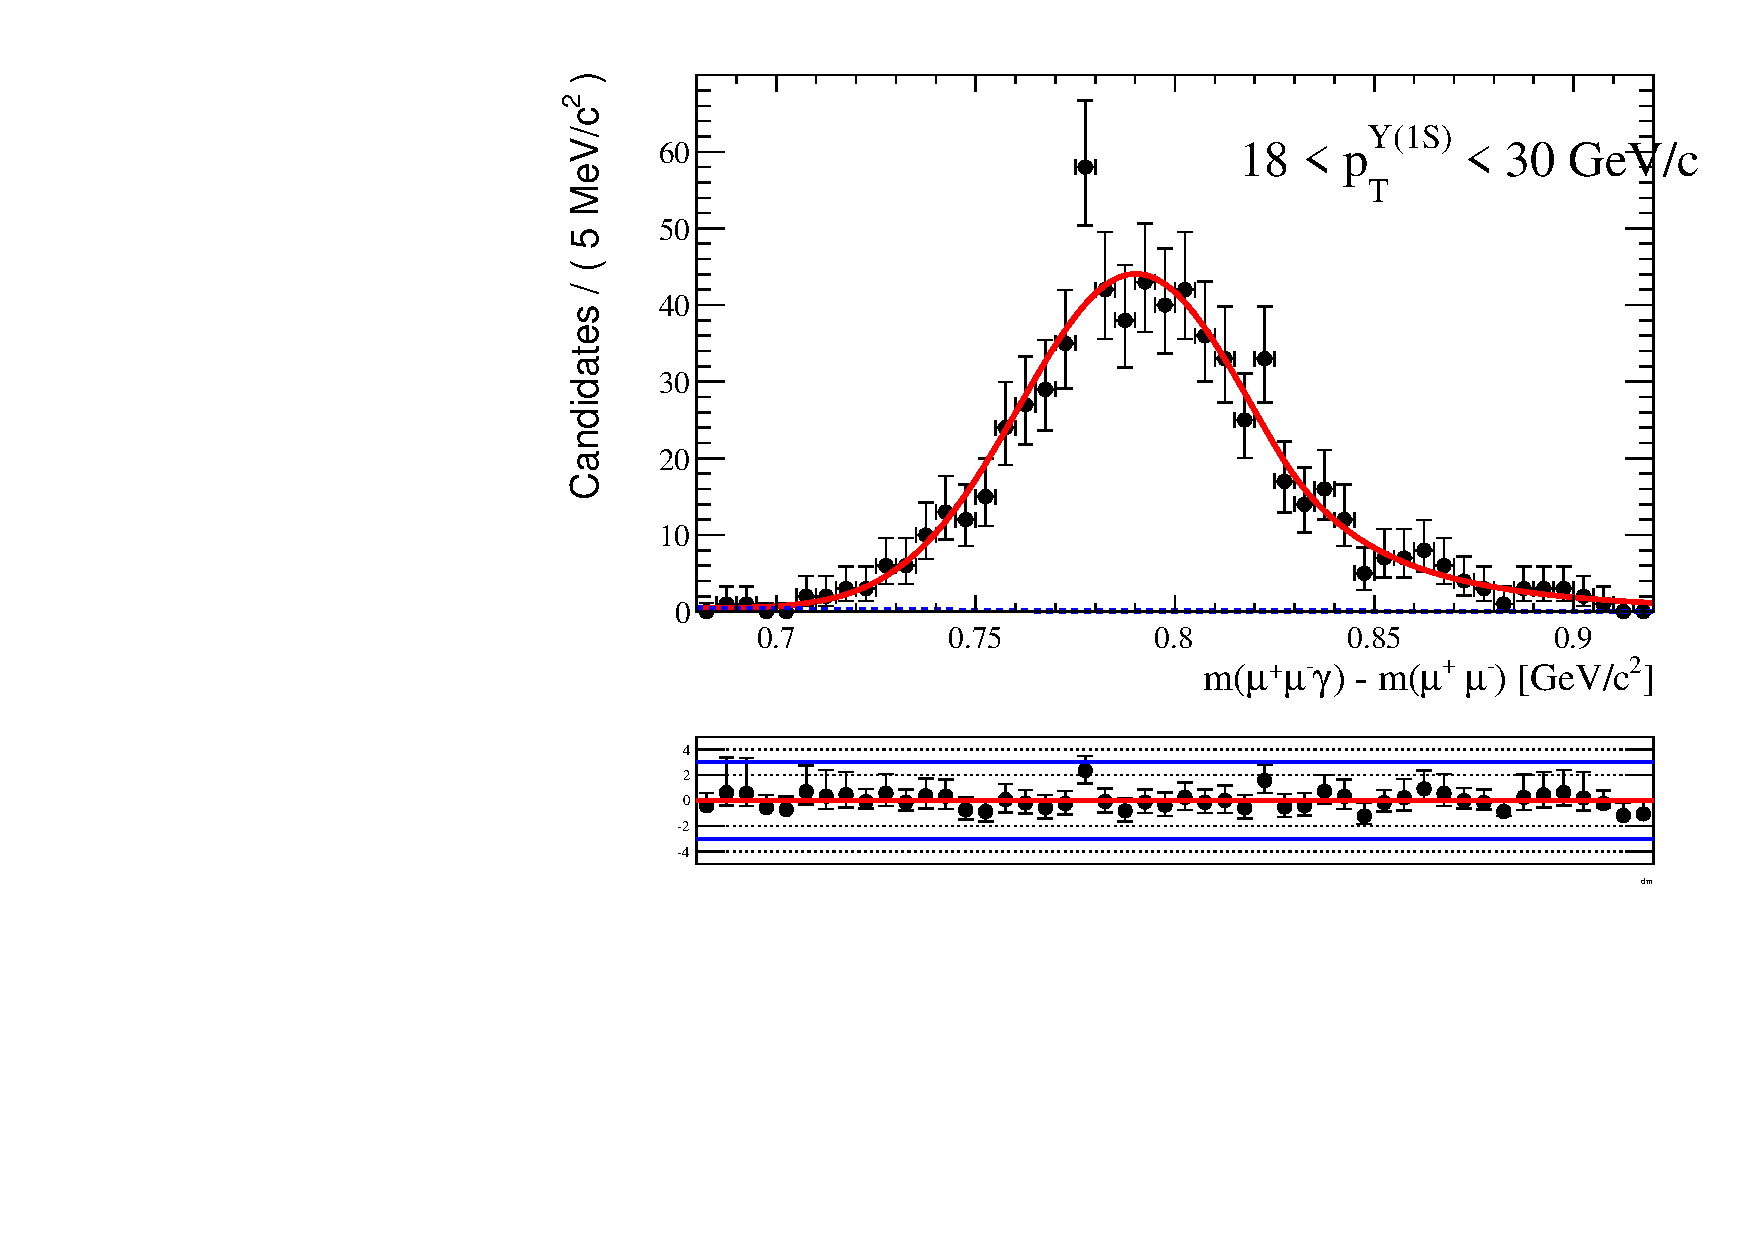
\includegraphics[width=0.16\linewidth]{fit_mc/chib12_18_30}
      \caption{\chiboneTwoP}
      \label{fig:fit_mc_chiboneTwoP}
    \end{subfigure}
    \begin{subfigure}[b]{\textwidth}
      \centering
      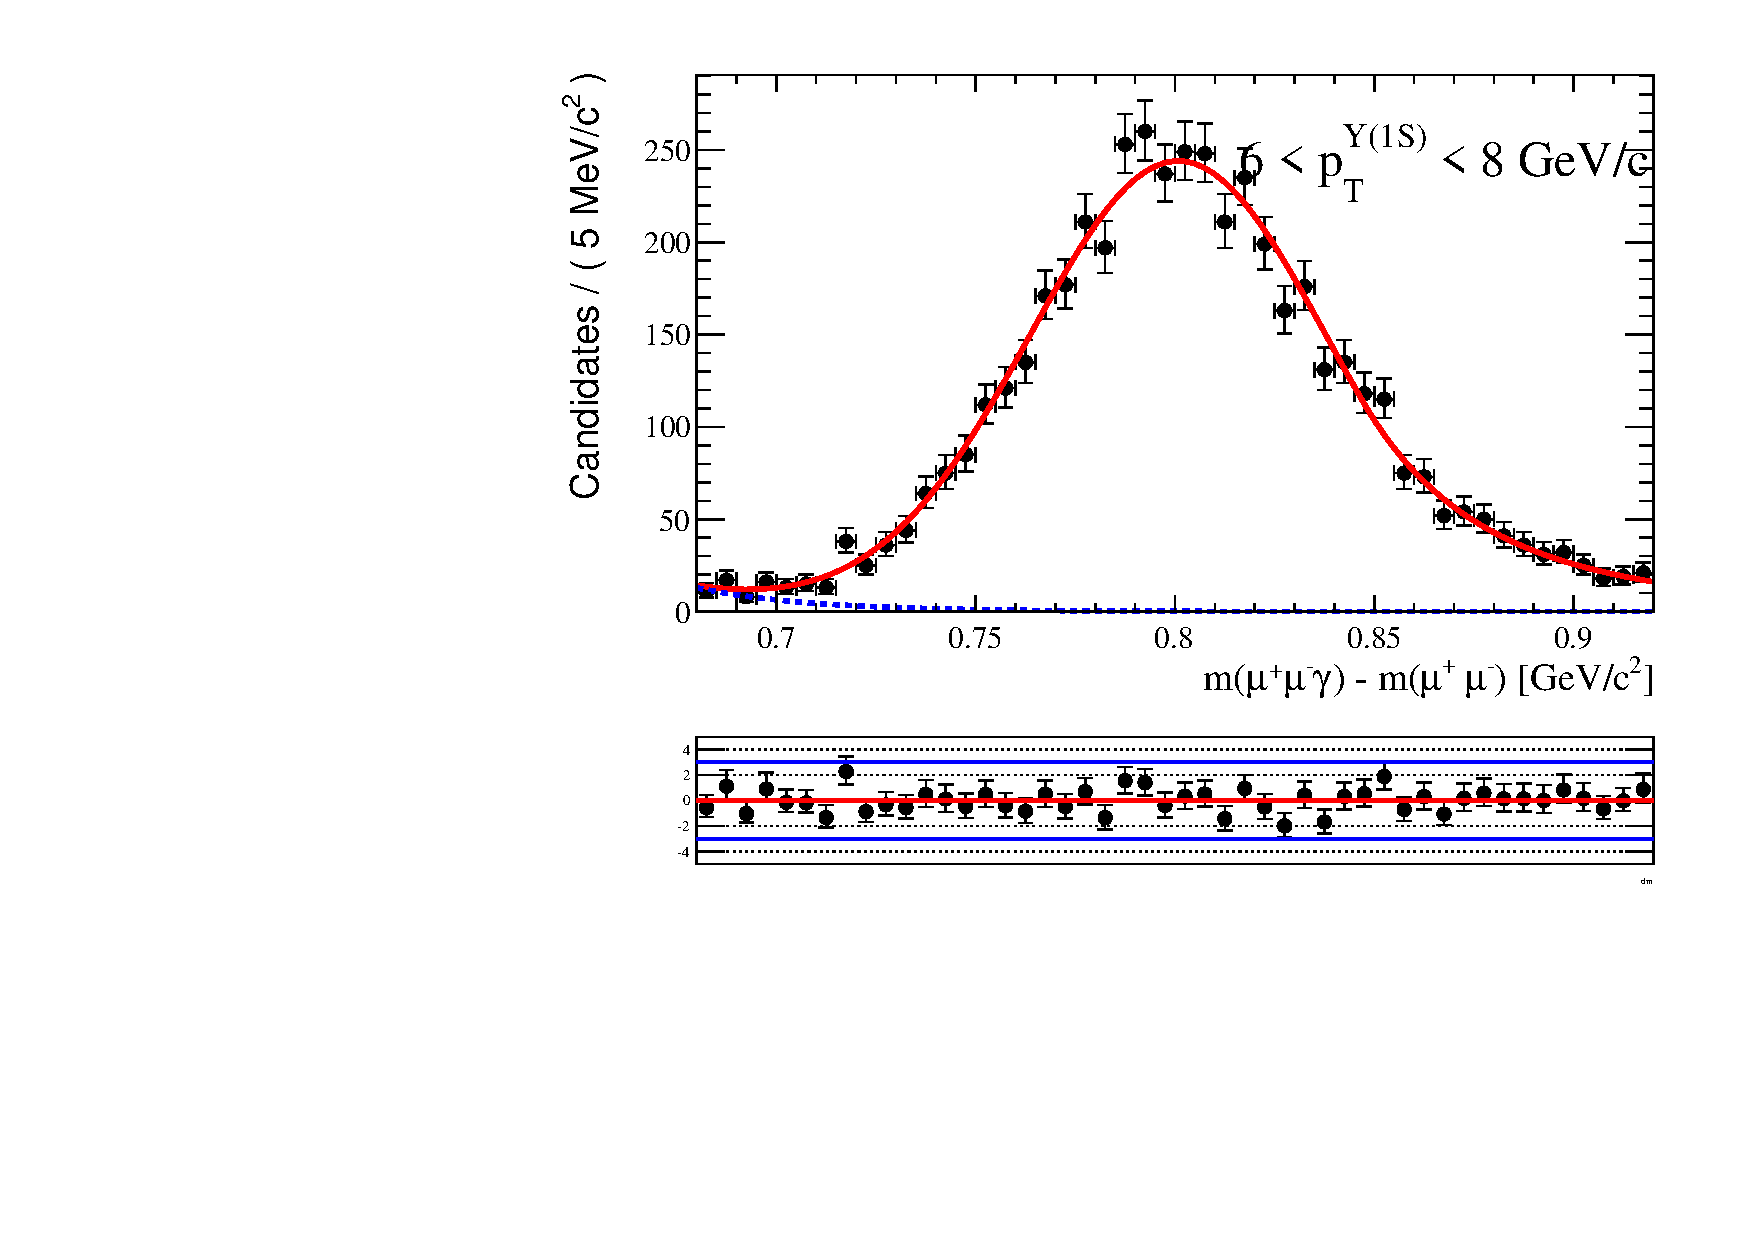
\includegraphics[width=0.16\linewidth]{fit_mc/chib22_6_8}
      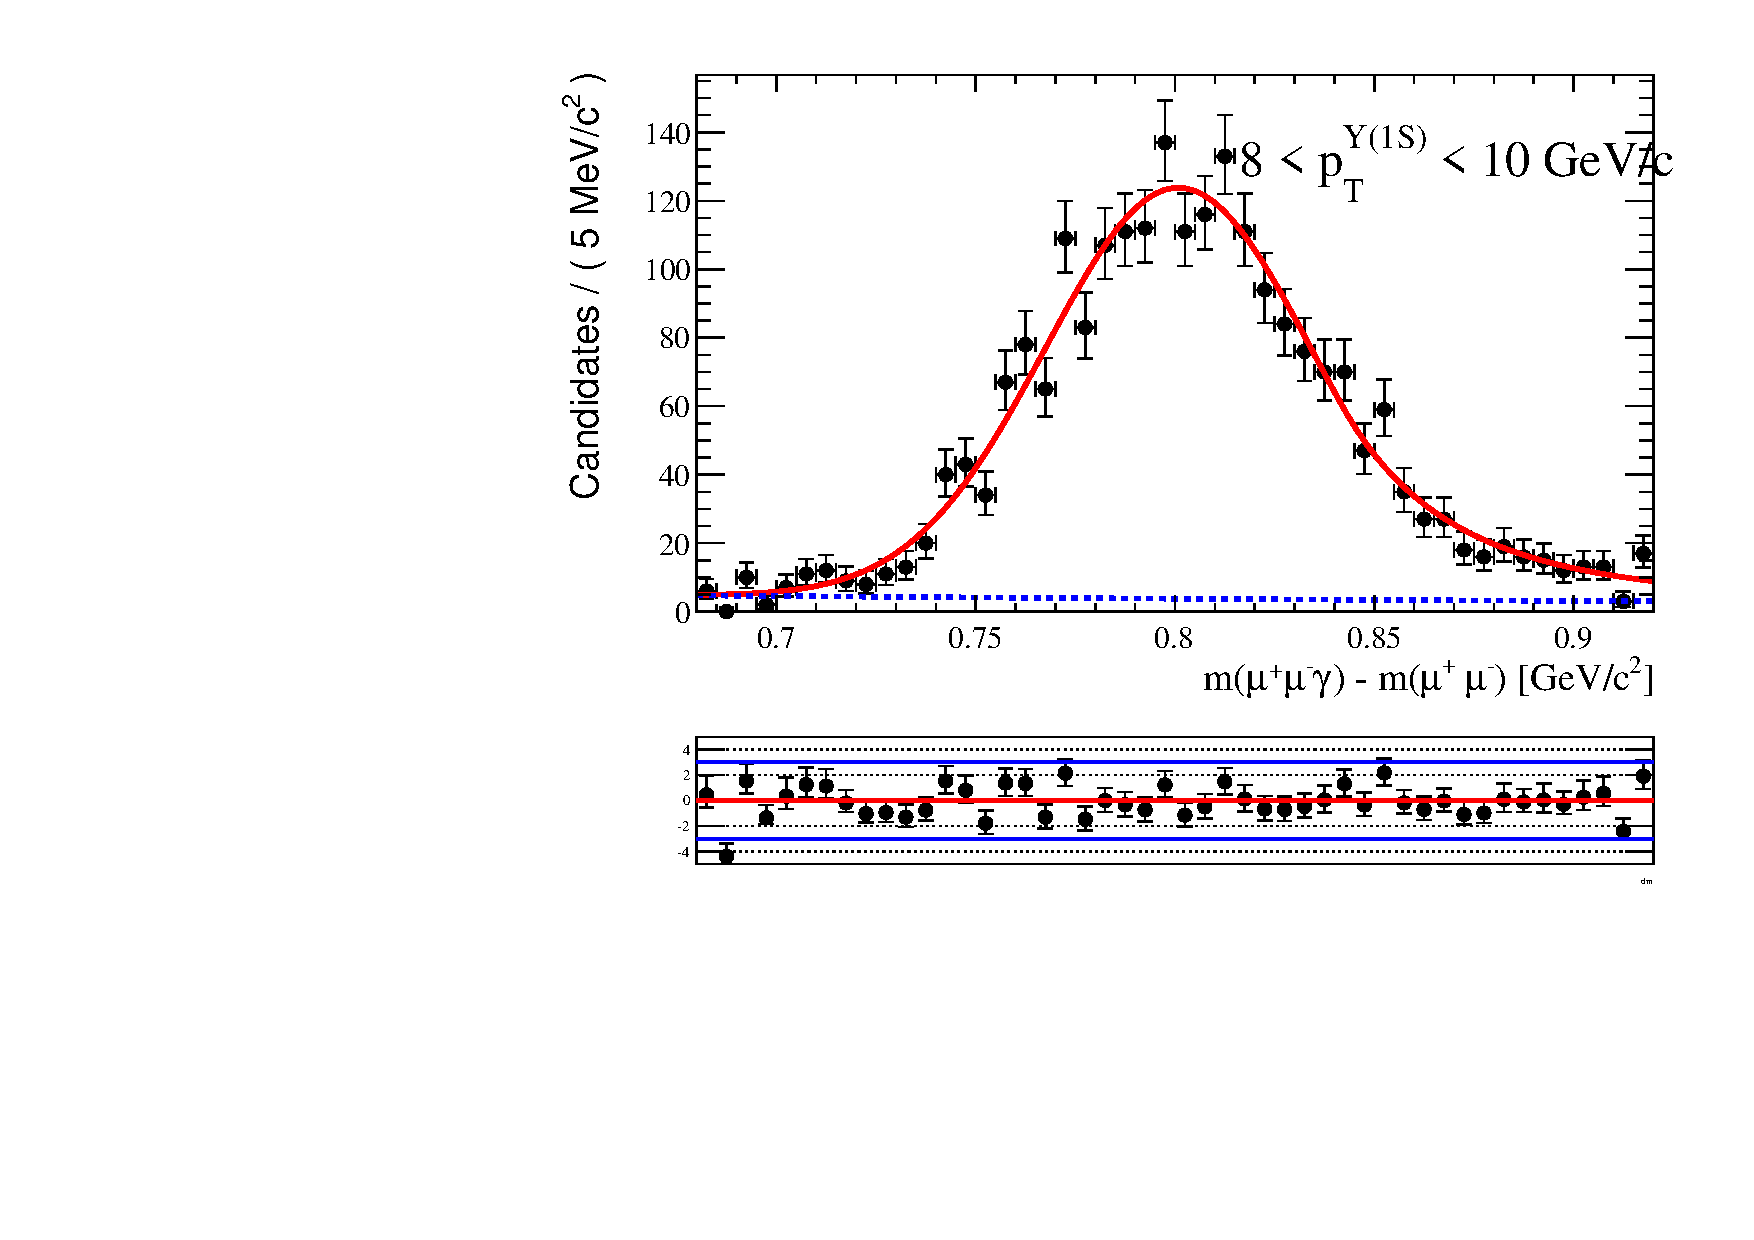
\includegraphics[width=0.16\linewidth]{fit_mc/chib22_8_10}
      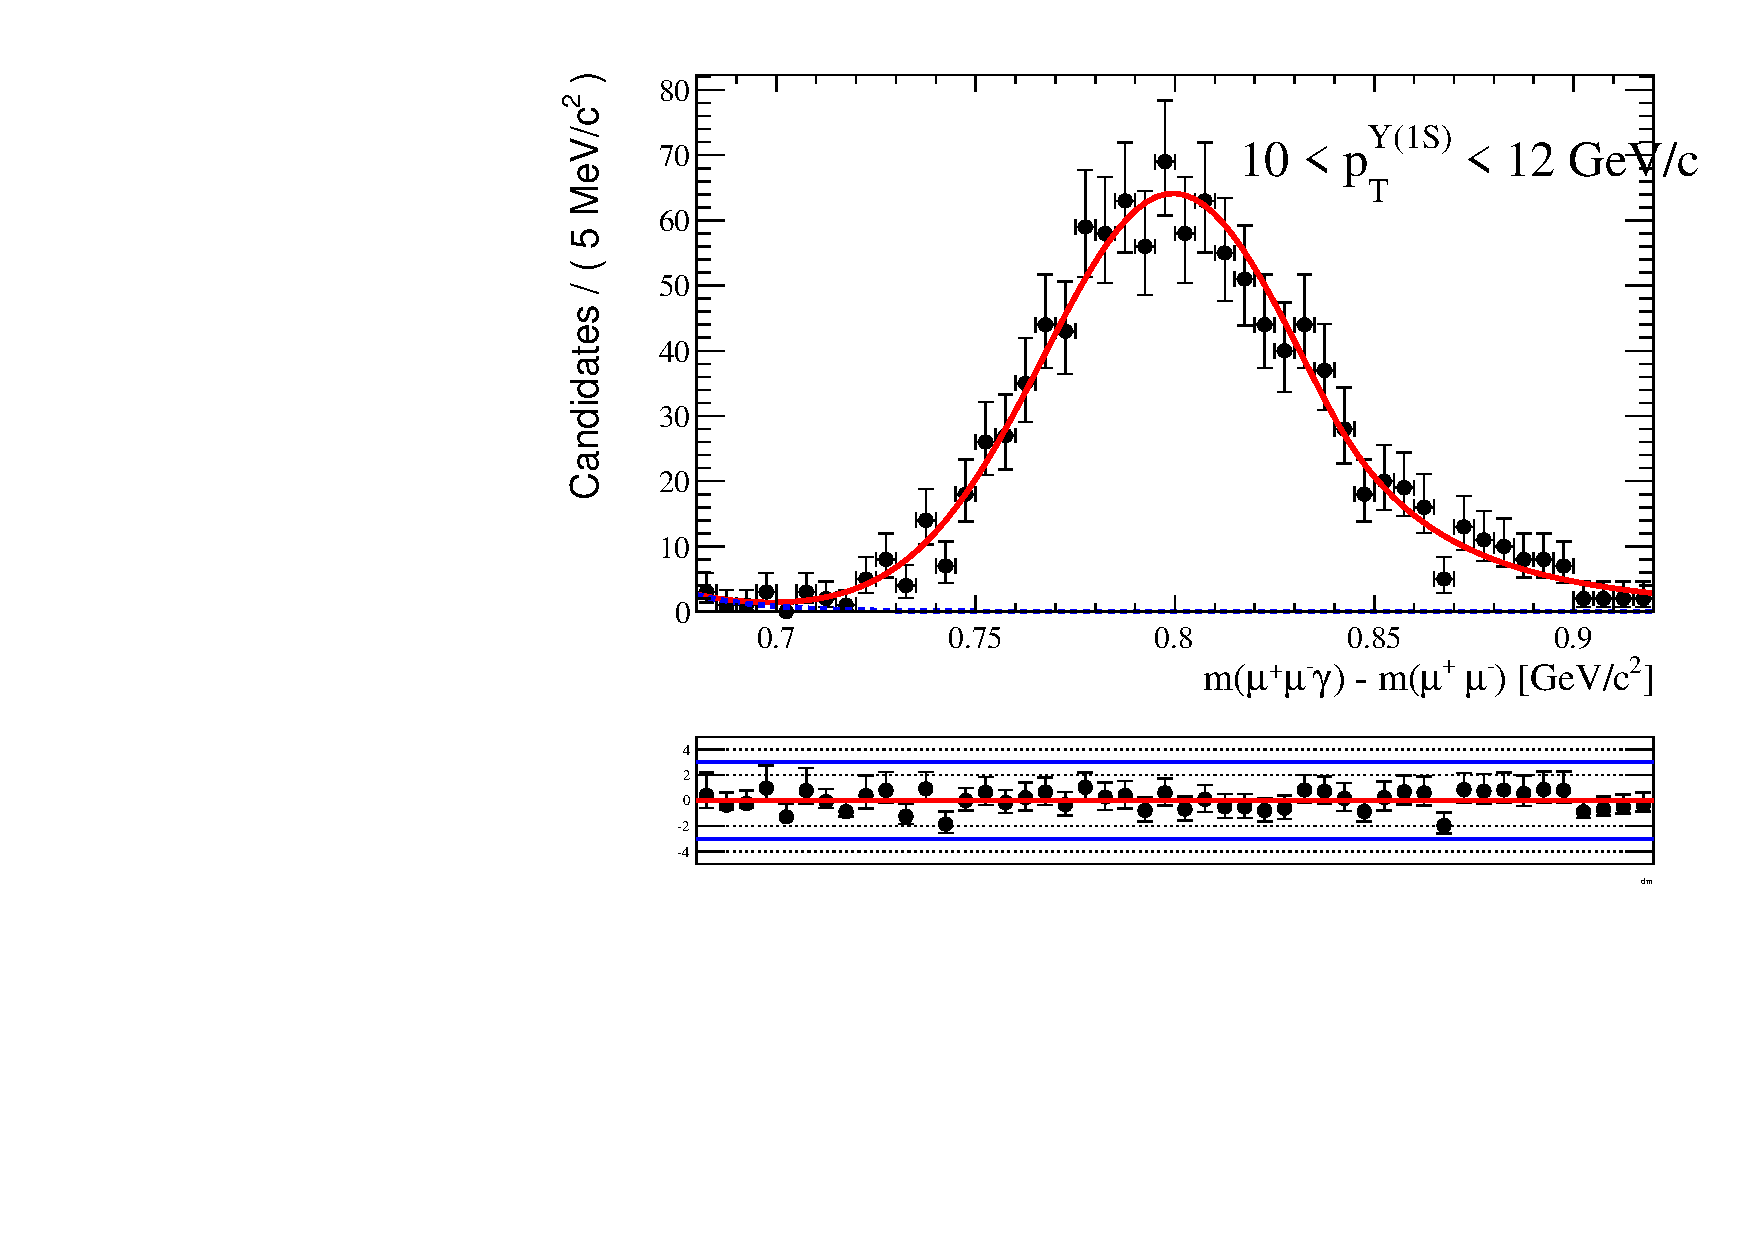
\includegraphics[width=0.16\linewidth]{fit_mc/chib22_10_12}
      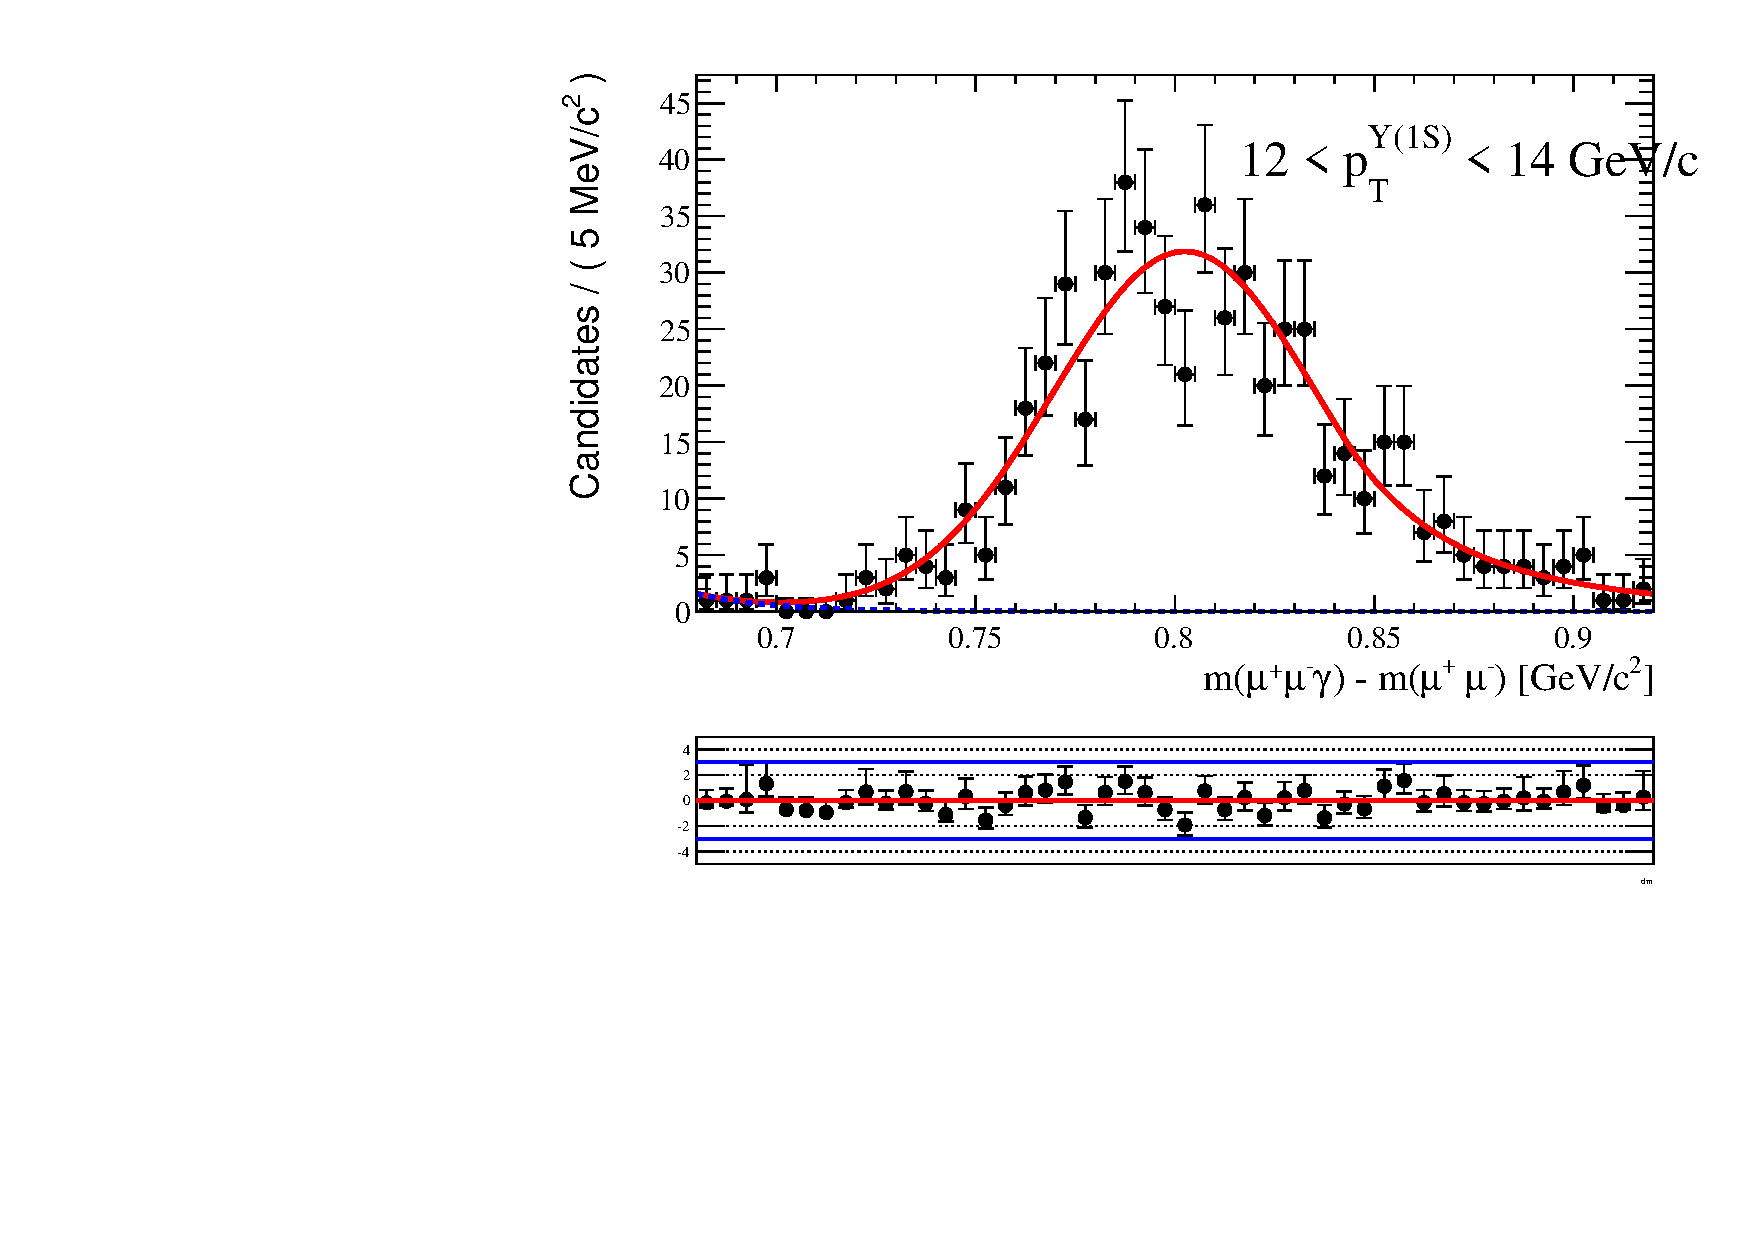
\includegraphics[width=0.16\linewidth]{fit_mc/chib22_12_14}
      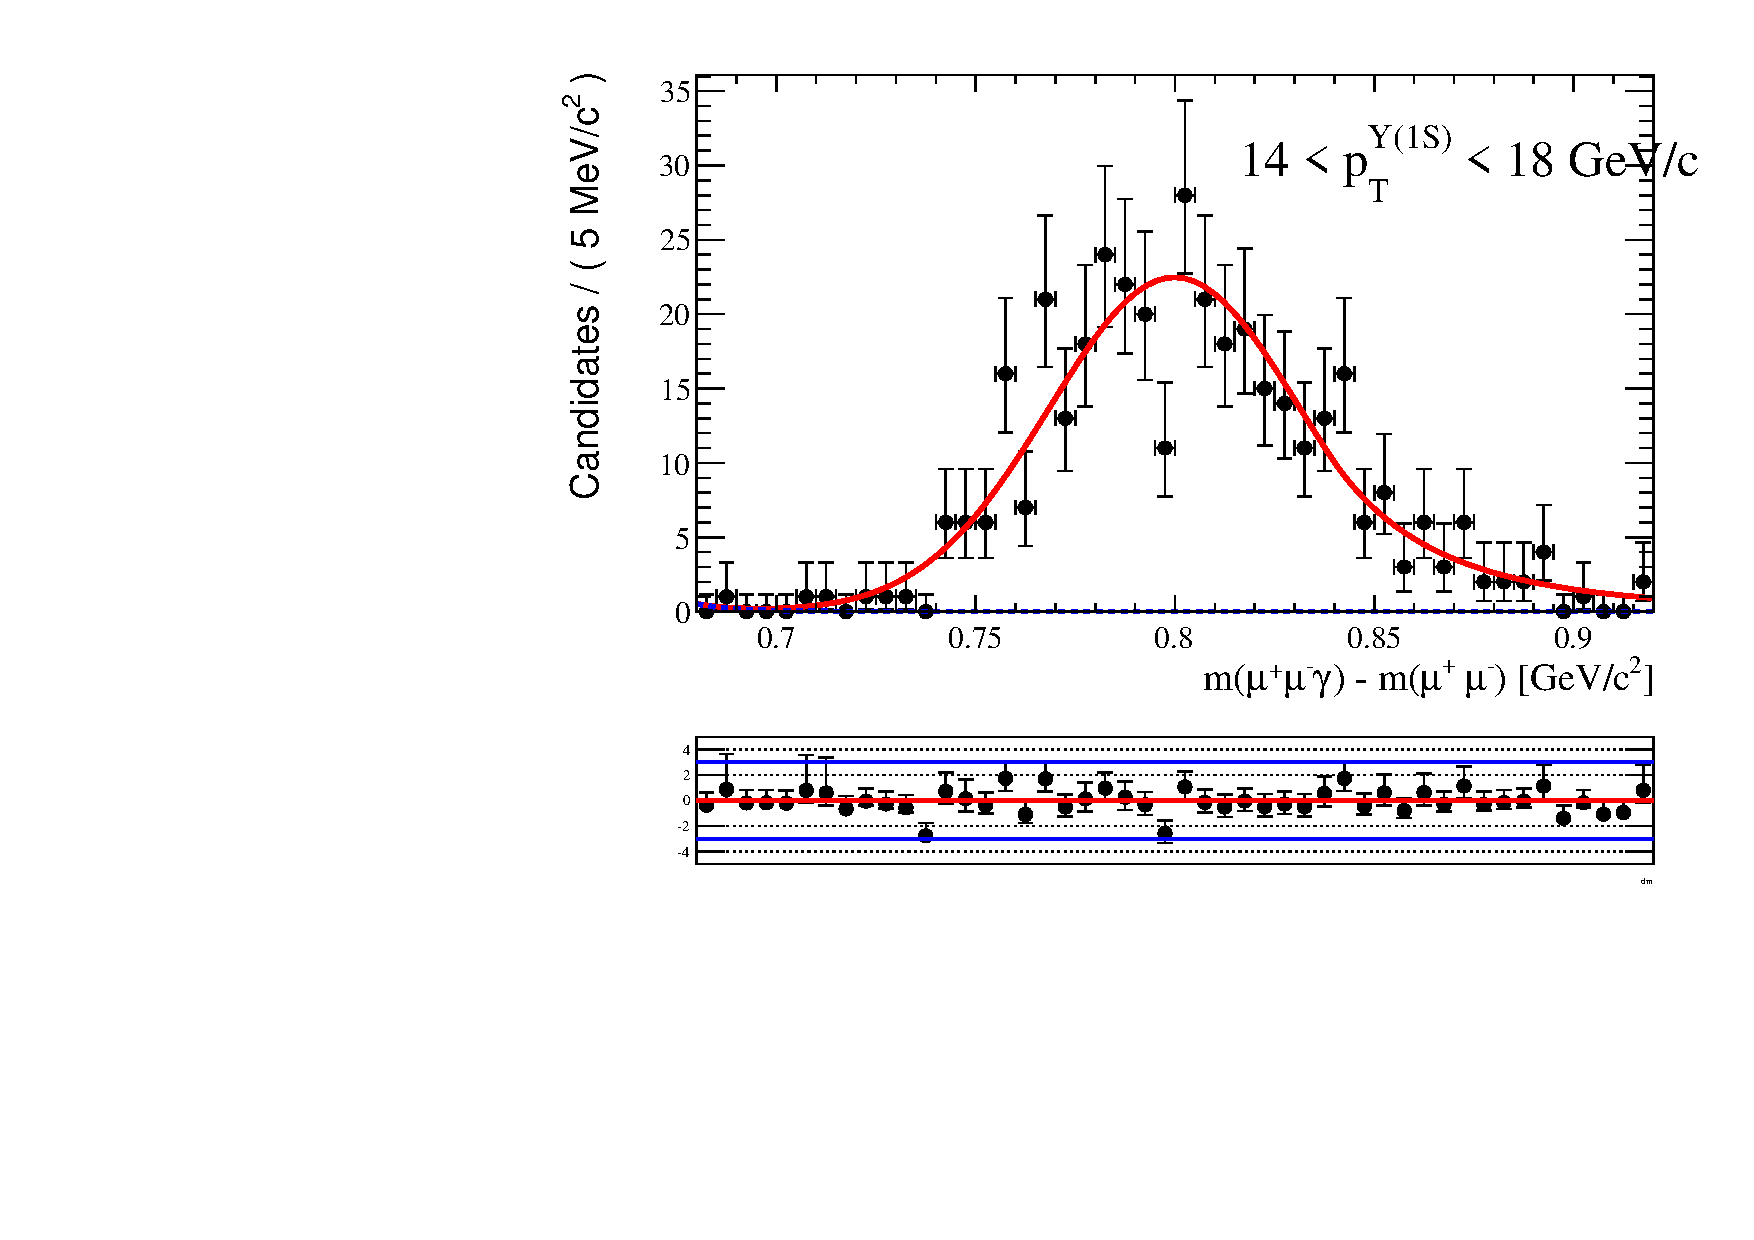
\includegraphics[width=0.16\linewidth]{fit_mc/chib22_14_18}
      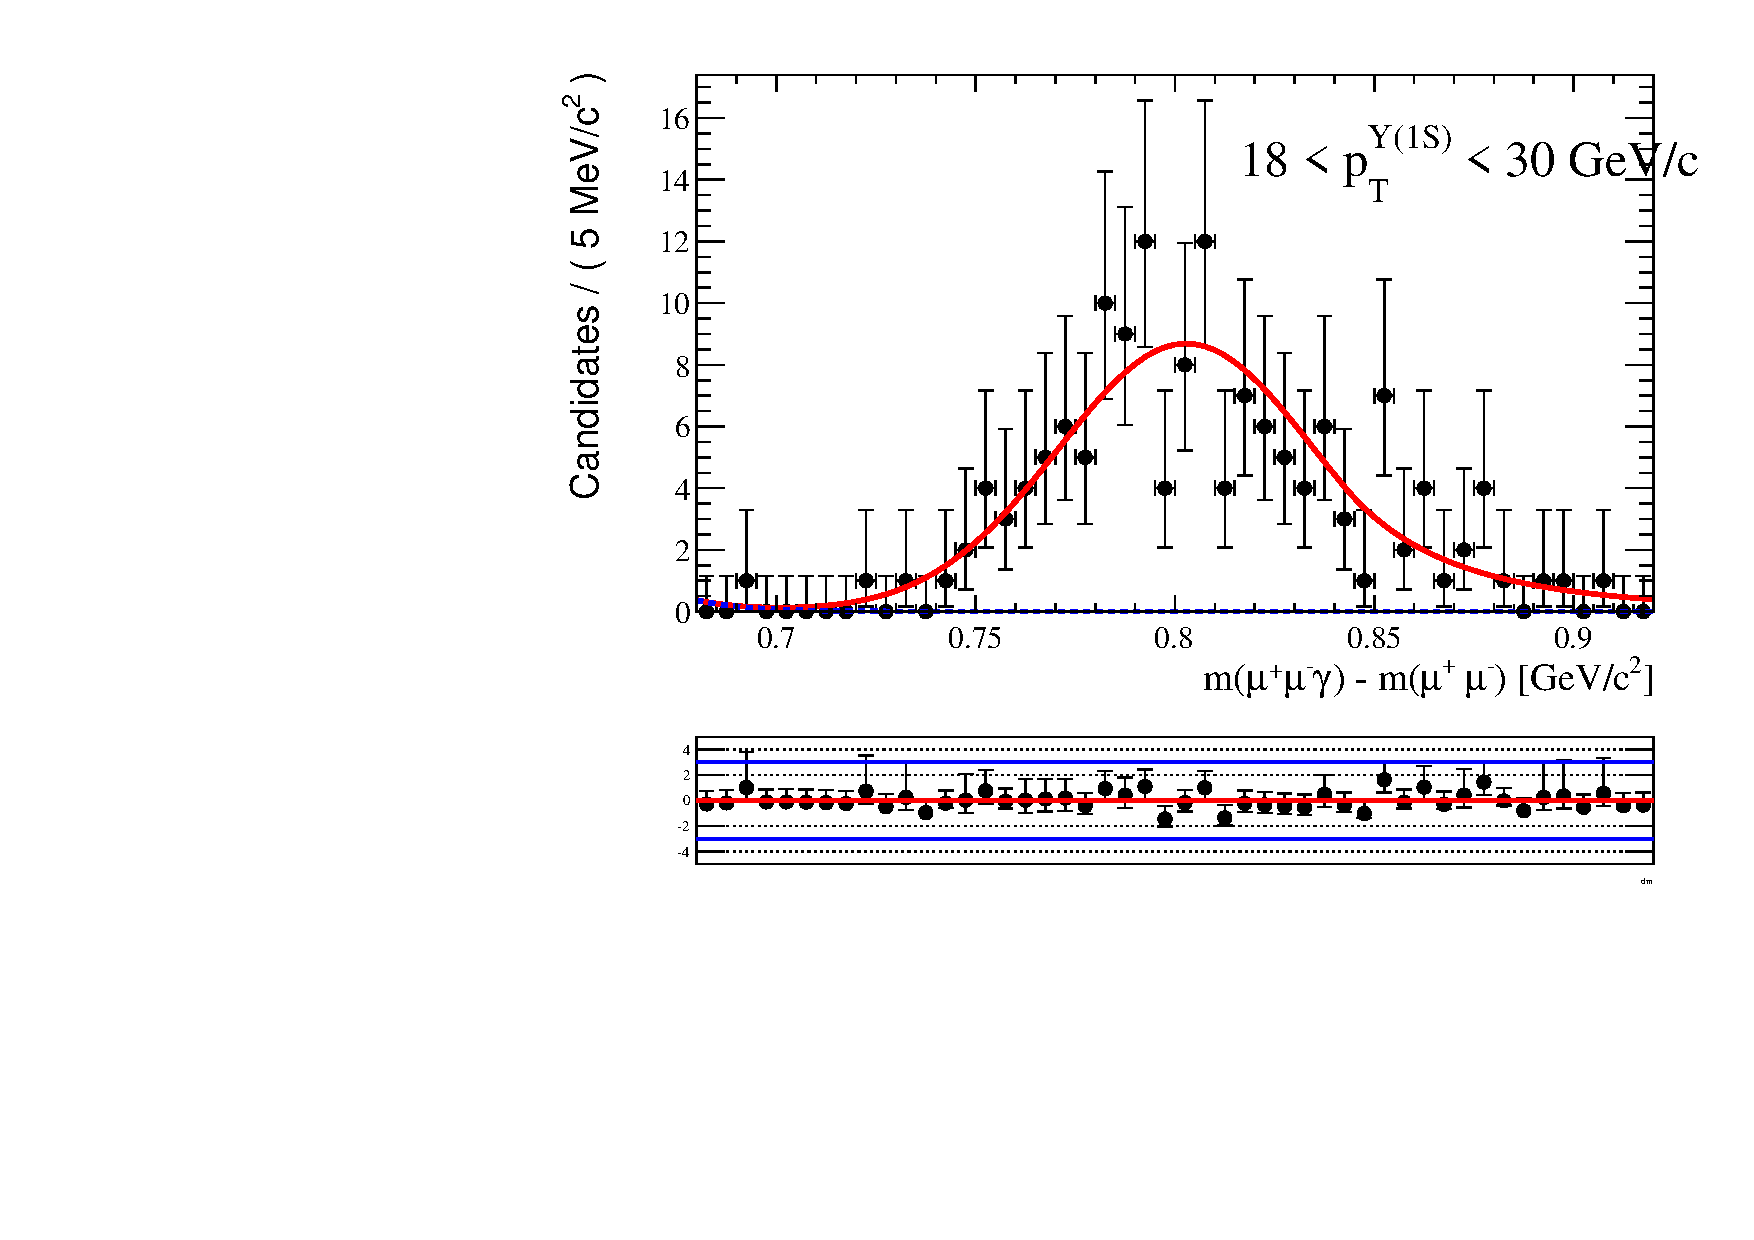
\includegraphics[width=0.16\linewidth]{fit_mc/chib22_18_30}
      \caption{\chibtwoTwoP}
      \label{fig:fit_mc_chibtwoTwoP}
    \end{subfigure}    
    \begin{subfigure}[b]{\textwidth}
      \centering
      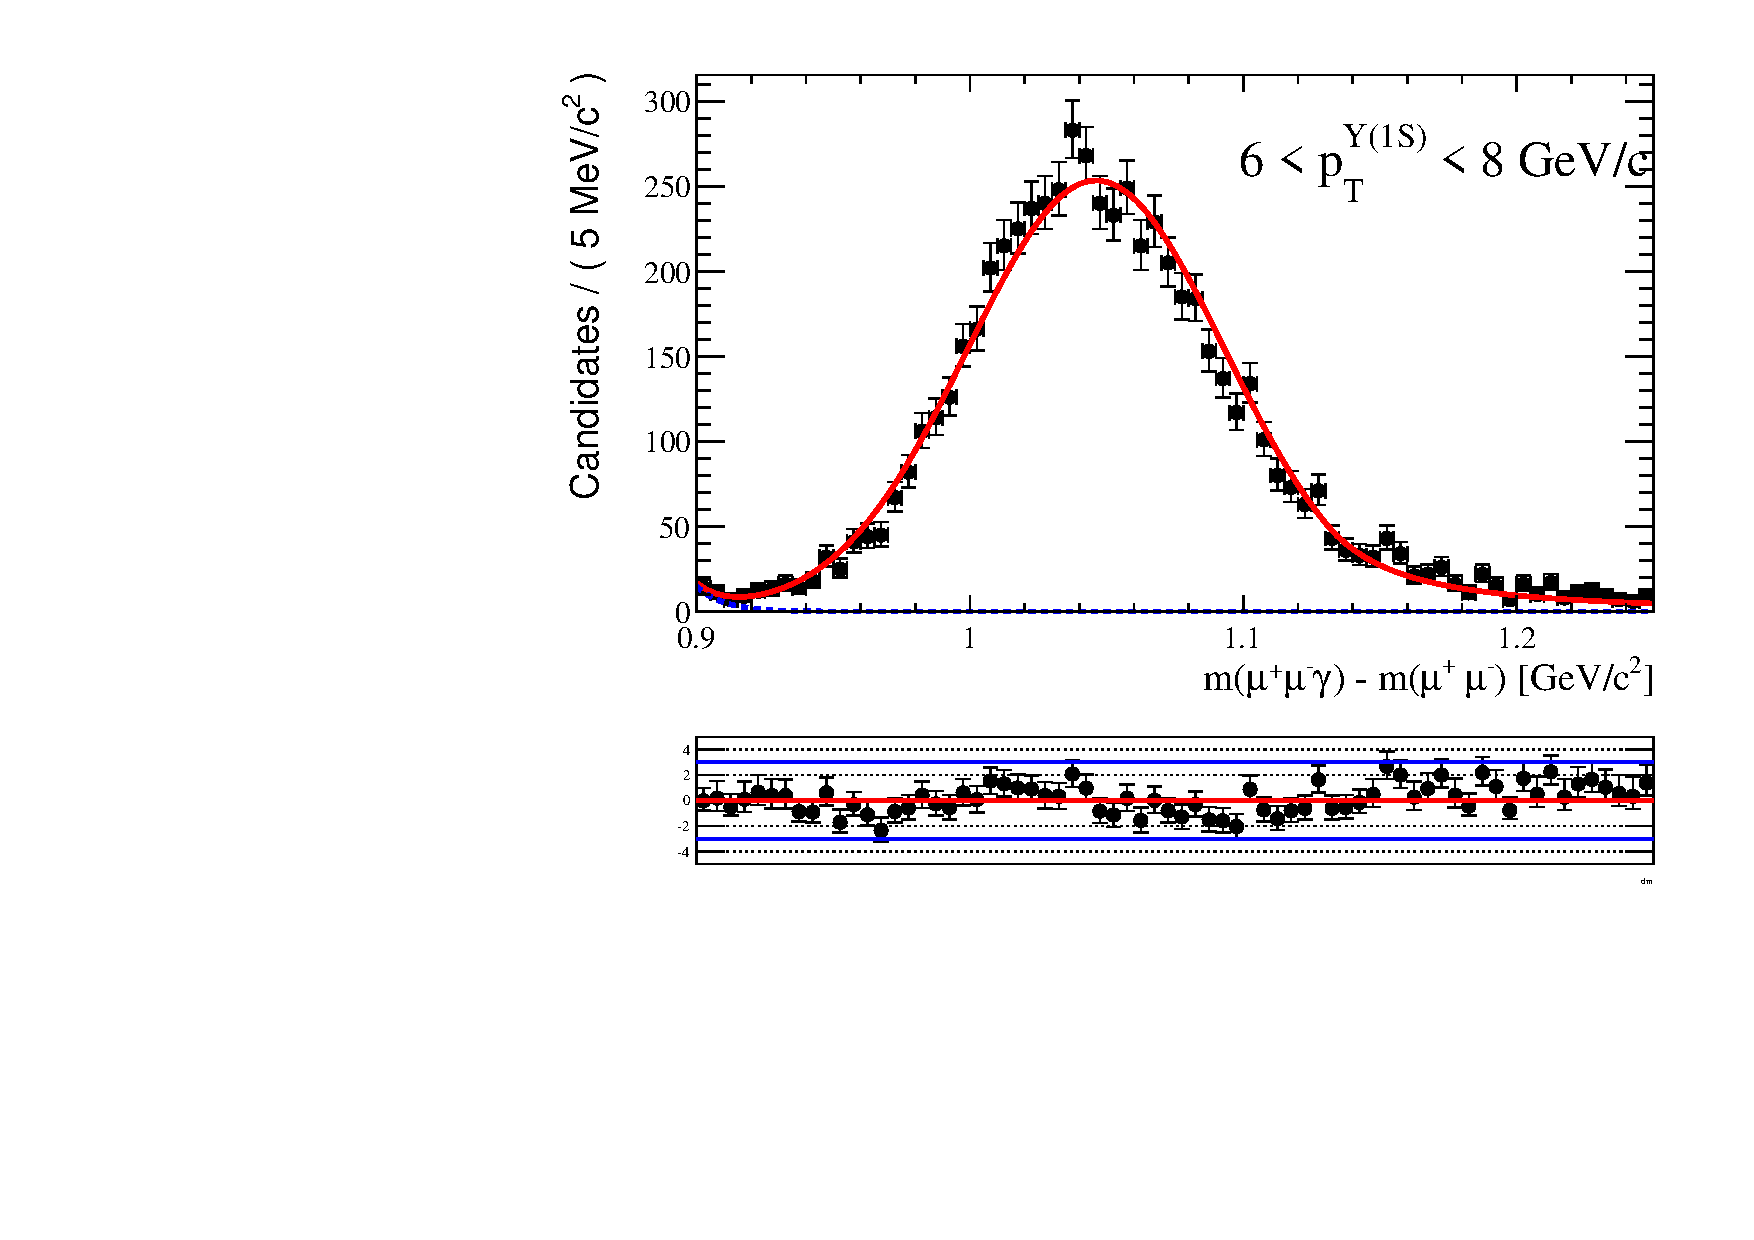
\includegraphics[width=0.16\linewidth]{fit_mc/chib13_6_8}
      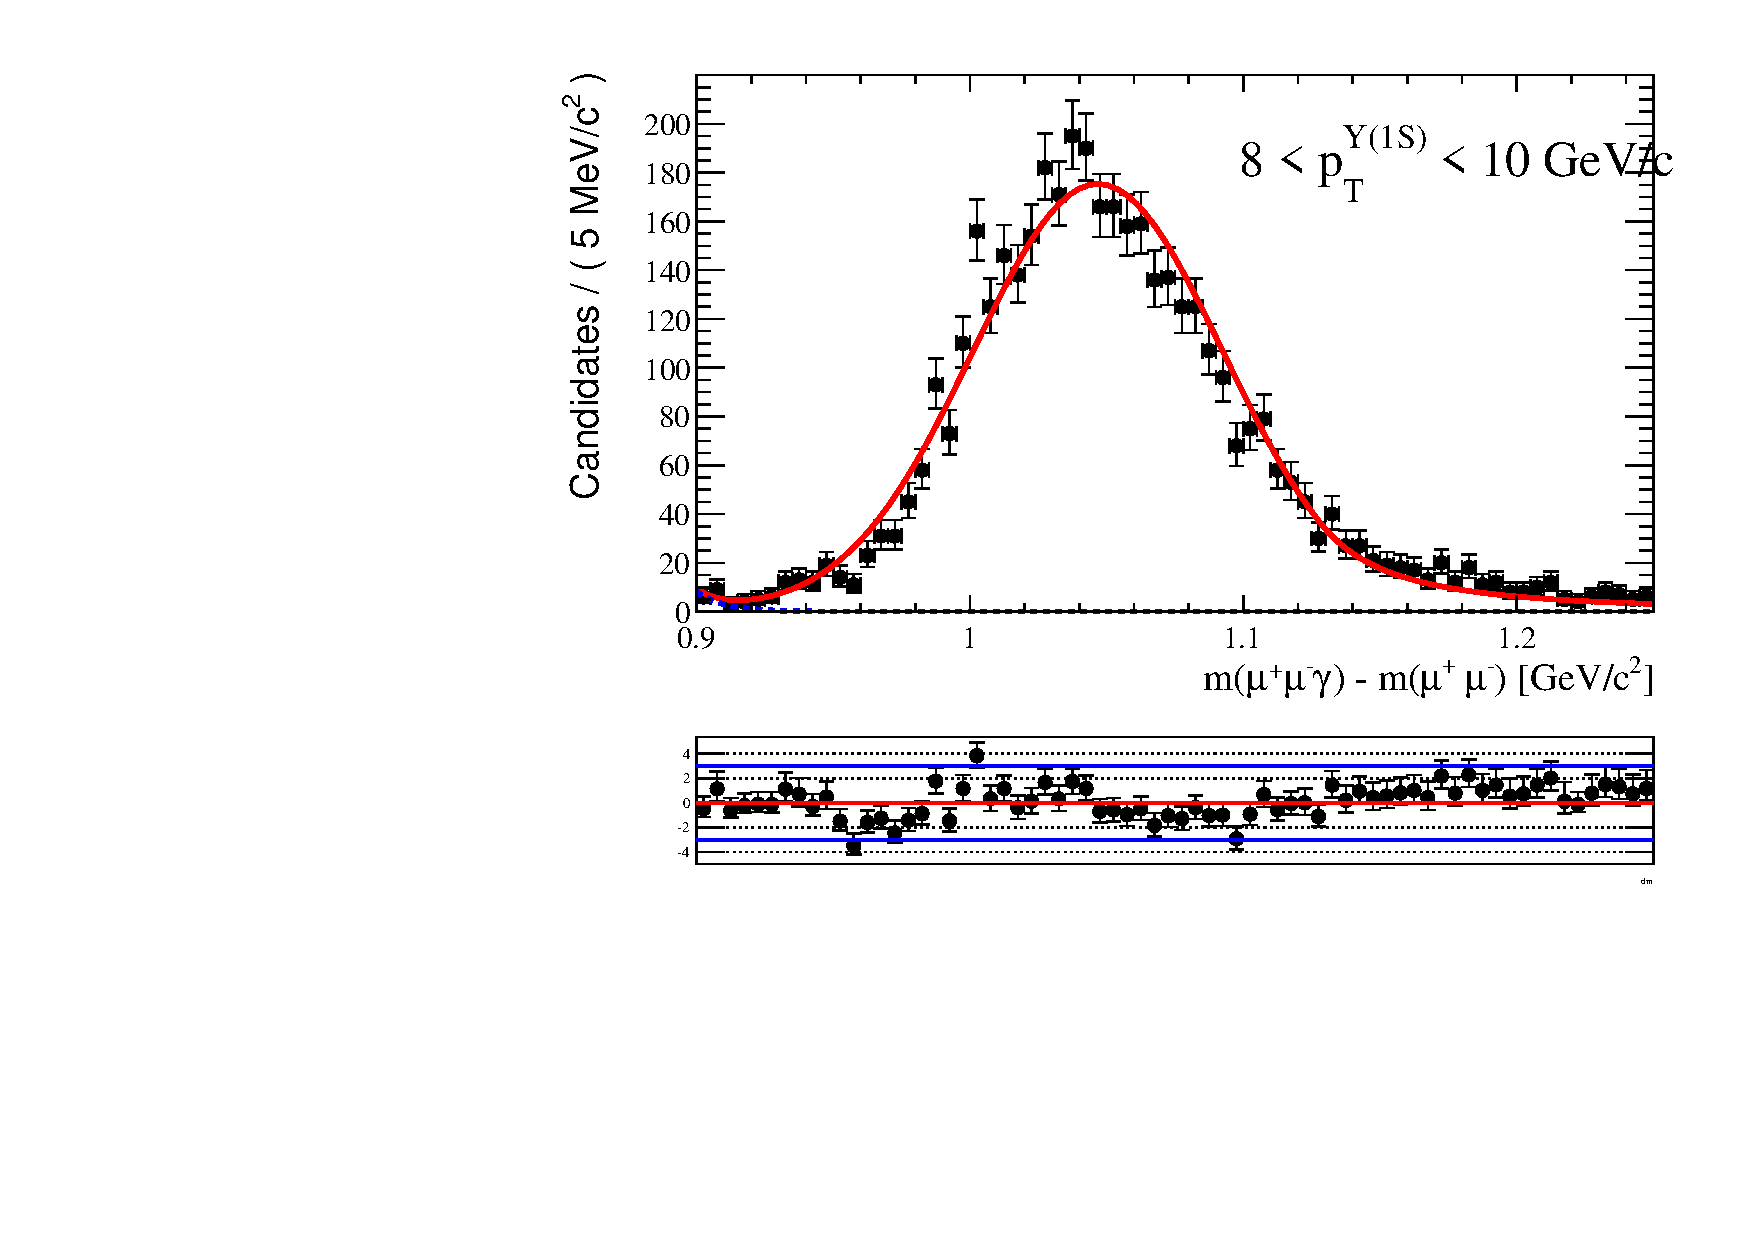
\includegraphics[width=0.16\linewidth]{fit_mc/chib13_8_10}
      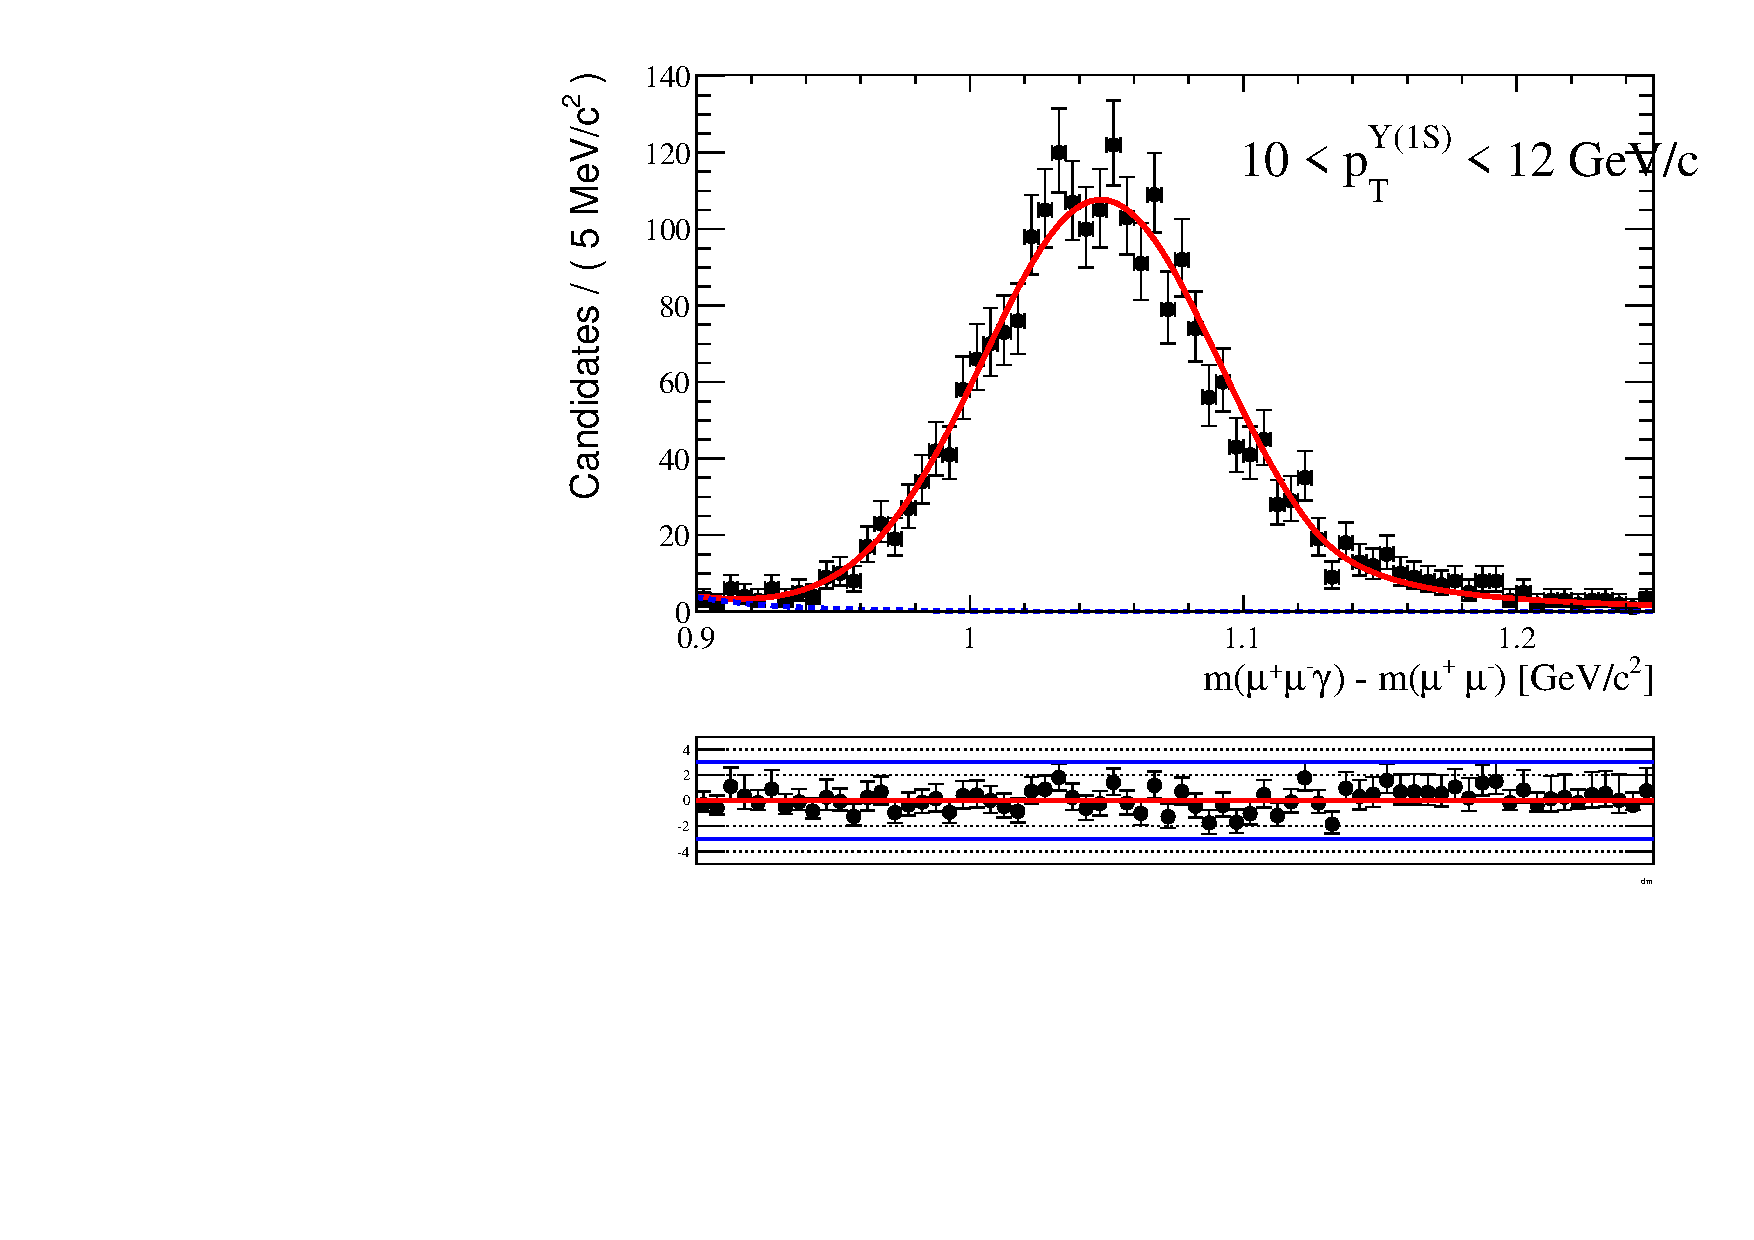
\includegraphics[width=0.16\linewidth]{fit_mc/chib13_10_12}
      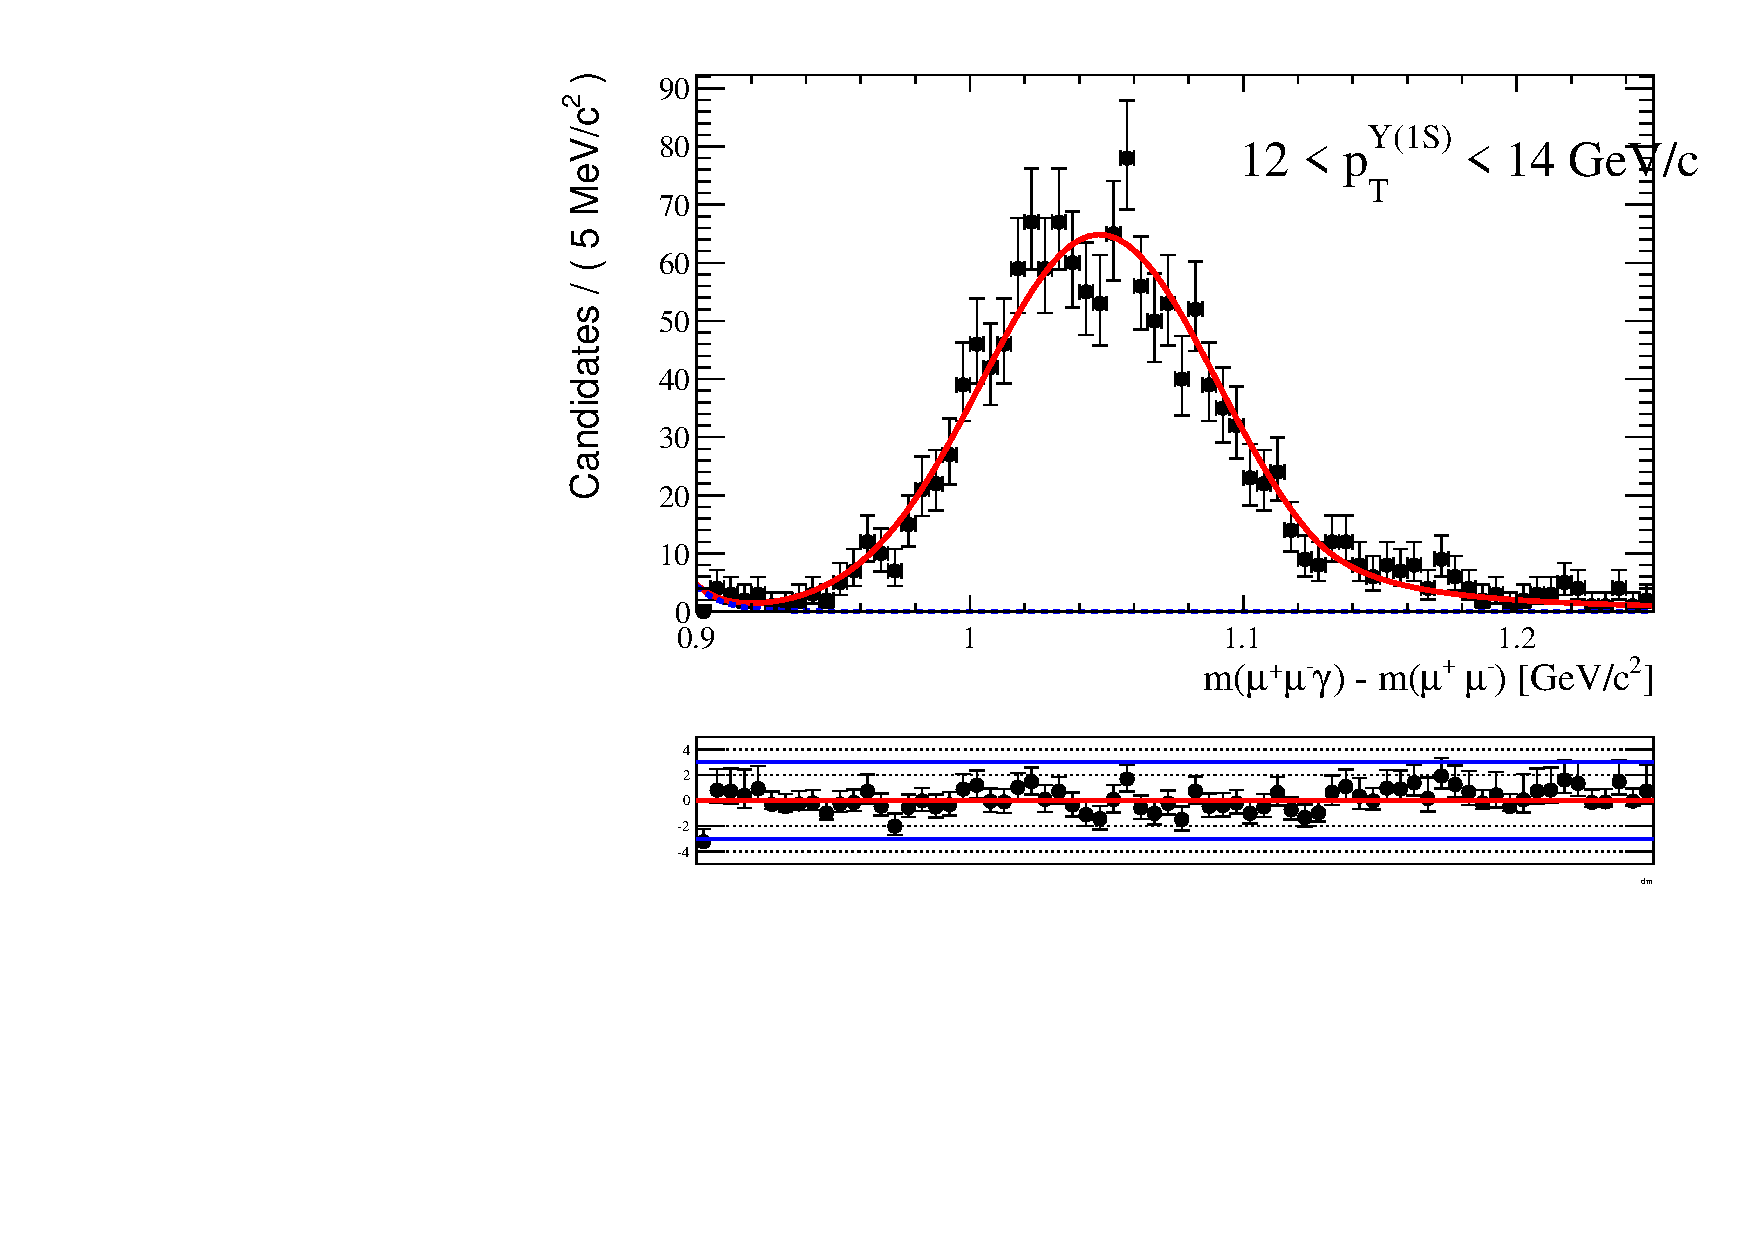
\includegraphics[width=0.16\linewidth]{fit_mc/chib13_12_14}
      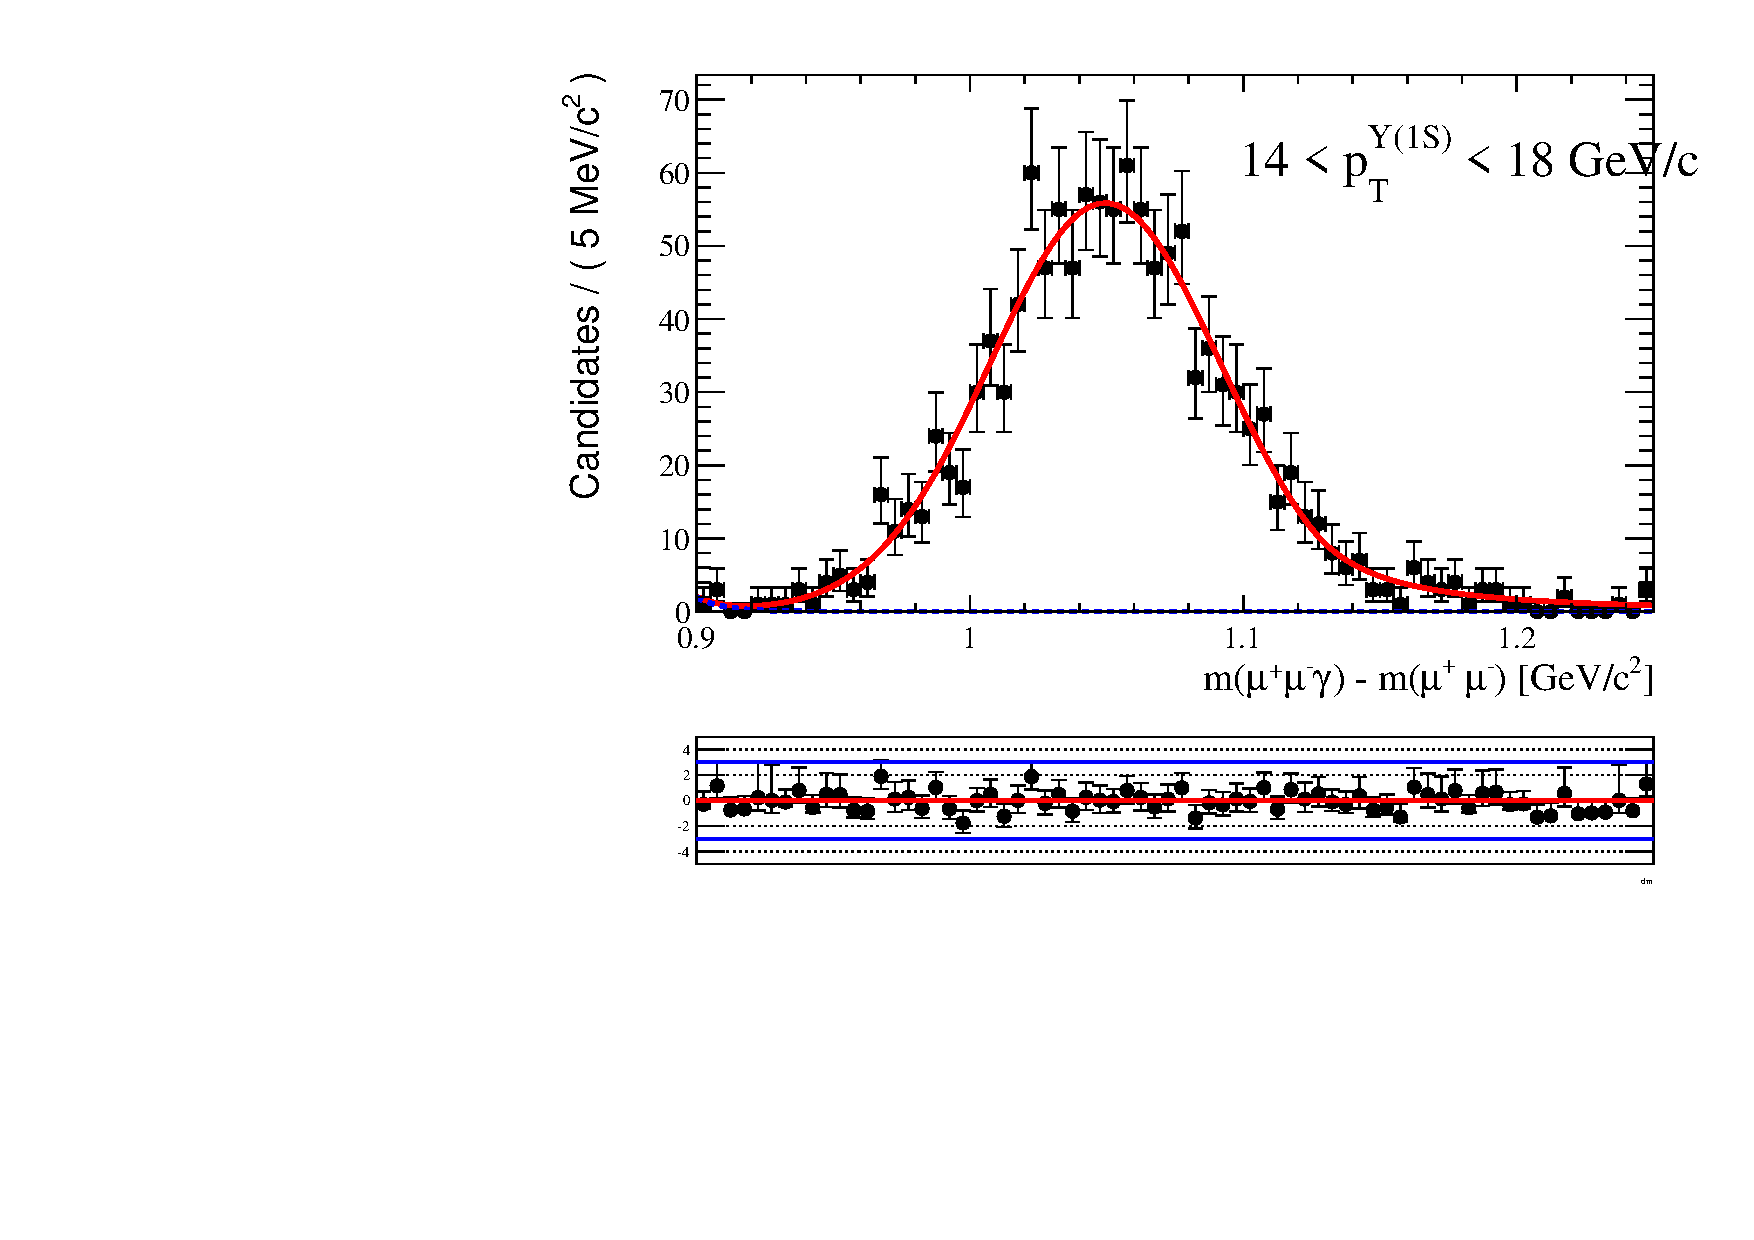
\includegraphics[width=0.16\linewidth]{fit_mc/chib13_14_18}
      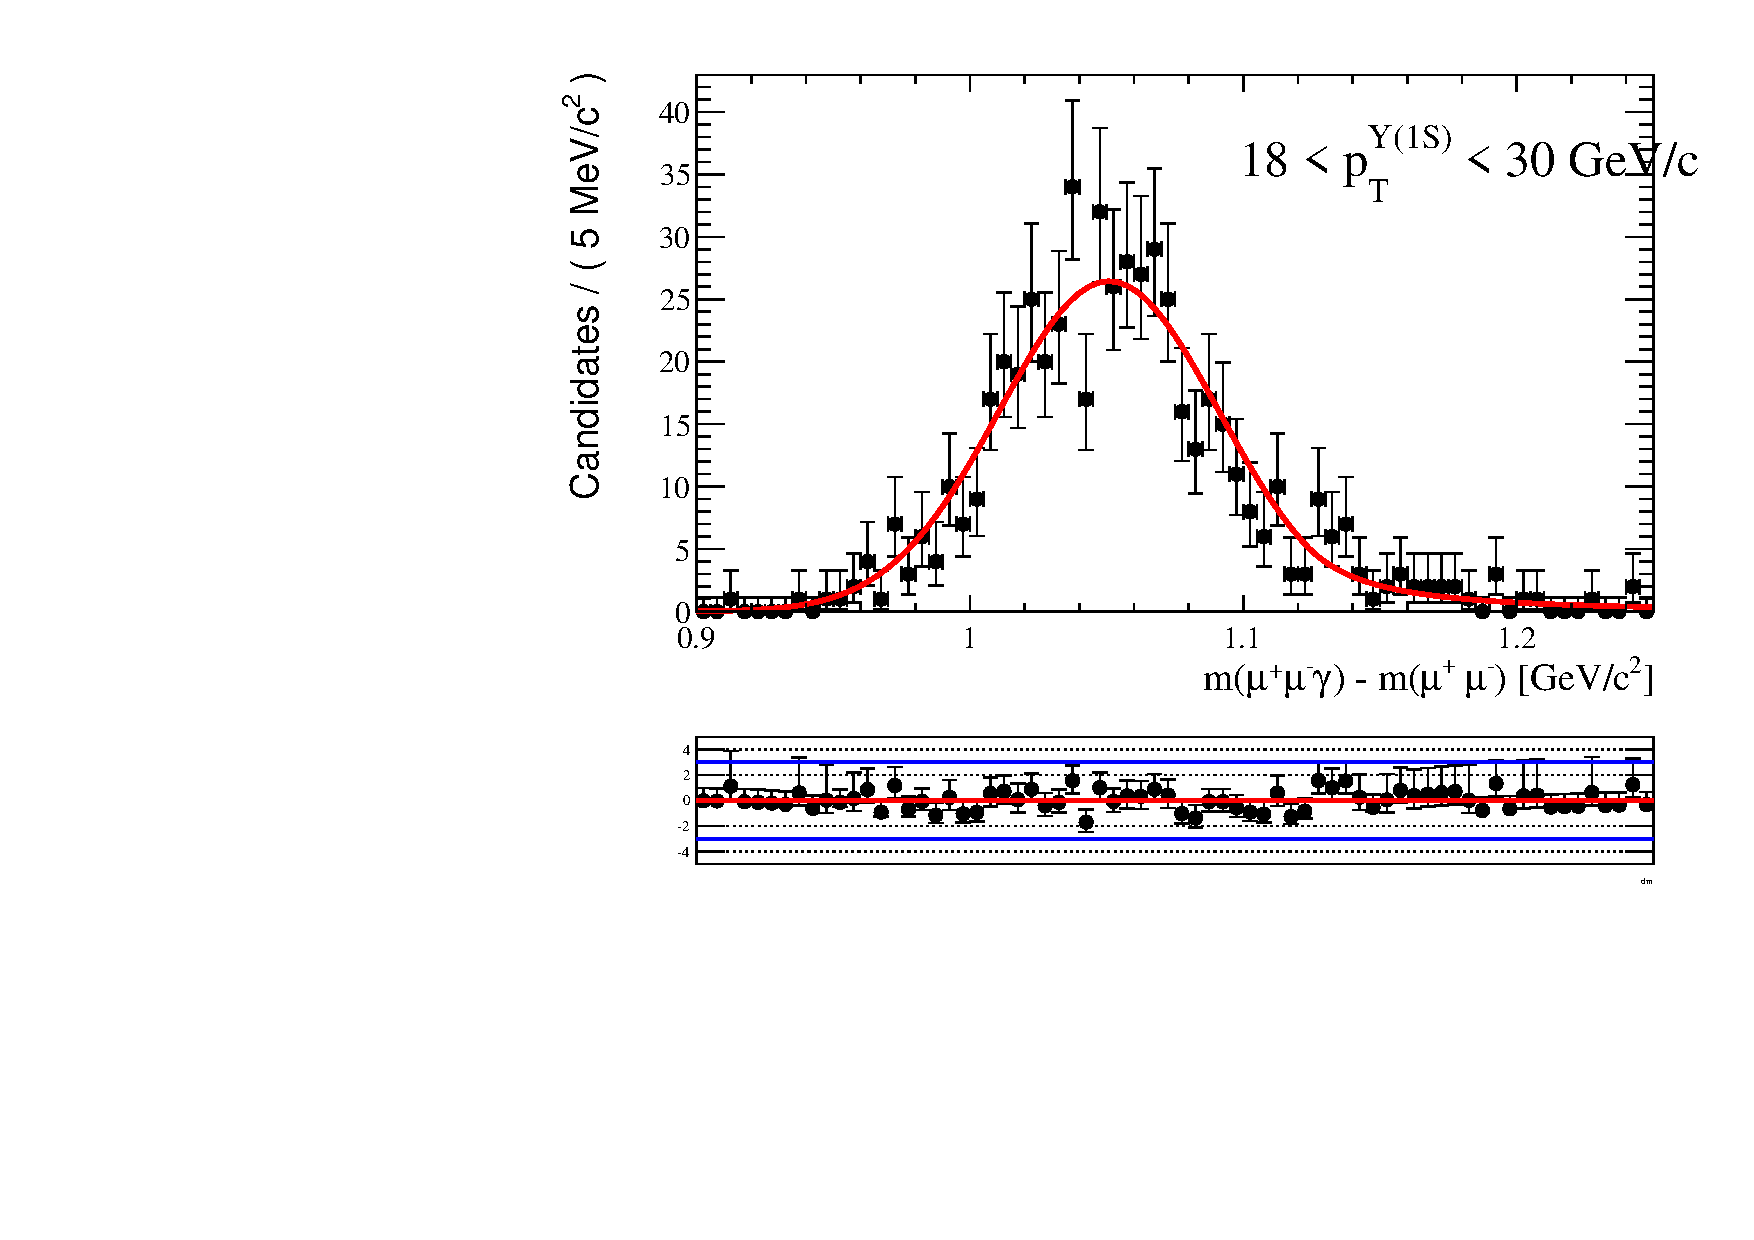
\includegraphics[width=0.16\linewidth]{fit_mc/chib13_18_30}
      \caption{\chiboneThreeP}
      \label{fig:fit_mc_chiboneThreeP}
    \end{subfigure}
    \begin{subfigure}[b]{\textwidth}
      \centering
      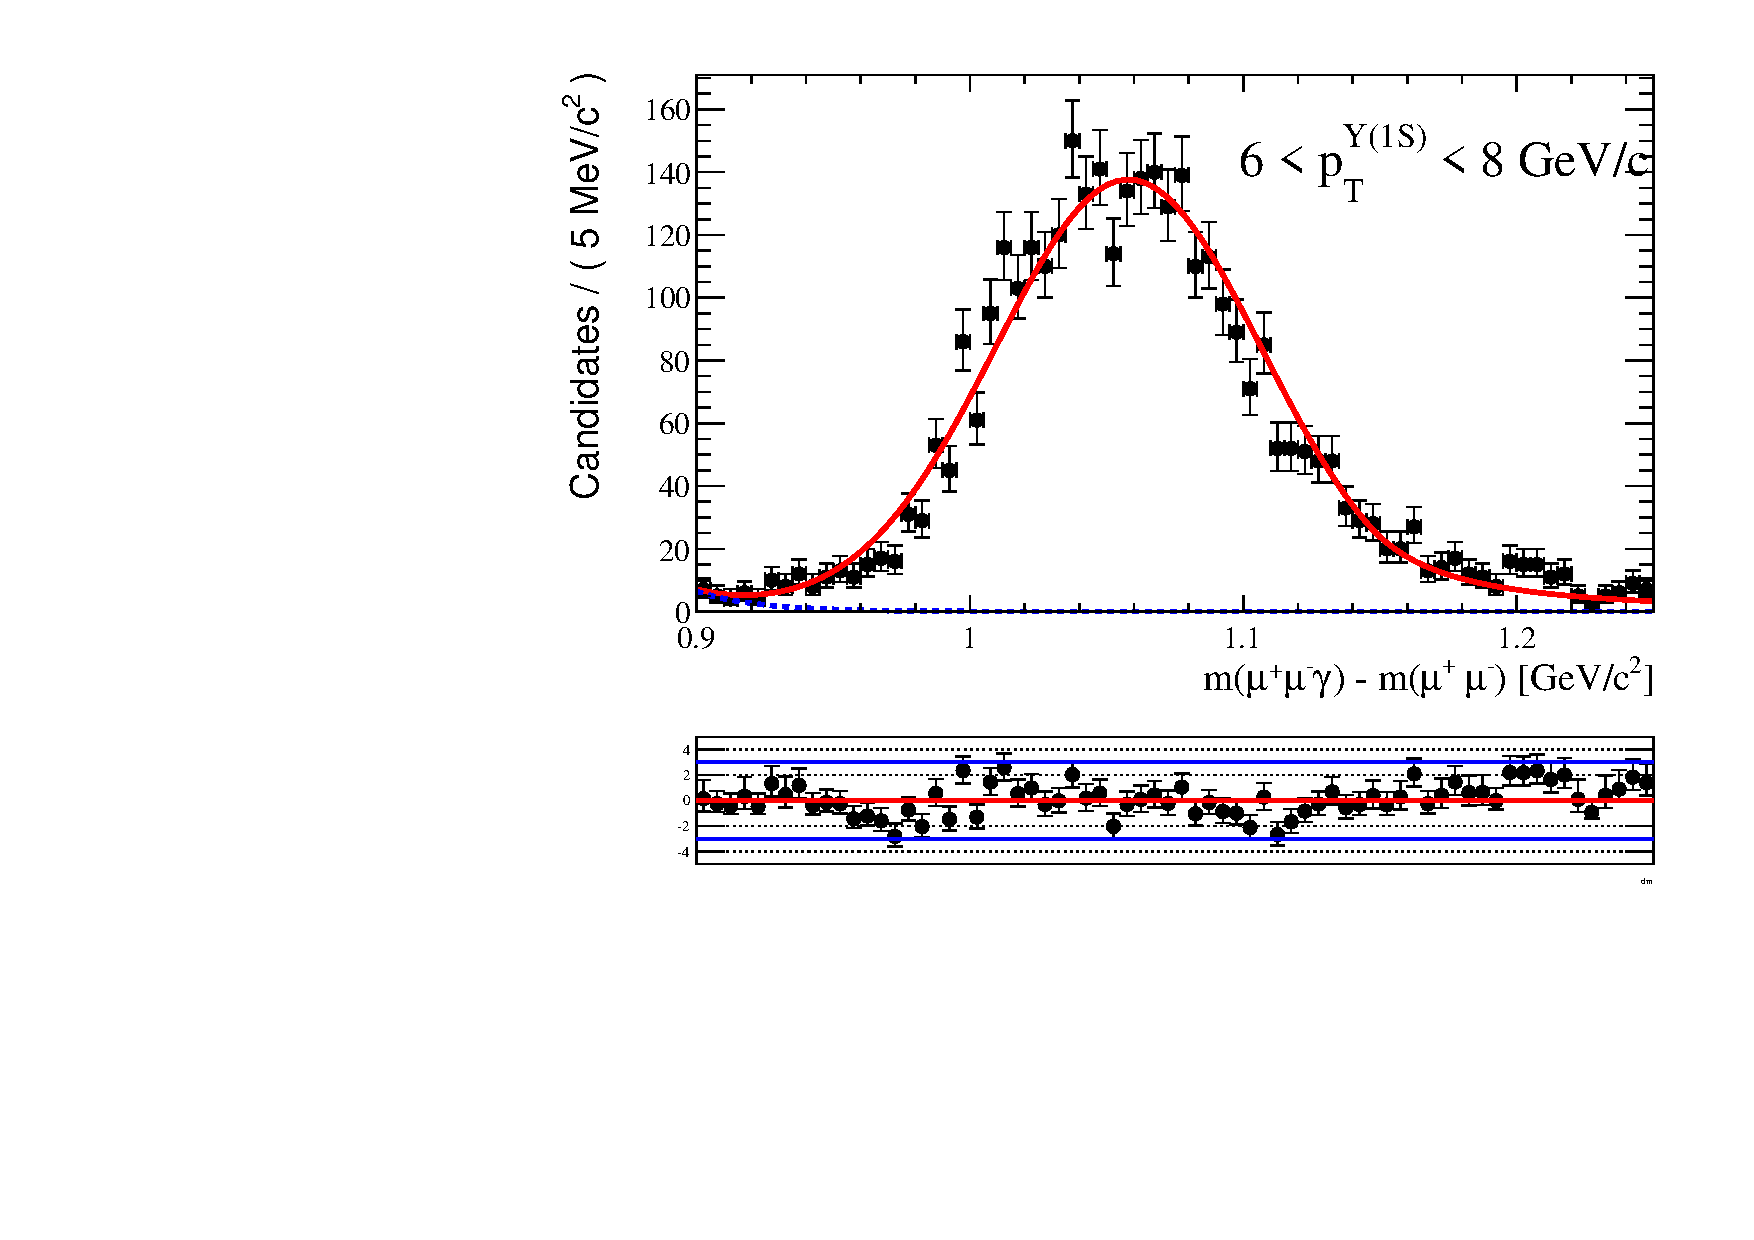
\includegraphics[width=0.16\linewidth]{fit_mc/chib23_6_8}
      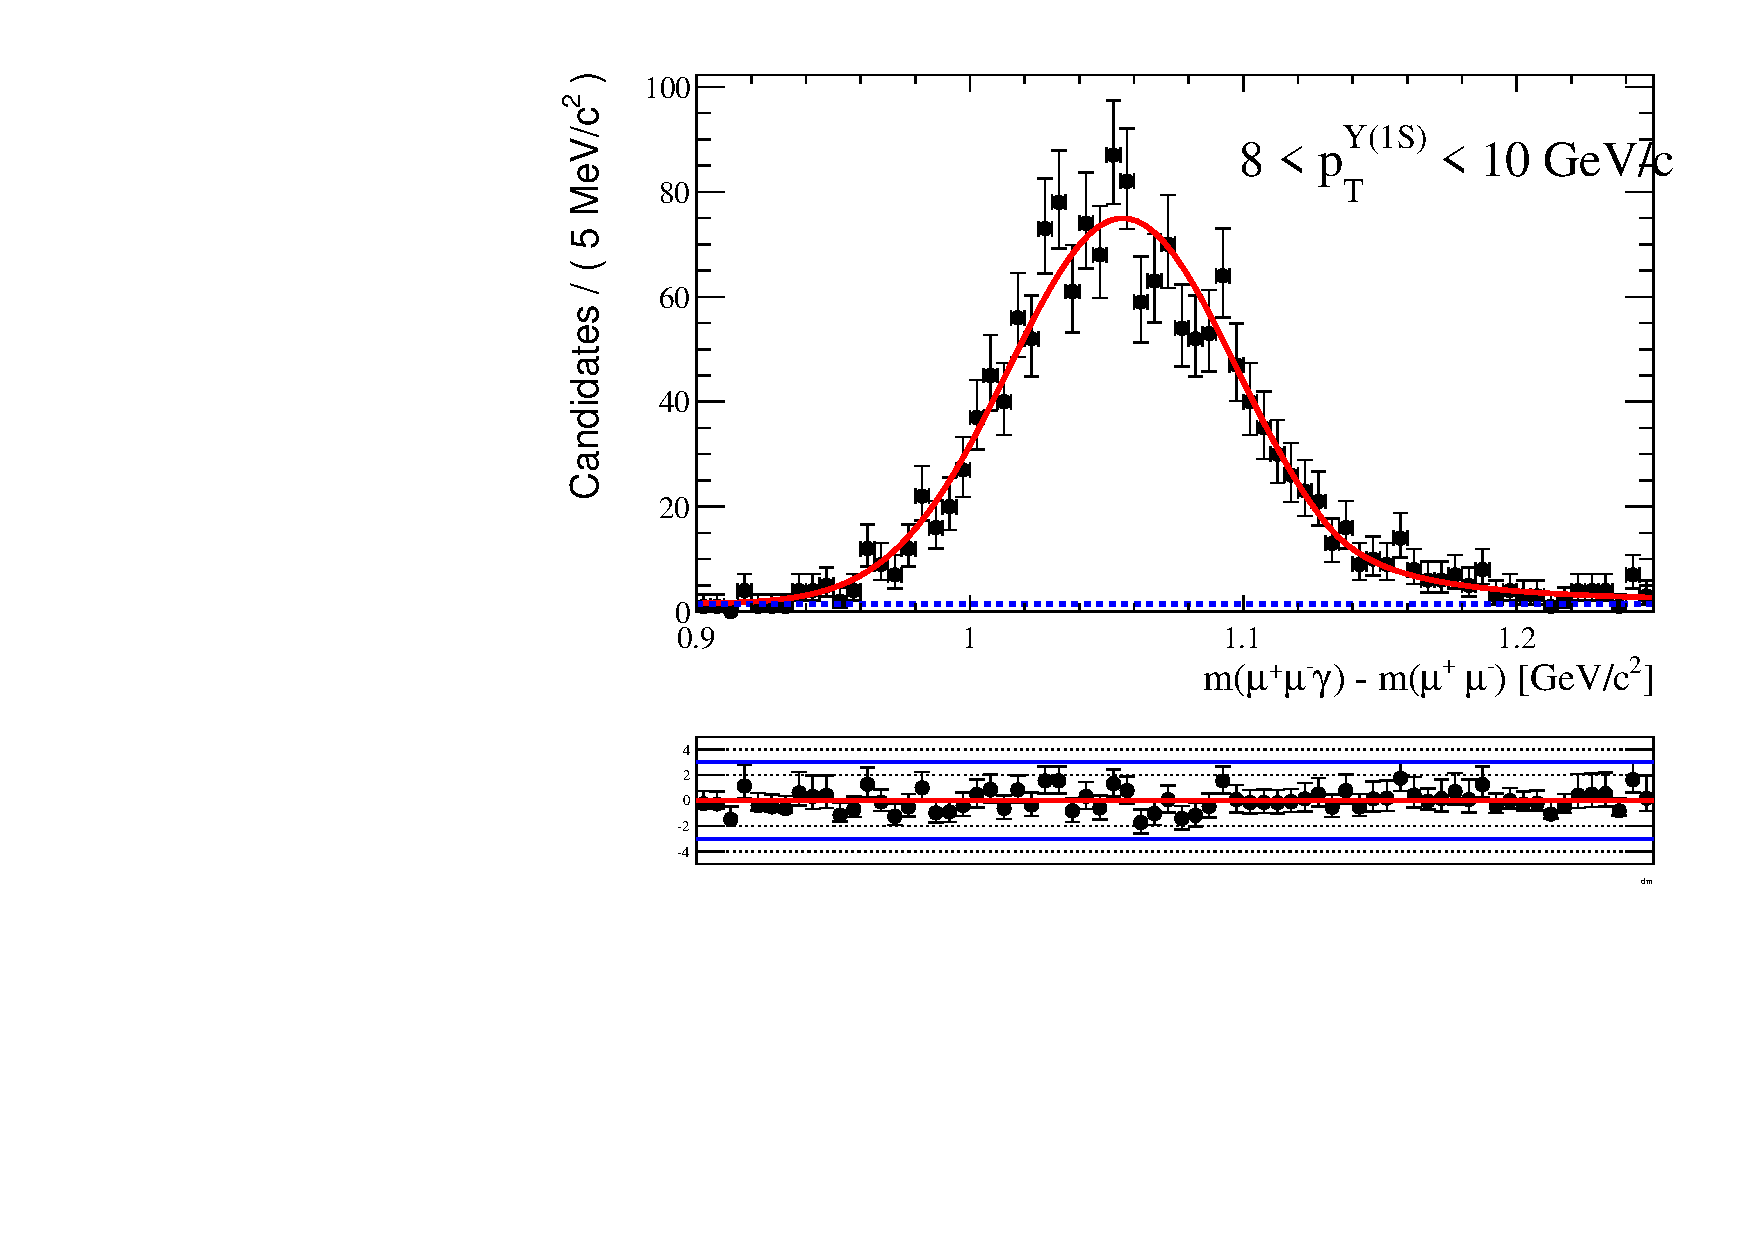
\includegraphics[width=0.16\linewidth]{fit_mc/chib23_8_10}
      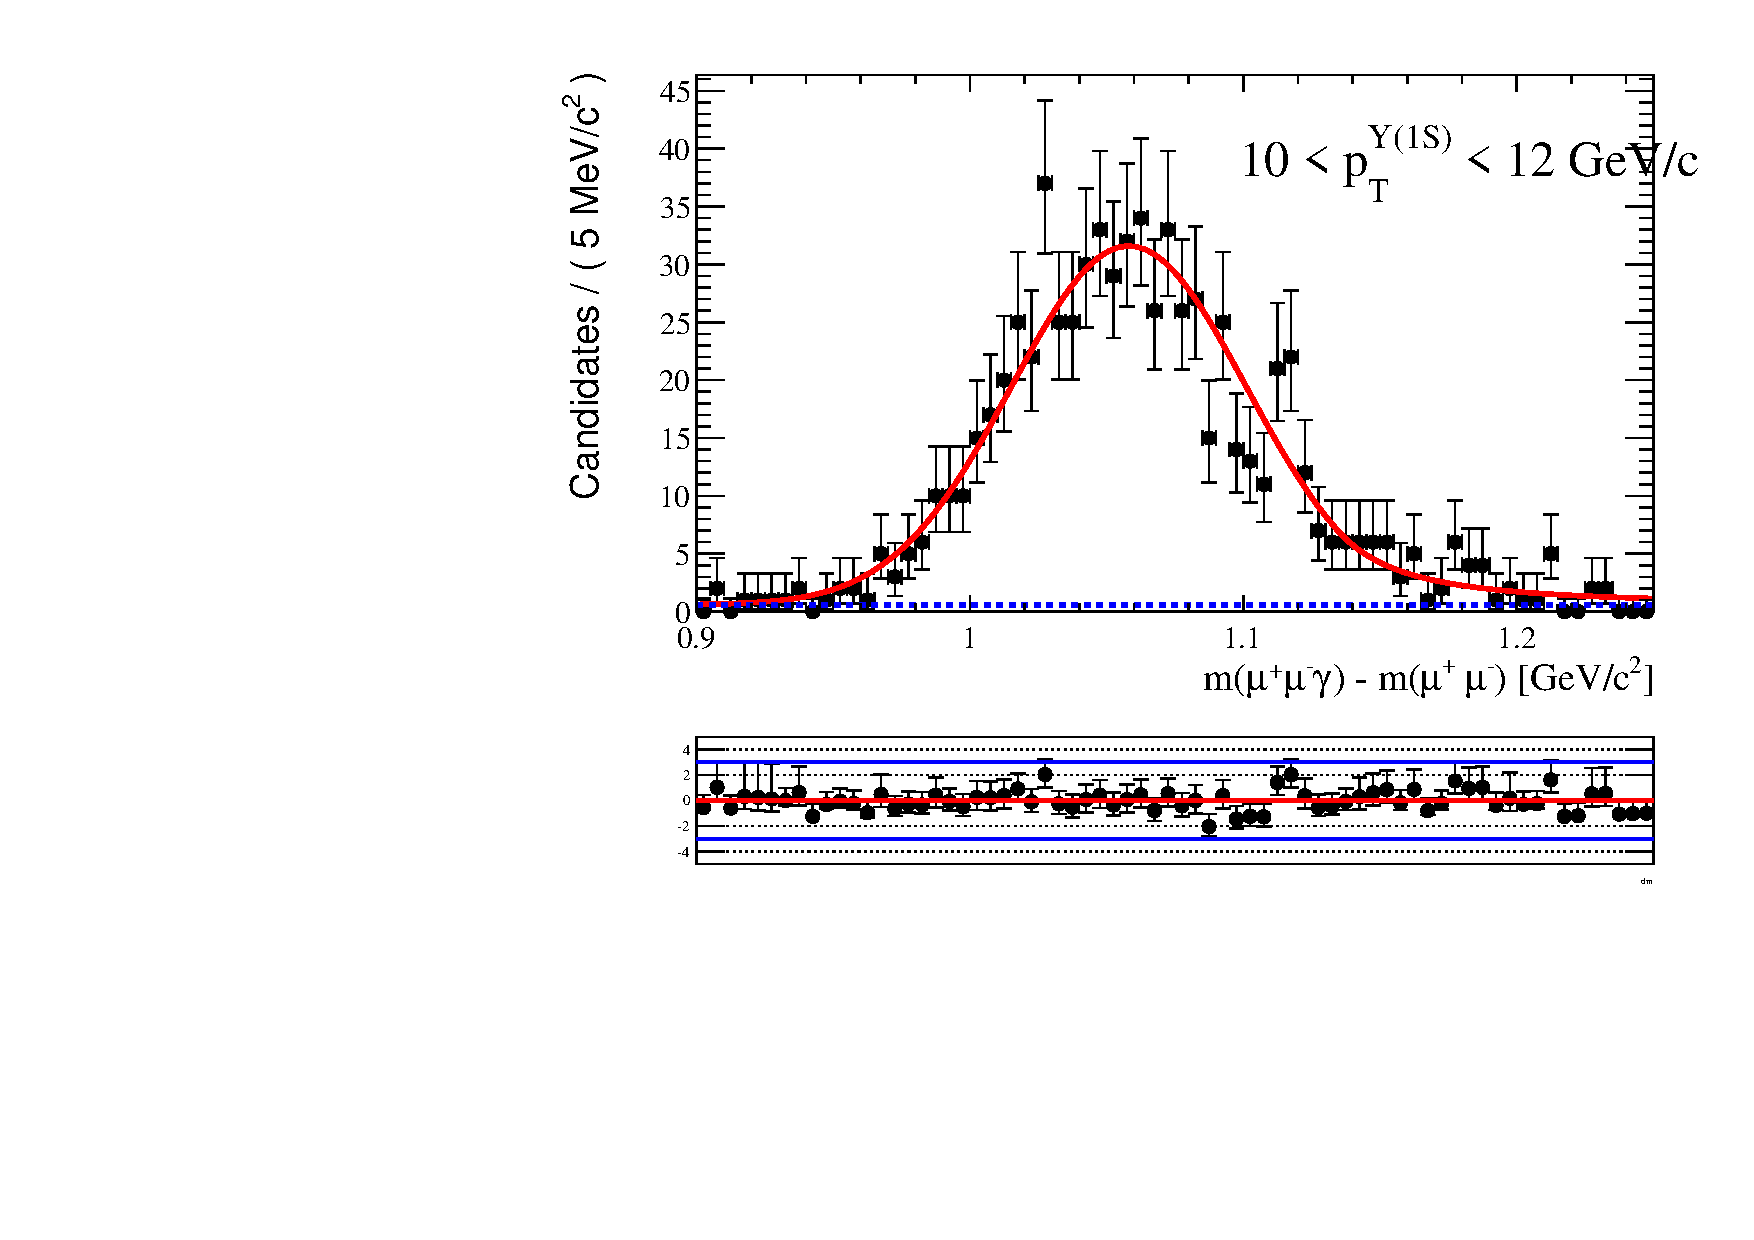
\includegraphics[width=0.16\linewidth]{fit_mc/chib23_10_12}
      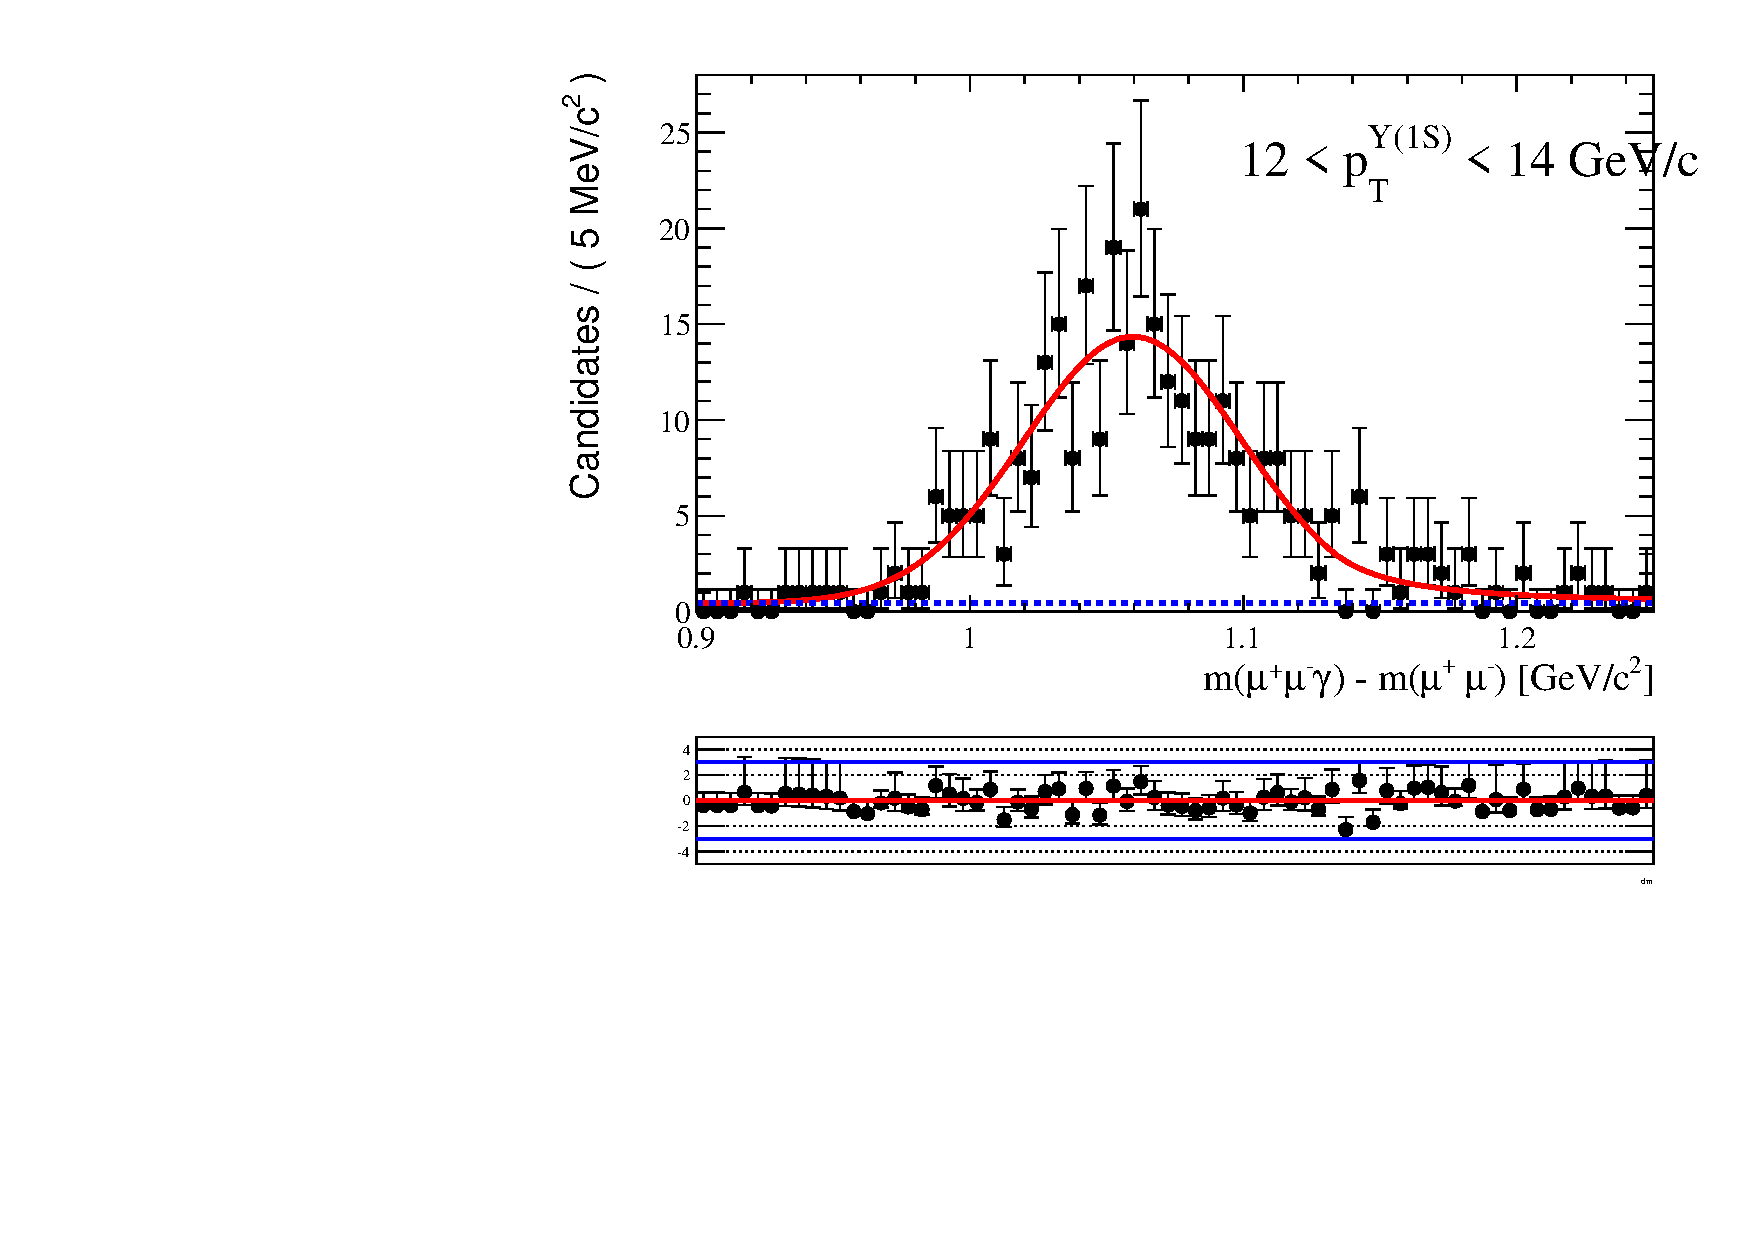
\includegraphics[width=0.16\linewidth]{fit_mc/chib23_12_14}
      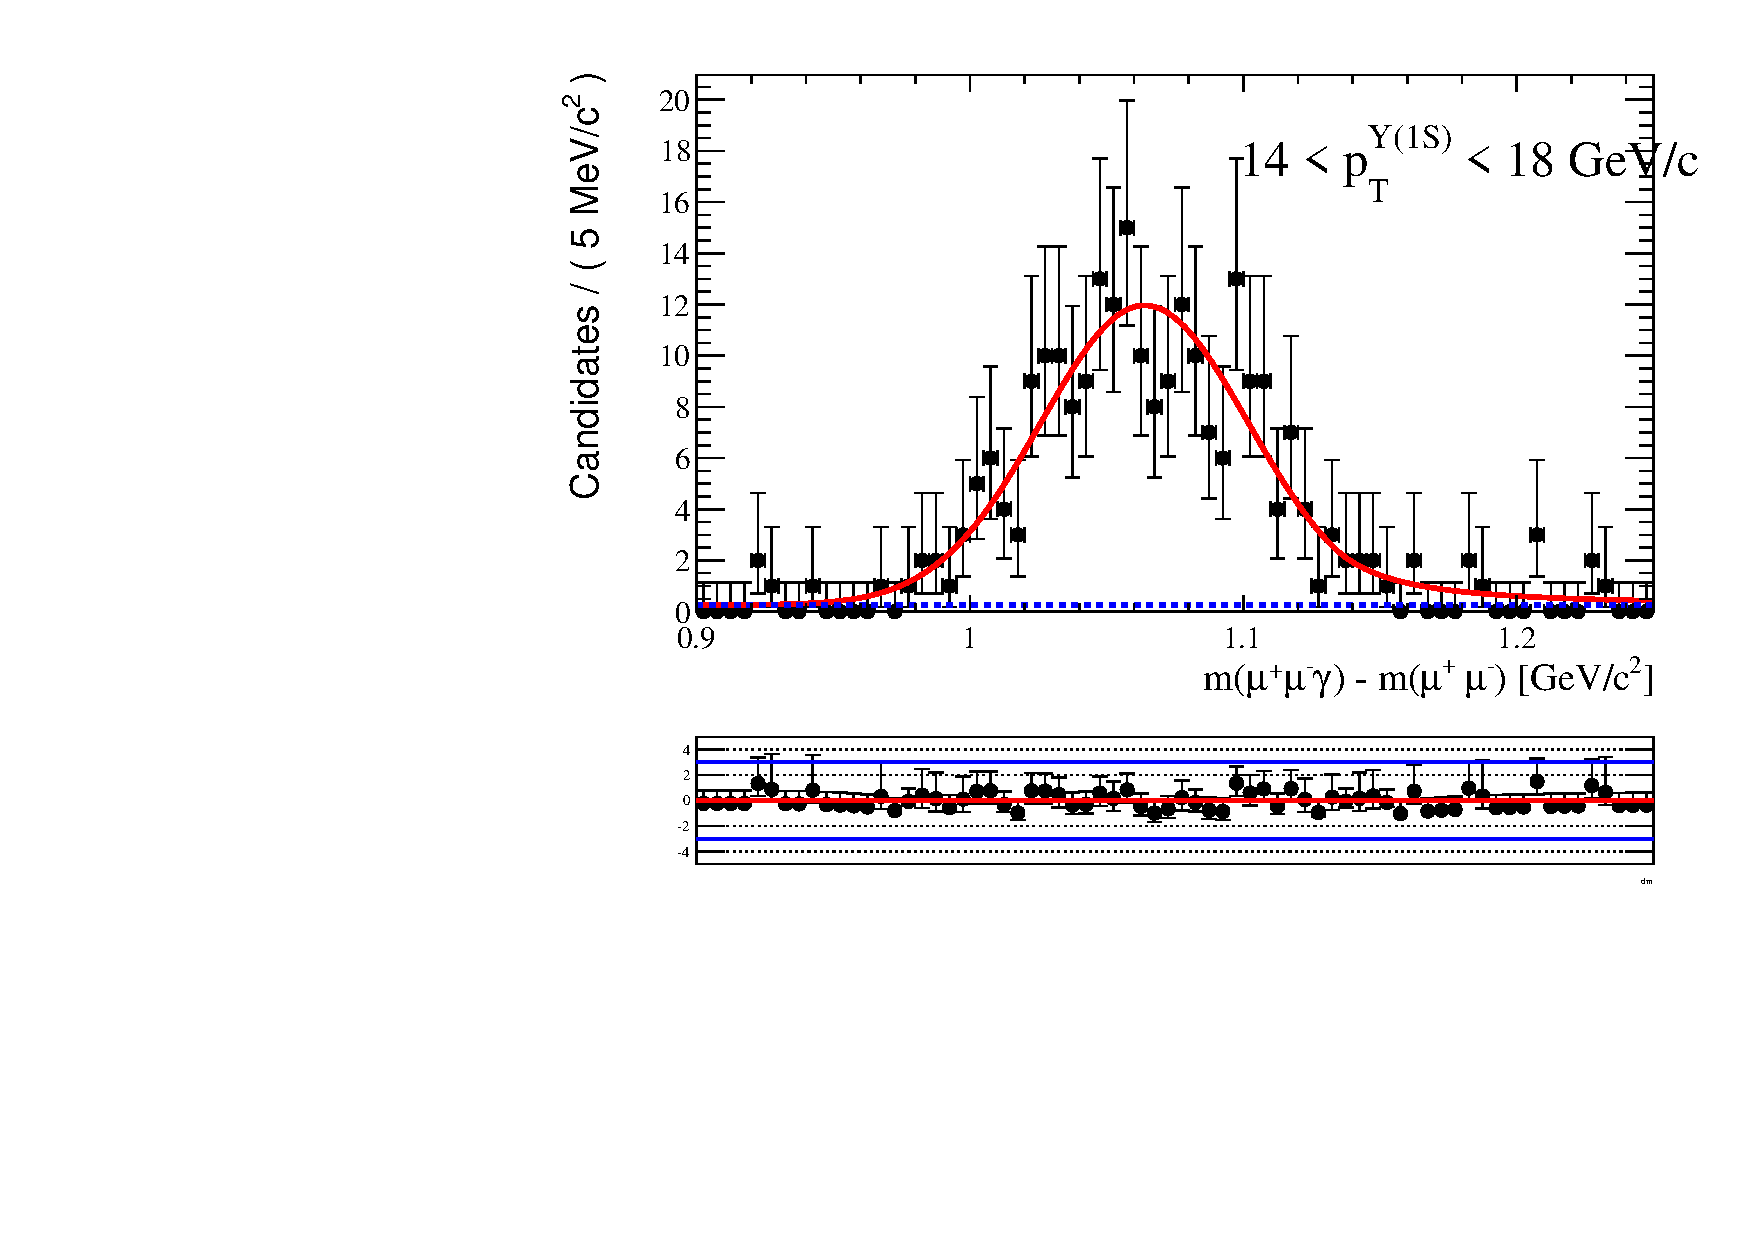
\includegraphics[width=0.16\linewidth]{fit_mc/chib23_14_18}
      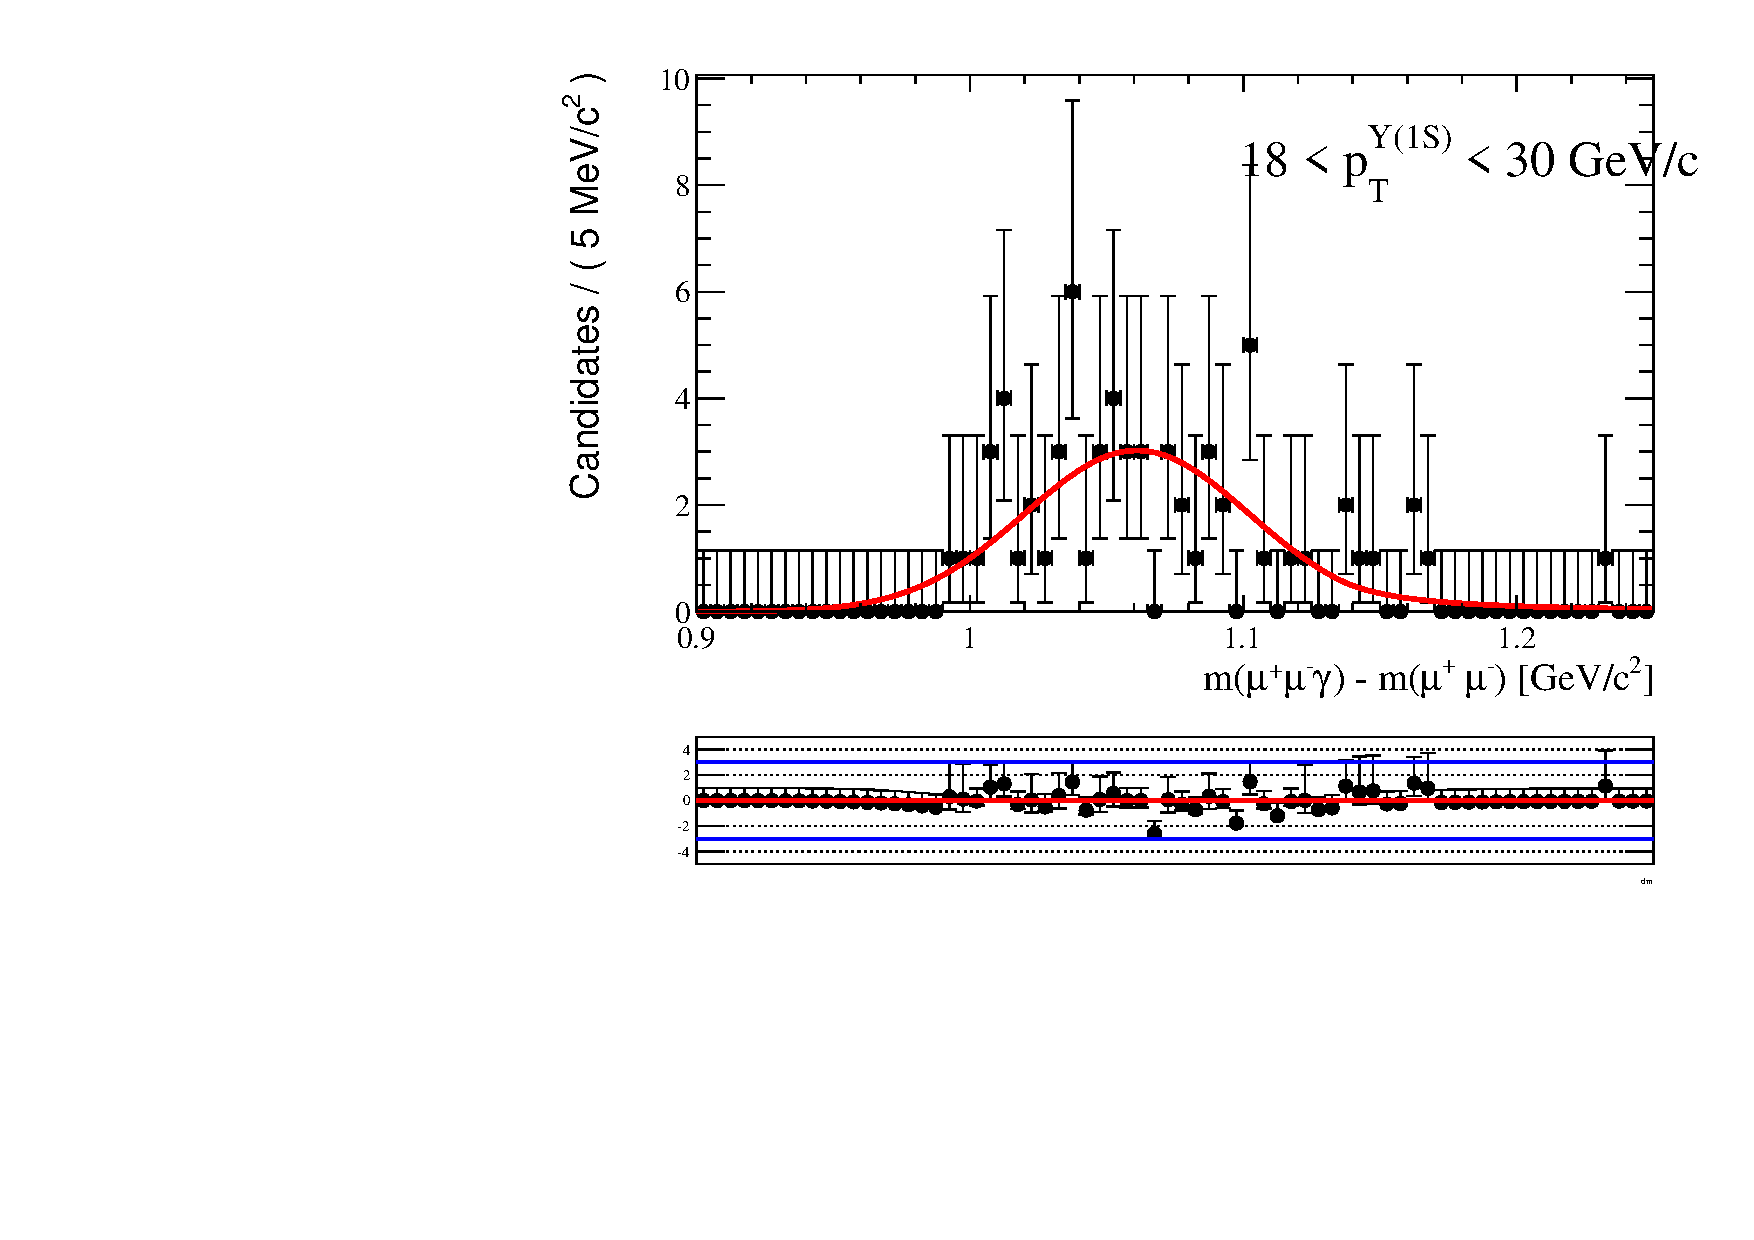
\includegraphics[width=0.16\linewidth]{fit_mc/chib23_18_30}
      \caption{\chibtwoThreeP}
      \label{fig:fit_mc_chibtwoThreeP}
    \end{subfigure}        
  \caption{
    \small  Mass difference of the $\mumu \gamma$ system and $\mumu$ system for the 
    Monte Carlo data for specified interval of transverse momentum of the \OneS. The red
    solid line is the result of the fit described in the text.
  }
  \label{fig:fit_mc}
\end{figure}

